% !TEX root =  main.tex


In this section, we demonstrate numerical results for computing the Casimir energy between two conducting objects, where the objects are spheres, Menger sponges,
ice crystals and ellipsoids. Reference values for the Casimir energy in each case is computed by grid refinement plus Richardson extrapolation.

%The reference value of the Casimir energy is computed by Richardson extrapolation method which is often used 
%for obtaining the higher-order estimate at zero grid spacing. Denote $\mathcal{E}_{\text{fine}}$ and $\mathcal{E}_{\text{coarse}}$ as the Casimir energy 
%numerically computed from the formula \eqref{KSSF and CasE} by setting the grid size $h$ as $h_{\text{fine}}$ and $h_{\text{coarse}}$ 
%($h_{\text{fine}}<h_{\text{coarse}}$), separately. Then, the high-accuracy result $\mathcal{E}_{\text{extrapolation}}$ can be generated from the following formula:
%\begin{align}\label{Richardson extrapolation}
%    \mathcal{E}_{\text{extrapolation}} \approx  \frac{h_{\text{coarse}}^{2}\mathcal{E}_{\text{fine}} - h_{\text{fine}}^{2}\mathcal{E}_{\text{coarse}}}{h_{\text{coarse}}^{2} - h_{\text{fine}}^{2}}.
%\end{align}

In the case of spheres we also compare with known asymptotic expansions \cite{emig2008casimir}.

\subsection{Two spheres case}
\begin{figure}[H]
    \hspace*{3cm}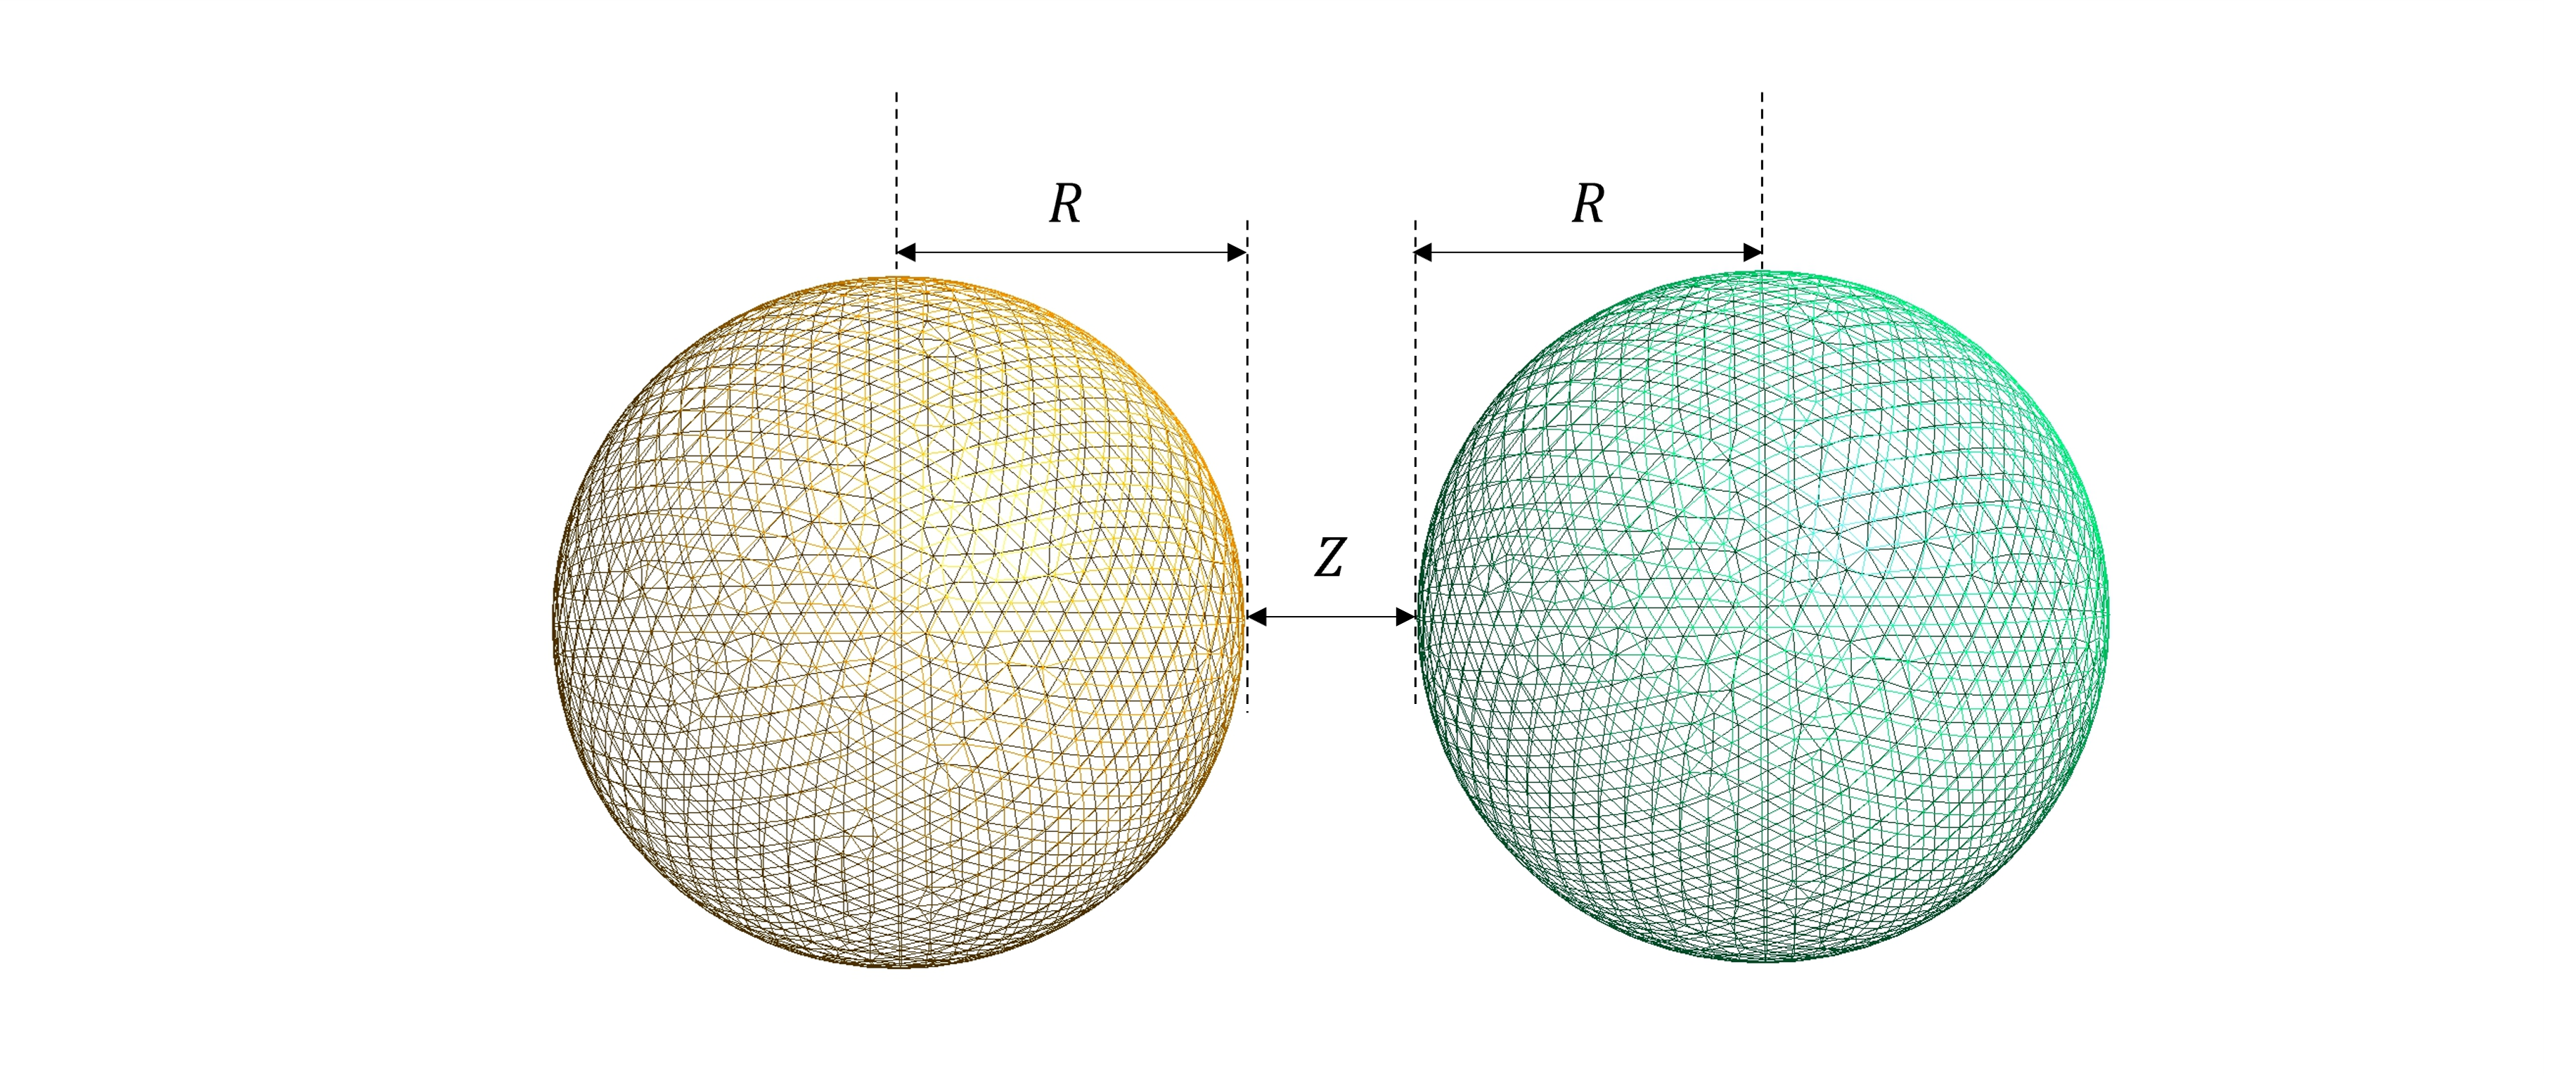
\includegraphics[scale = 0.6]{figures/Grid_two_spheres_dist.png}
    \caption{Two spheres with equal radii: $R = 1$ represents the radius of the spheres and $Z$ is the distance between them. 
    $h_{\text{coarse}} = 0.1$: $\text{dim}(\mathsf{V}_{\mathrm{i}k}) = 3192$,  N\textsuperscript{\underline{o}} of elements on both grids $ = 6384$;
    $h_{\text{fine}} = 0.05$: $\text{dim}(\mathsf{V}_{\mathrm{i}k}) = 12603$,  N\textsuperscript{\underline{o}} of elements on both grids $ = 25180$}
    \label{Two spheres with equal radii}
\end{figure}

Consider two perfectly conducting spheres with equal radii $R$ in Figure \ref{Two spheres with equal radii}. By denoting the distance between them as $Z$, 
the asymptotic expression of the integrand of the Casimir integral formula \eqref{KSSF and CasE} introduced in \cite{fang2021singularity} is written as:
\begin{align}\label{asymptotic integrand}
    \Xi(k) = -\frac{R_{1}R_{2}}{4Z(R_{1} + R_{2} + Z)}e^{2\mathrm{i}Zk} + o\left(e^{-2Z\text{Im}k}\right),
\end{align}
where $R_{1}$ and $R_{2}$ are the radius of the spheres.
{\color{red} I do not understand why you now use this expansion and in the earlier sentence cite \cite{emig2008casimir}. Is this the same expansion?}

{\color{red} As I have said when we discussed your thesis. It is terrible to start with this Figure. People want to see some kind of validation of your results.
But you compare with something that has quite different values.}

Figure \ref{Abs equal} plots the quotient of the leading term in \eqref{asymptotic integrand} and the estimated integrand value on different 
wavenumbers $\mathrm{i}k$. This quotient provides with a good estimate on the upperbound of the integration of the Casimir energy formula \eqref{KSSF and CasE}. 
For example, when the distance $Z = 1.5$, if $k$ in wavenumber $\mathrm{i}k$ is larger than 7, the quotient gets far away from 1, which means the approximated 
integrand value is not close to the asymptotic term and $7\mathrm{i}$ is chosen as the upperbound when $Z = 1.5$. The following table lists the upperbound 
of the integration for the distance $Z$ varying from 0.5 to 3.0.

\begin{table}[H]
    \centering
    \begin{tabular}{ |c|c|c|c|c|c|c|c|c|c|c|c| }
        \hline
        Distance $Z$ & $ 0.5$ & $ 0.75$  & $ 1.0$ & $1.25$ & $ 1.5$ & $1.75$  & $2.0$ & $2.25$ & $ 2.5$ & $ 2.75$  & $3.0$ \\\hline
        Upperbound & $24\mathrm{i}$ & $17\mathrm{i}$ & $13\mathrm{i}$ & $9\mathrm{i}$ & $7\mathrm{i}$ & $6\mathrm{i}$ & $6\mathrm{i}$ & $5\mathrm{i}$ & $5\mathrm{i}$ & $4\mathrm{i}$ & $4\mathrm{i}$ \\\hline
       \end{tabular}
       \caption{\label{Equal: distance and upperbound} The estimated upperbound for the Casimir energy formula for different minimal distance $Z$ varying from 
       0.5 to 3.0.}
\end{table}
 
\begin{figure}[H]
    \centering
    \hspace*{-1.4cm}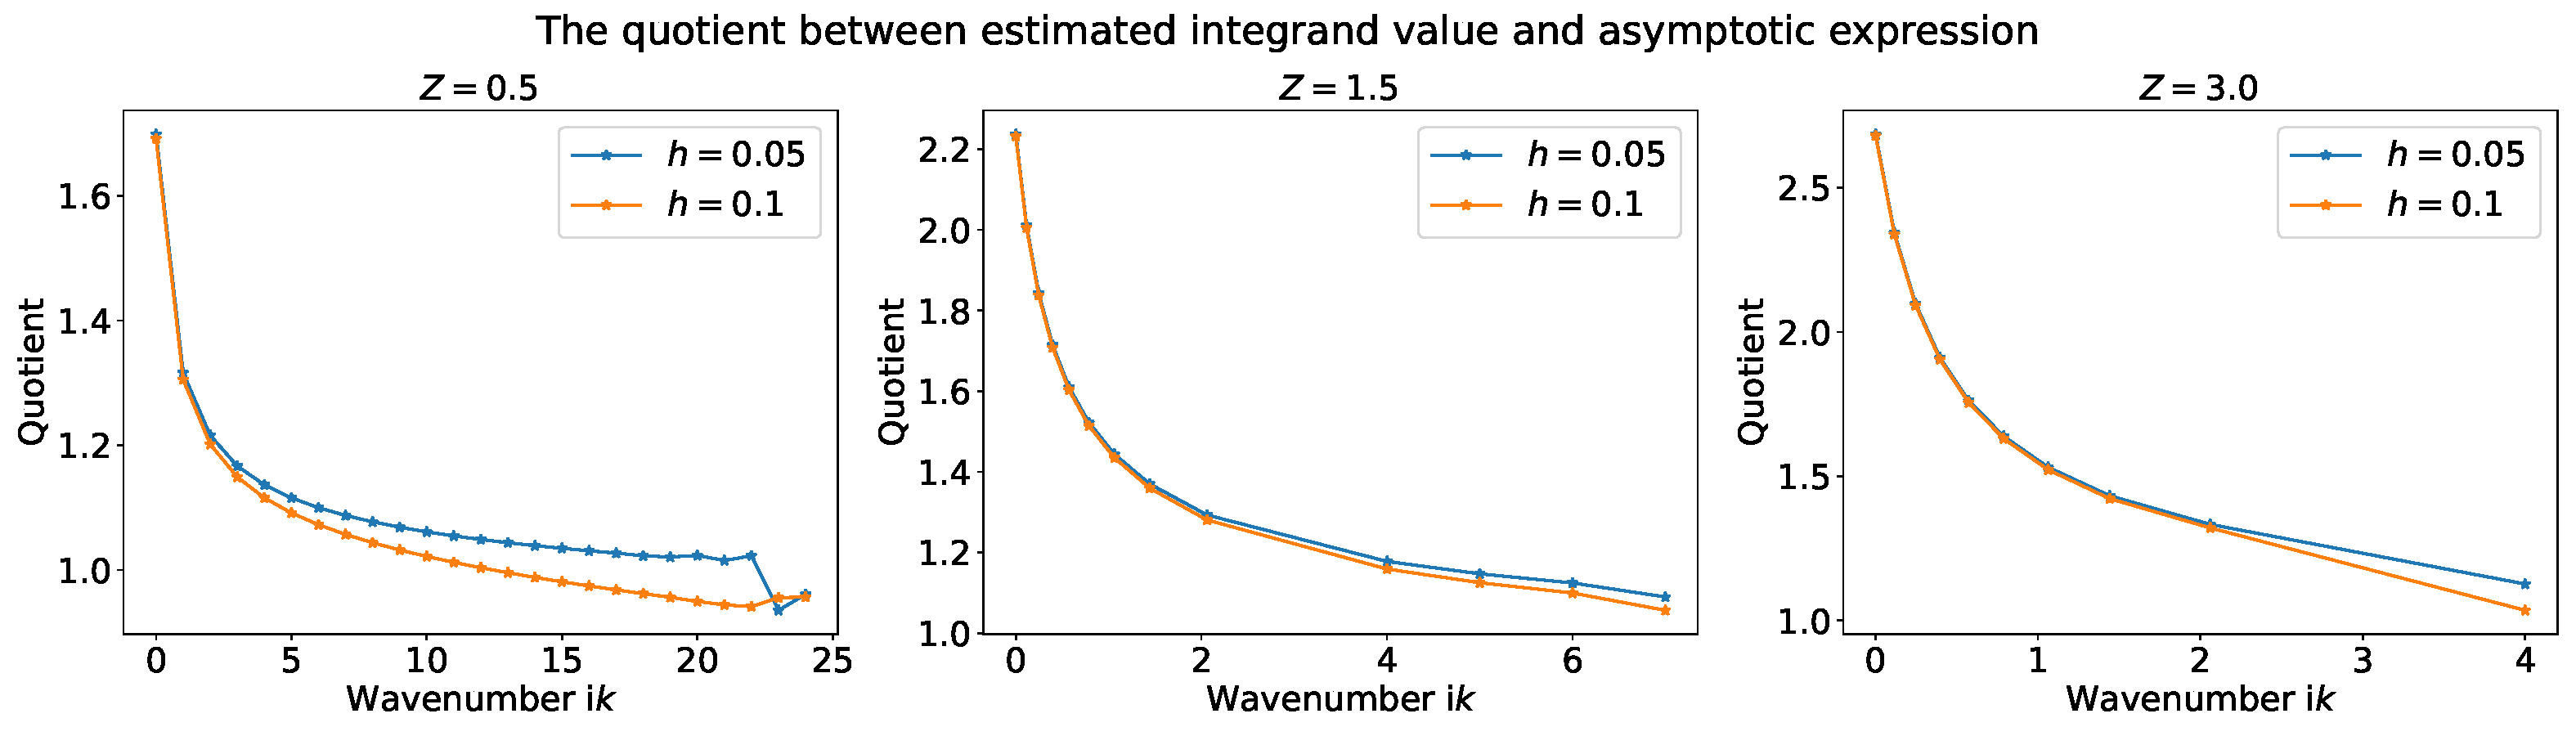
\includegraphics[scale = 0.37]{figures/rel_err_equal.pdf}
    \caption{The quotient of the leading term of the series \eqref{asymptotic integrand} and the estimated integrand value along the imaginary axis
    with grid size $h$ set as $h_{\text{coarse}} = 0.1$ and $ h_{\text{fine}} = 0.05$ in two spheres with equal radii's case. The radius of the spheres is $R = 1$ and the minimal distance between them is $Z = 0.5$, 1.5 and 3.0. }
    \label{Abs equal}
\end{figure}

\begin{remark}[Determine the upperbound of the integration from the error tolerance]\label{remark for upperbound determination}
    By Figure \ref{The integrand decays exponentially}, since the integrand value $\log\det\mathsf{V}_{\mathrm{i}k}\tilde{\mathsf{V}}_{\mathrm{i}k}^{-1}$ 
    shares the same trend with $e^{-2Zk}$ in \eqref{KSSF and CasE}, one can apply the function $f(k) = Ce^{-2Zk}$ to fit the curve of the estimated integrand
    values. With the coefficient $C$ determined, one can estimate the absolute error for approximating the Casimir integral by computing:  
    \begin{align*}
        \epsilon \approx \int_{\kappa}^{\infty}f(k)dk = \frac{Ce^{-2Z\kappa}}{2Z},
    \end{align*}
    where $\kappa$ is the upperbound of the integration. 
    
{\color{red} You earlier do a coordinate transformation. So this upper bound turns into a lower bound for your quadrature rule. You should remark on this}.
    
Meanwhile, one can also determine the upperbound of the integration with regard to different error tolerance. 

For example, if one aims to have at least three significant digits of the exact value of the Casimir integral, the upperbound can be set as the following 
table lists:

\begin{table}[H]
    \centering
    \begin{tabular}{ |c|c|c|c|c|c|c|c|c|c|c|c| }
        \hline
        Distance $Z$ & $ 0.5$ & $ 0.75$  & $ 1.0$ & $1.25$ & $ 1.5$ & $1.75$  & $2.0$ & $2.25$ & $ 2.5$ & $ 2.75$  & $3.0$ \\\hline
        Upperbound & $10\mathrm{i}$ & $7\mathrm{i}$ & $5\mathrm{i}$ & $5\mathrm{i}$ & $4\mathrm{i}$ & $3\mathrm{i}$ & $3\mathrm{i}$ & $2\mathrm{i}$ & $2\mathrm{i}$ & $2\mathrm{i}$ & $2\mathrm{i}$ \\\hline
       \end{tabular}
       \caption{\label{Equal: distance and upperbound error tolerance} The estimated upperbound for the Casimir energy formula for different minimal distance $Z$ varying from 
       0.5 to 3.0.}
\end{table}
\end{remark}

With the upperbound of the integration determined, one can start to estimate the Casimir energy between two spheres with radius $R = 1$ at the 
distance of $Z$ via the formula \eqref{KSSF and CasE} in two different refinement levels: $h_{\text{fine}} = 0.05$ 
($\text{dim}(\mathsf{V}_{\mathrm{i}k}) = 12603$) and $h_{\text{coarse}} = 0.1$ ($\text{dim}(\mathsf{V}_{\mathrm{i}k}) = 3192$).

Afterwards, the extrapolation result can be obtained by substituting these Casimir energy estimates into 
the formula \eqref{Richardson extrapolation}. This result would be regarded as the extrapolation value of the Casimir energy, which would be used to compare with the 
estimates derived from the asymptotic series introduced below. 

According to \cite{emig2008casimir}, the Casimir energy between two spheres (with equal radii $R$) at asymptotically 
large separations can be obtained as a series in terms of the ratio of centre distance $L$ ($L = 2R + Z$) to sphere radius $R$:
\begin{align}\label{Asymptotic equal radii}
   \mathcal{E} = -\frac{\hbar c}{\pi}\frac{1}{L}\sum_{n=0}^{\infty}b_{n}\left(\frac{R}{L}\right)^{n+2},
\end{align}
where the first six coefficients are 
$b_{0} = -1/4$, $b_{1} = -1/4$,  $b_{2} = -77/48$,  $b_{3} = -25/16$,  $b_{4} = -29837/2880$, $b_{5} = -6491/1152$. Figure 
\ref{Casimir energy between spheres with equal radii} shows the comparison between the Casimir energy computed from asymptotic series 
\eqref{Asymptotic equal radii} and the exact value evaluated through {Richardson extrapolation}. Here, we observe that the asymptotic value gradually 
approaches to the exact value as the distance $Z$ increases since the asymptotic expansion \eqref{Asymptotic equal radii} only works when the distance 
between two spheres is asymptotically large.

\begin{figure}[H]
    \centering
    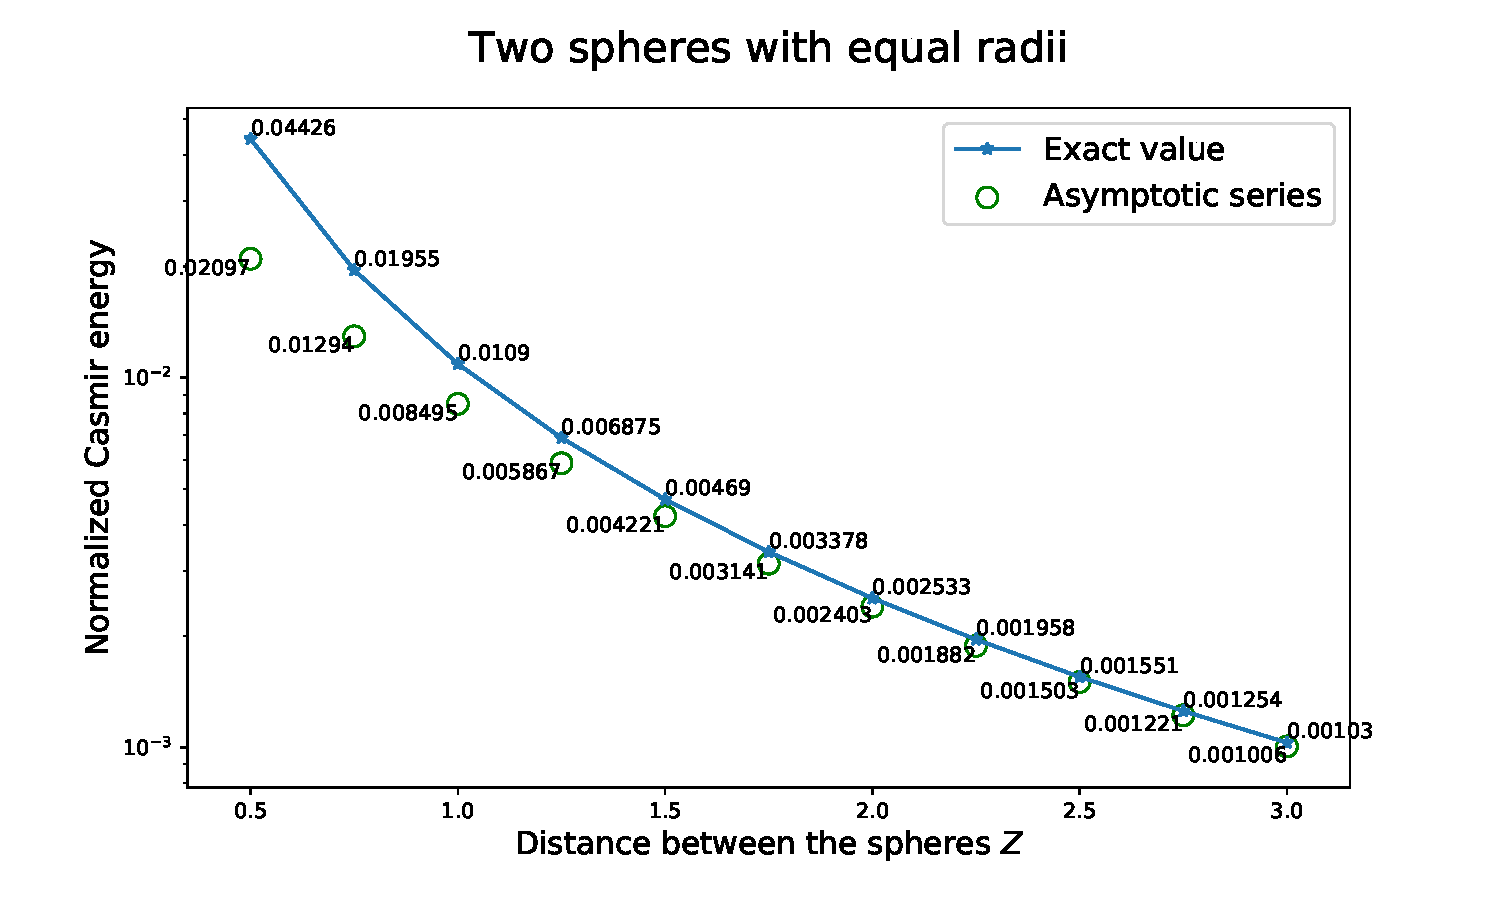
\includegraphics[scale = 0.5]{figures/Spheres_equal_CasE.pdf}
    \caption[Caption for LOF]{Normalized Casimir energy\protect\footnotemark in two spheres with equal radii's case. The radius is $R = 1$ and the distance $Z$ 
    ranges from 0.5 to 3.0. The exact value of the (normalized) Casimir energy has been written beside the data point, which is round up to 4 significant digits.}
    \label{Casimir energy between spheres with equal radii}
\end{figure}
\footnotetext{The normalized Casimir energy is $\mathcal{E}/\hbar c$, for $\mathcal{E}$ defined in \eqref{KSSF and CasE}.}

Figure \ref{equal_radii_rel_dist} shows the relative distance between the estimated Casimir energy computed through inverse-free Krylov subspace method with subspace 
recycled (solid blue triangles), standard Arnoldi method with subspace recycled (solid red circles), asymptotic series (solid black squares) and the extrapolation values.
For both efficient methods introduced in Section \ref{Krylov subspace for generalized eigenvalue problem}, the dimension of the Krylov subspace is set as $m = 100$. 
In addition, in the recycling process, only the eigenvectors associated with the extreme eigenvalues whose logarithm is larger than $10^{-5}$
would be extracted and recycled. With these settings, these two methods with subspace recycled can achieve at least three significant digits accuracy on 
approximating the Casimir energy.

\begin{figure}[H]
    \centering
    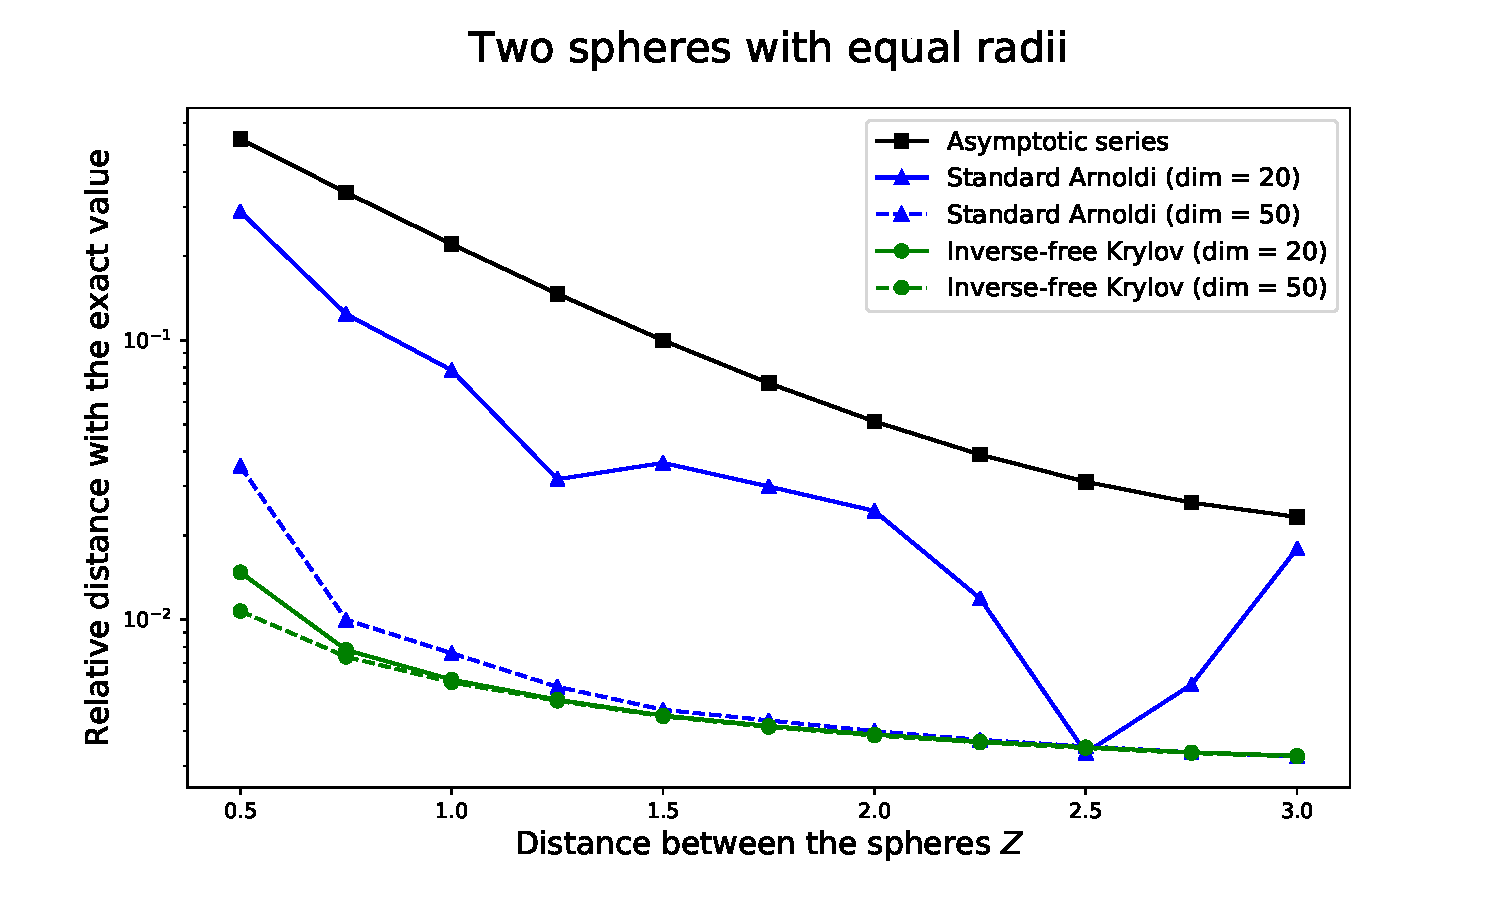
\includegraphics[scale = 0.5]{figures/relative_distance_equal_radii.pdf}
    \caption{Spheres with equal radii's case: relative distance between the reference value (computed by Richardson extrapolation) with the asymptotic series (solid black square)  
    and the estimates evaluated from the standard Arnoldi method with subspace recycled (solid red circles) and inverse-free Krylov subspace method 
    with subspace recycled (solid blue triangles). The dimension of the Krylov subspace is $m = 100$.}
    \label{equal_radii_rel_dist}
\end{figure}
 
%================================================================================================================
\begin{figure}[H]
    \hspace*{2cm}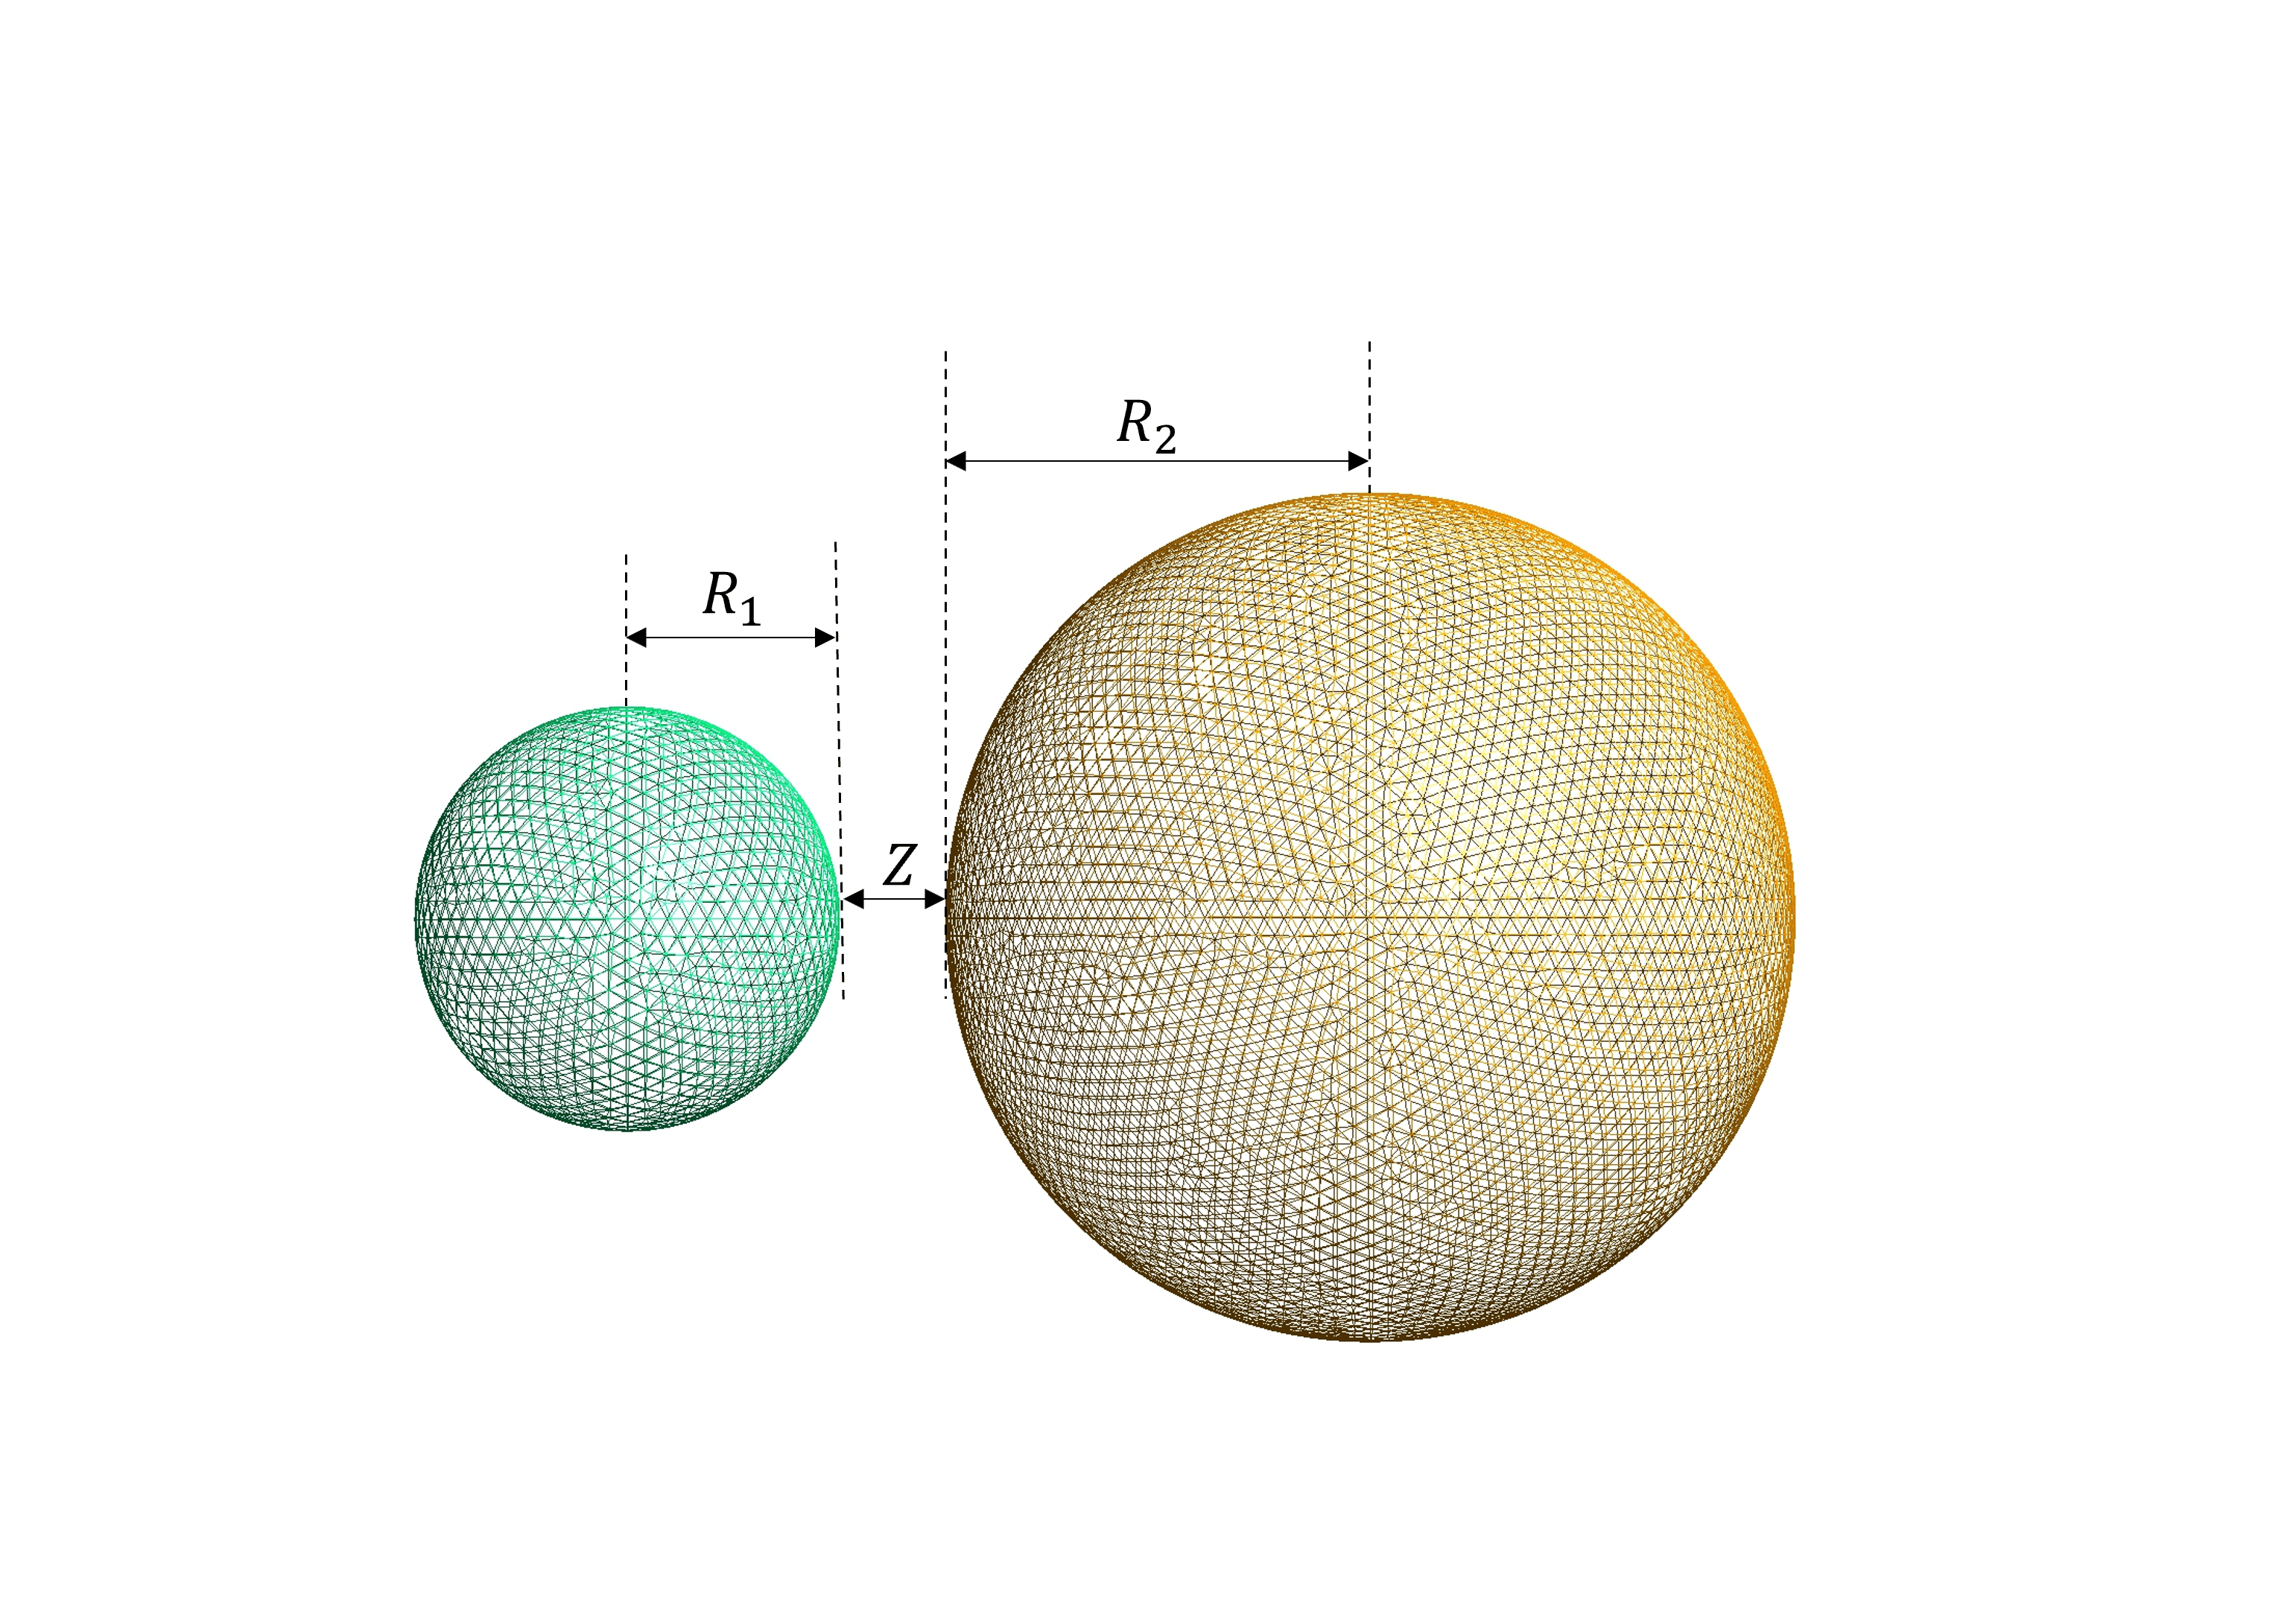
\includegraphics[scale = 0.6]{figures/Grid_two_spheres_unequal_radii.png}
    \caption{Two spheres with unequal radii: $R_{1} = 0.5$ and $R_{2} = 1$ represent the radius of the spheres and $Z$ is the distance between them.
    $h_{\text{coarse}} = 0.1$: $\text{dim}(\mathsf{V}_{\mathrm{i}k}) = 2023$,  N\textsuperscript{\underline{o}} of elements on both grids $ = 4038$;
    $h_{\text{fine}} = 0.05$: $\text{dim}(\mathsf{V}_{\mathrm{i}k}) = 7891$,  N\textsuperscript{\underline{o}} of elements on both grids $ = 15774$}
    \label{Two spheres with unequal radii}
\end{figure}

When the perfectly conducting spheres have different radii $R_{1}$, $R_{2}$ (see Figure \ref{Two spheres with unequal radii}), one can still use the 
asymptotic expansion \eqref{asymptotic integrand} to determine the upperbound of the integration in the Casimir energy formula. 

    \begin{figure}[H]
        \centering
        \hspace*{-1.4cm}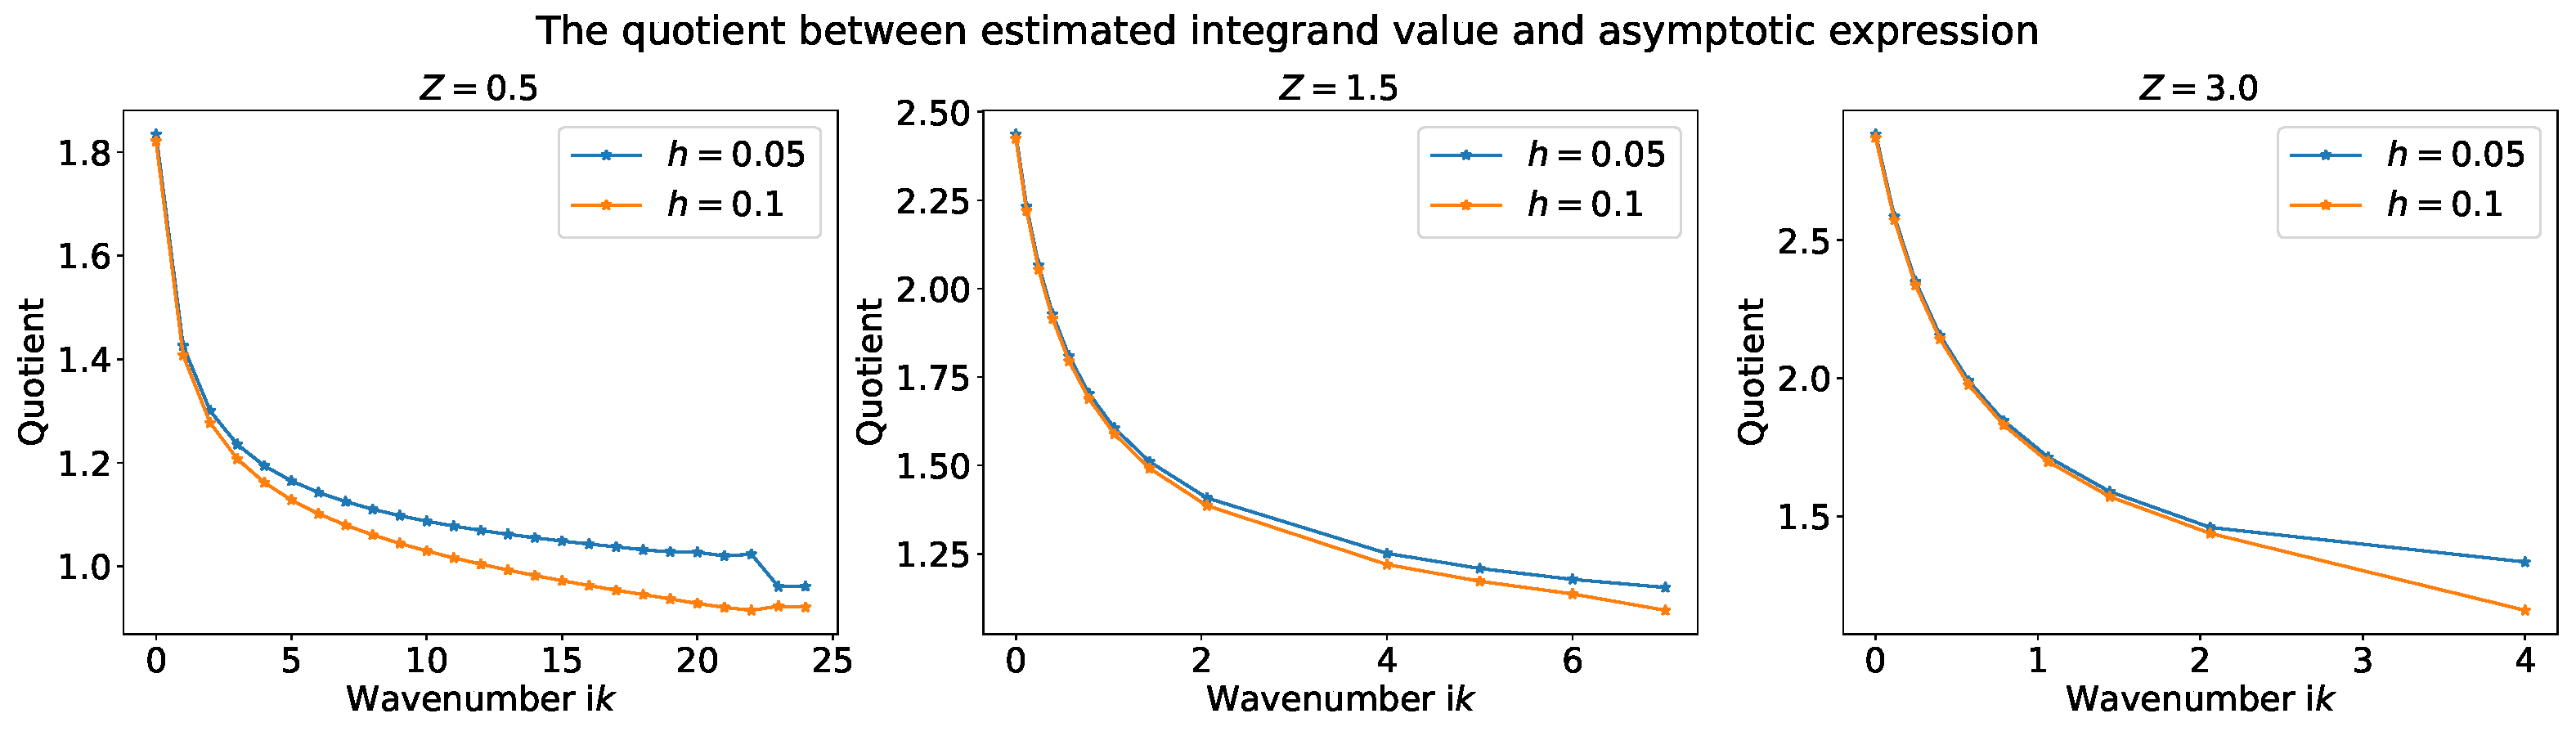
\includegraphics[scale = 0.37]{figures/rel_err_unequal.pdf}
        \caption{Absolute distance between the approximated integrand value of the Casimir energy formula and the first term in 
        asymptotic expansion \eqref{asymptotic integrand}, and compare this value with the exponential $e^{-2Z\text{Im}k}$. The radii of the spheres are equal to 
        $R_{1} = 1$ and $R_{2} = 0.5$, and the minimal distance $Z$ between them is 0.5, 1.5 and 3.0. The absolute distance is in solid blue triangles when grid size 
        $h = 0.1$ and in solid orange circles when $h = 0.05$.}
        \label{Abs unequal}
    \end{figure}

Again, with Figure \ref{Abs unequal}, one can easily estimate the upperbound and the results are listed in Table \ref{Unequal: distance and upperbound}.
\begin{table}[H]
    \centering
    \begin{tabular}{ |c|c|c|c|c|c|c|c|c|c|c|c| }
        \hline
        Distance $Z$ & $ 0.5$ & $ 0.75$  & $ 1.0$ & $1.25$ & $ 1.5$ & $1.75$  & $2.0$ & $2.25$ & $ 2.5$ & $ 2.75$  & $3.0$ \\\hline
        Upperbound & $24\mathrm{i}$ & $17\mathrm{i}$ & $13\mathrm{i}$ & $9\mathrm{i}$ & $7\mathrm{i}$ & $6\mathrm{i}$ & $6\mathrm{i}$ & $5\mathrm{i}$ & $5\mathrm{i}$ & $4\mathrm{i}$ & $4\mathrm{i}$ \\\hline
       \end{tabular}
       \caption{\label{Unequal: distance and upperbound} The estimated upperbound for the Casimir energy formula for different minimal distance $Z$ varying from 
       0.5 to 3.0.}
\end{table}

By recalling the Remark \ref{remark for upperbound determination}, in order to have at least three significant digits matching with the exact value of the Casimir
energy, the upperbound can be set as:
\begin{table}[H]
    \centering
    \begin{tabular}{ |c|c|c|c|c|c|c|c|c|c|c|c| }
        \hline
        Distance $Z$ & $ 0.5$ & $ 0.75$  & $ 1.0$ & $1.25$ & $ 1.5$ & $1.75$  & $2.0$ & $2.25$ & $ 2.5$ & $ 2.75$  & $3.0$ \\\hline
        Upperbound & $10\mathrm{i}$ & $6\mathrm{i}$ & $6\mathrm{i}$ & $4\mathrm{i}$ & $4\mathrm{i}$ & $3\mathrm{i}$ & $3\mathrm{i}$ & $3\mathrm{i}$ & $3\mathrm{i}$ & $3\mathrm{i}$ & $3\mathrm{i}$ \\\hline
       \end{tabular}
       \caption{\label{Unqual: distance and upperbound error tolerance} The estimated upperbound for the Casimir energy formula for different minimal distance $Z$ varying from 
       0.5 to 3.0.}
\end{table}


Afterwards, by denoting the centre distance as
$L = R_{1} + R_{2} + Z$, the asymptotic expansion of the Casimir energy at asymptotically large distance can be written as:
\begin{align}\label{Asymptotic unequal radii}
    \mathcal{E} = -\frac{\hbar c}{\pi}\frac{1}{L}\sum_{n=0}^{\infty}\tilde{b}_{n}(\eta)\left(\frac{R_{1}}{L}\right)^{n+2},
\end{align}
where the coefficients $\{\tilde{b}_{n}\}$ depend on the parameter $\eta = R_{2}/R_{1}$ and the first six coefficients are
\begin{align*}
    \tilde{b}_{0} &= -\frac{\eta}{4}, \ \ \ \ \ \tilde{b}_{1} = -\frac{\eta + \eta^{2}}{8}, \ \ \ \ \  \tilde{b}_{2} = -\frac{34(\eta+\eta^{3})+ 9\eta^{2}}{48}, \ \ \ \ \ \tilde{b}_{3} = -\frac{2(\eta+\eta^{4}) + 23(\eta^{2} + \eta^{3})}{32}, \\ 
    \tilde{b}_{4} &= -\frac{8352(\eta + \eta^{5})+ 1995(\eta^{2} + \eta^{4}) + 38980\eta^{3}}{5760}, \ \ \ \ \ \tilde{b}_{5} = -\frac{-1344(\eta+\eta^{6}) + 5478(\eta^{2} + \eta^{5})+2357(\eta^{3} + \eta^{4})}{2304}.
\end{align*}

In the following experiment, the radii of the spheres shown in Figure \ref{Two spheres with unequal radii} are set as $R_{1} = 0.5$ and $ R_{2} = 1$. 
As in the previous example, the exact value of the Casimir energy is computed through the Richardson extrapolation formula \eqref{Richardson extrapolation}, 
where the coarse and fine grid size are $h_{\text{fine}} = 0.05$ ($\text{dim}(\mathsf{V}_{\mathrm{i}k}) = 7893)$ and 
$h_{\text{coarse}} = 0.1$ ($\text{dim}(\mathsf{V}_{\mathrm{i}k}) = 2023)$, separately. 


In this case, the asymptotic value of the Casimir 
energy was estimated by the series \eqref{Asymptotic unequal radii} and the comparison between the exact value and asymptotic one is shown in Figure 
\ref{Casimir energy between spheres with unequal radii}. Again, one can notice that when the distance between two spheres decreases, the asymptotic value gets 
close to the exact one and the reason for this is clearly stated in the above equal radii's case.
\begin{figure}[H]
    \centering
    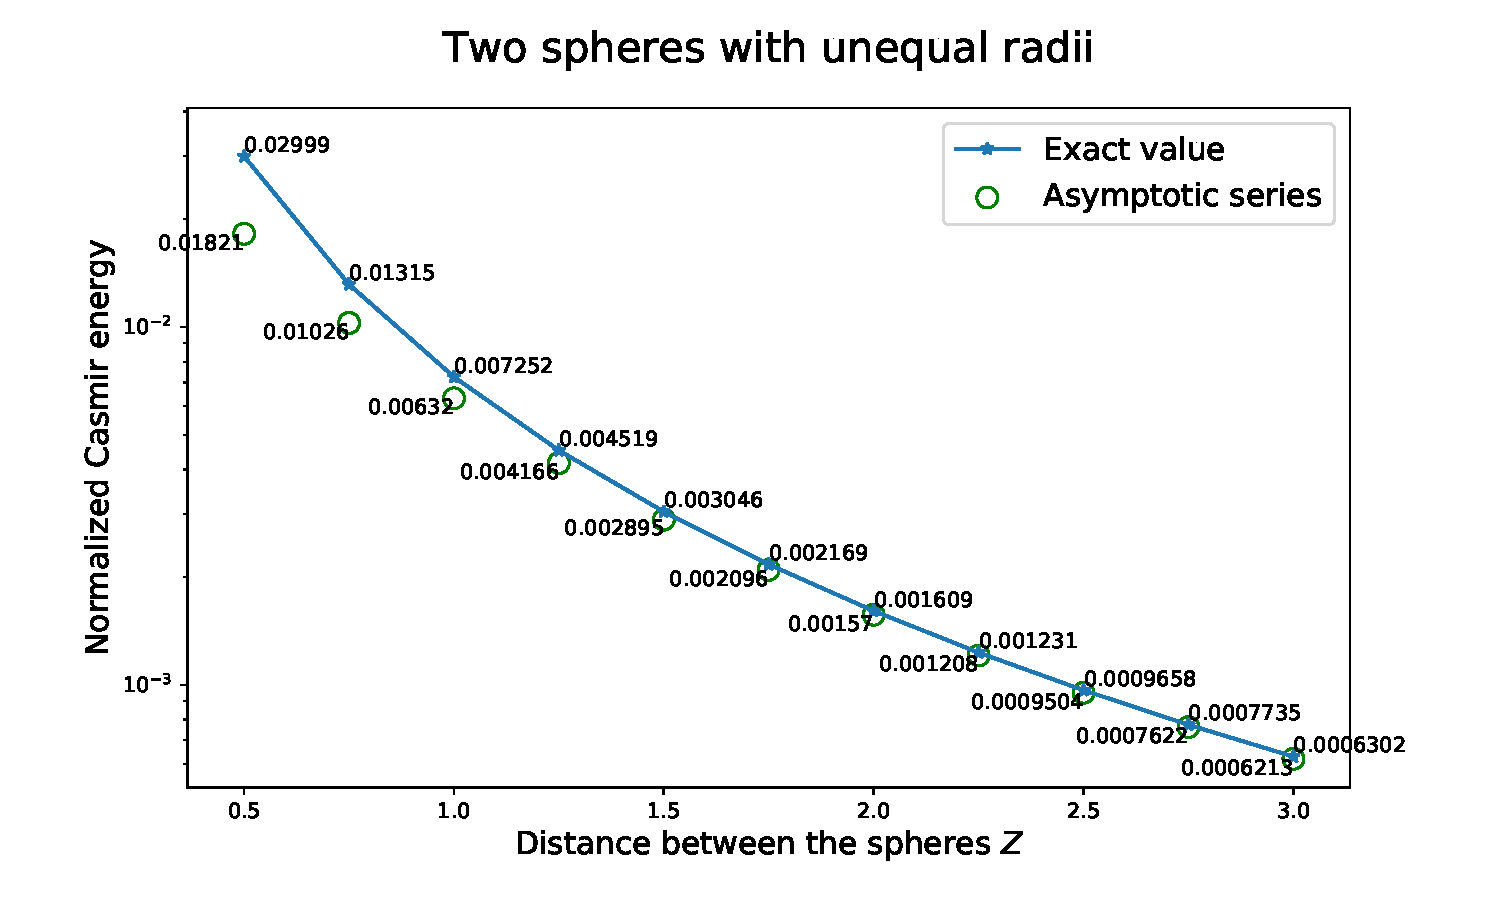
\includegraphics[scale = 0.5]{figures/Spheres_unequal_CasE.pdf}
    \caption{Normalized Casimir energy in two spheres with unequal radii's case. The radius is $R = 1$ and the distance $Z$ 
    ranges from 0.5 to 3.0. The exact value of the (normalized) Casimir energy has been written 
    beside the data point, which is round up to 4 significant digits.}
    \label{Casimir energy between spheres with unequal radii}
\end{figure}

By keeping all the experimental settings being the same with the equal radii's case, the numerical experiments on testing the performance of the inverse-free and 
standard Arnoldi methods with subspace recycled have been done in the unequal radii's case and the results are shown in Figure \ref{unequal_radii_rel_dist}.

\begin{figure}[H]
    \centering
    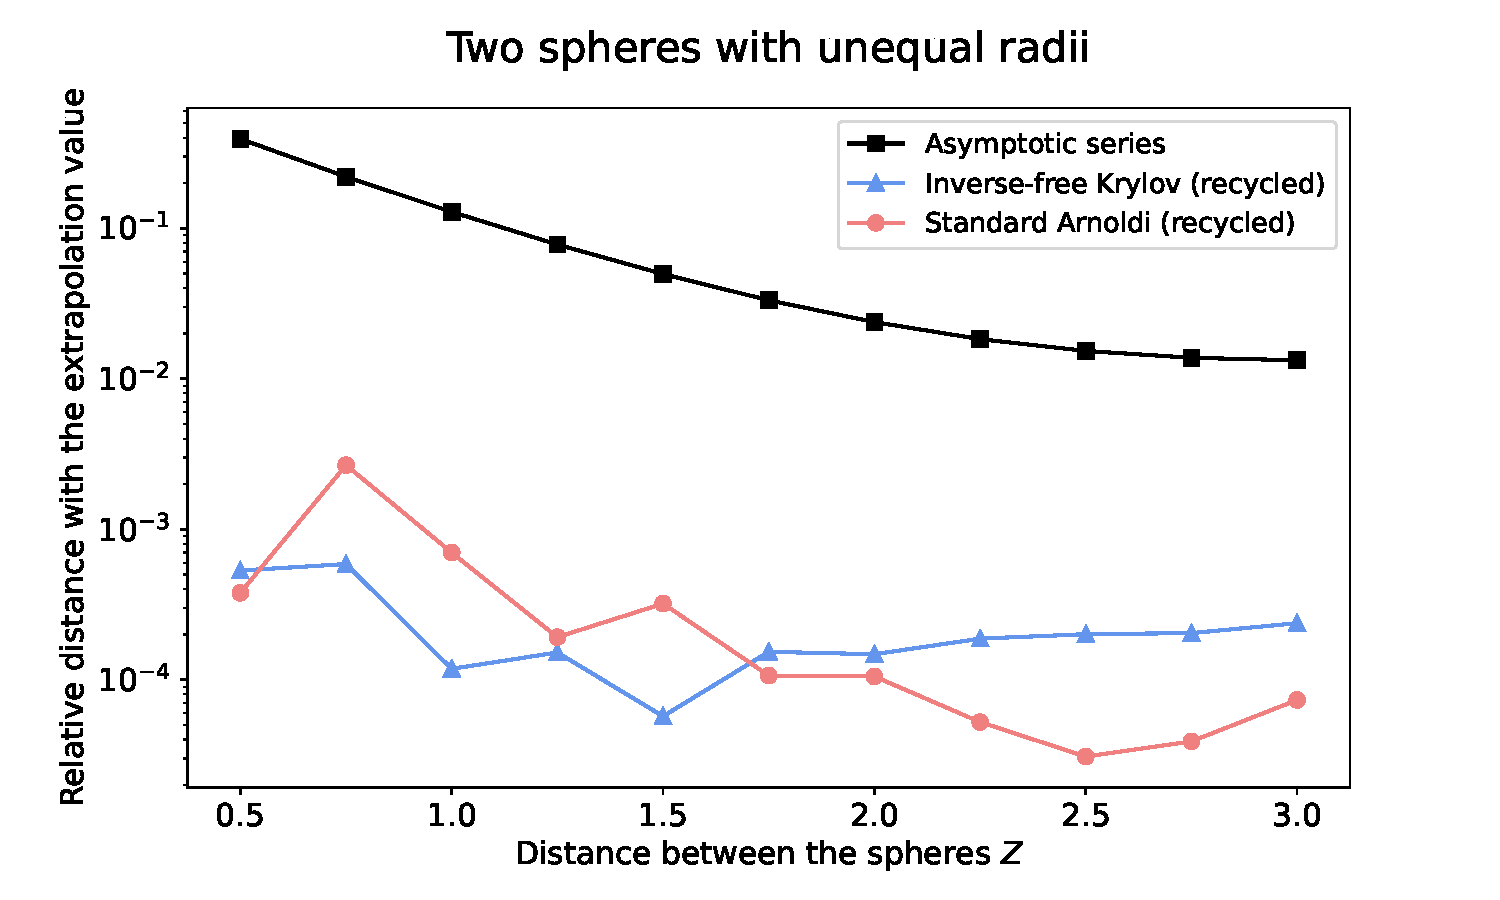
\includegraphics[scale = 0.5]{figures/relative_distance_unequal_radii.pdf}
    \caption{Spheres with unequal radii's case: relative distance between the reference value (computed by Richardson extrapolation) with the asymptotic series (solid black square)  
    and the estimates evaluated from the standard Arnoldi method with subspace recycled (solid red circles) and inverse-free Krylov subspace method 
    with subspace recycled (solid blue triangles). The dimension of the Krylov subspace is $m = 100$.}
    \label{unequal_radii_rel_dist}
\end{figure}

\subsection{Realistic objects case}
In this part, the Casimir energy between the objects with special shapes such as the menger sponges, ice crystals and ellipsoids will be computed 
through the Richardson extrapolation mentioned in the beginning of this section and the values labelled in the following figures are always round up to 4 significant digits. 

Figure \ref{Menger sponges} plots the menger sponges in different levels $(0, 1 $ and $ 2)$ and the length of these sponges is always 1. Afterwards, the Casimir 
energy between two menger sponges in the same level are listed in Table \ref{Normalized Casimir energy in two menger sponges' case}. 
In addition, inside the extrapolation process, when $h_{\text{fine}} = 0.05$, the $\text{dim}(\mathsf{V}_{\mathrm{i}k}) = 5664$, 8510 and 27136 and 
when $h_{\text{coarse}} = 0.1$, the $\text{dim}(\mathsf{V}_{\mathrm{i}k}) = 1456$, 3092 and 14464 in different level (0, 1 and 2) cases, separately. 
By comparing the data 
point in this table, it is easy to find that the Casimir energy decreases as the number of the iteration increases since the cross-sectional 
area gets smaller.

\begin{figure}[H]
    \centering
    \captionsetup[subfigure]{justification=centering}
    \subfloat[Level 0 \\ $h_{\text{coarse}} = 0.1$: $\text{dim}(\mathsf{V}_{\mathrm{i}k}) = 1456$,  N\textsuperscript{\underline{o}} of elements on both grids $ = 2904$
    \\ $h_{\text{fine}} = 0.05$: $\text{dim}(\mathsf{V}_{\mathrm{i}k}) = 5664$,  N\textsuperscript{\underline{o}} of elements on both grids $ = 11120$]{{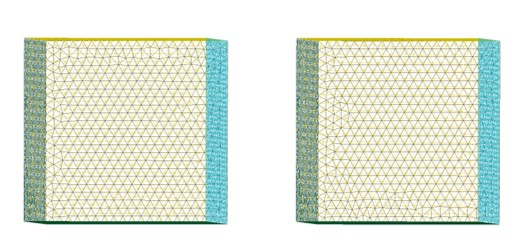
\includegraphics[scale = 0.5]{figures/merger_sponge_level0.jpg} }}
    \qquad
    \subfloat[Level 1 \\ $h_{\text{coarse}} = 0.1$: $\text{dim}(\mathsf{V}_{\mathrm{i}k}) = 3092$,  N\textsuperscript{\underline{o}} of elements on both grids $ = 6216$
    \\ $h_{\text{fine}} = 0.05$: $\text{dim}(\mathsf{V}_{\mathrm{i}k}) = 8510$,  N\textsuperscript{\underline{o}} of elements on both grids $ = 17052$]{{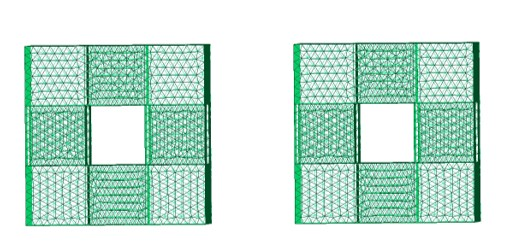
\includegraphics[width=0.4\textwidth]{figures/merger_sponge_level1.jpg} }}
    \qquad
    \subfloat[Level 2 \\ $h_{\text{coarse}} = 0.1$: $\text{dim}(\mathsf{V}_{\mathrm{i}k}) = 14464$,  N\textsuperscript{\underline{o}} of elements on both grids $ = 29568$
    \\ $h_{\text{fine}} = 0.05$: $\text{dim}(\mathsf{V}_{\mathrm{i}k}) = 27136$,  N\textsuperscript{\underline{o}} of elements on both grids $ = 54912$]{{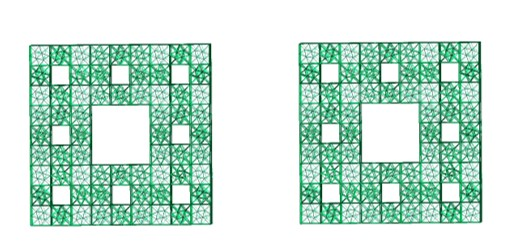
\includegraphics[width=0.5\textwidth]{figures/merger_sponge_level2.jpg} }}
    \caption{Menger sponges in different levels. The length of each sponge is 1.}
    \label{Menger sponges}
\end{figure}

\begin{table}[H]
    \centering
    \begin{tabular}{ |P{2cm}||p{2cm}|p{2cm}|p{2cm}|  }
        \hline
        \multicolumn{4}{|c|}{Normalized Casimir energy in two menger sponges' case} \\
        \hline
        Distance & Level 0 & Level 1 & Level 2\\
        \hline
        0.5   & 0.08350    & 0.08229     & 0.08112\\
        0.75  & 0.02737    & 0.02688     & 0.02670\\
        1.0   & 0.01305    & 0.01288     & 0.01282\\
        1.25  & 0.007357   & 0.007283    & 0.007252\\
        1.5   & 0.004607   & 0.004568    & 0.004551\\
        1.75  & 0.003099   & 0.003076    & 0.003065\\
        2.0   & 0.002195   & 0.002181    & 0.002174\\
        2.25  & 0.001618   & 0.001608    & 0.001603\\
        2.5   & 0.001230   & 0.001223    & 0.001220\\
        2.75  & 0.0009593  & 0.0009541   & 0.0009514\\
        3.0   & 0.0007638  & 0.0007598   & 0.0007577\\
        \hline
       \end{tabular}
       \caption{\label{Normalized Casimir energy in two menger sponges' case} Normalized Casimir energy in two menger sponges' case}
    \end{table}

\begin{figure}[H]
    \centering
    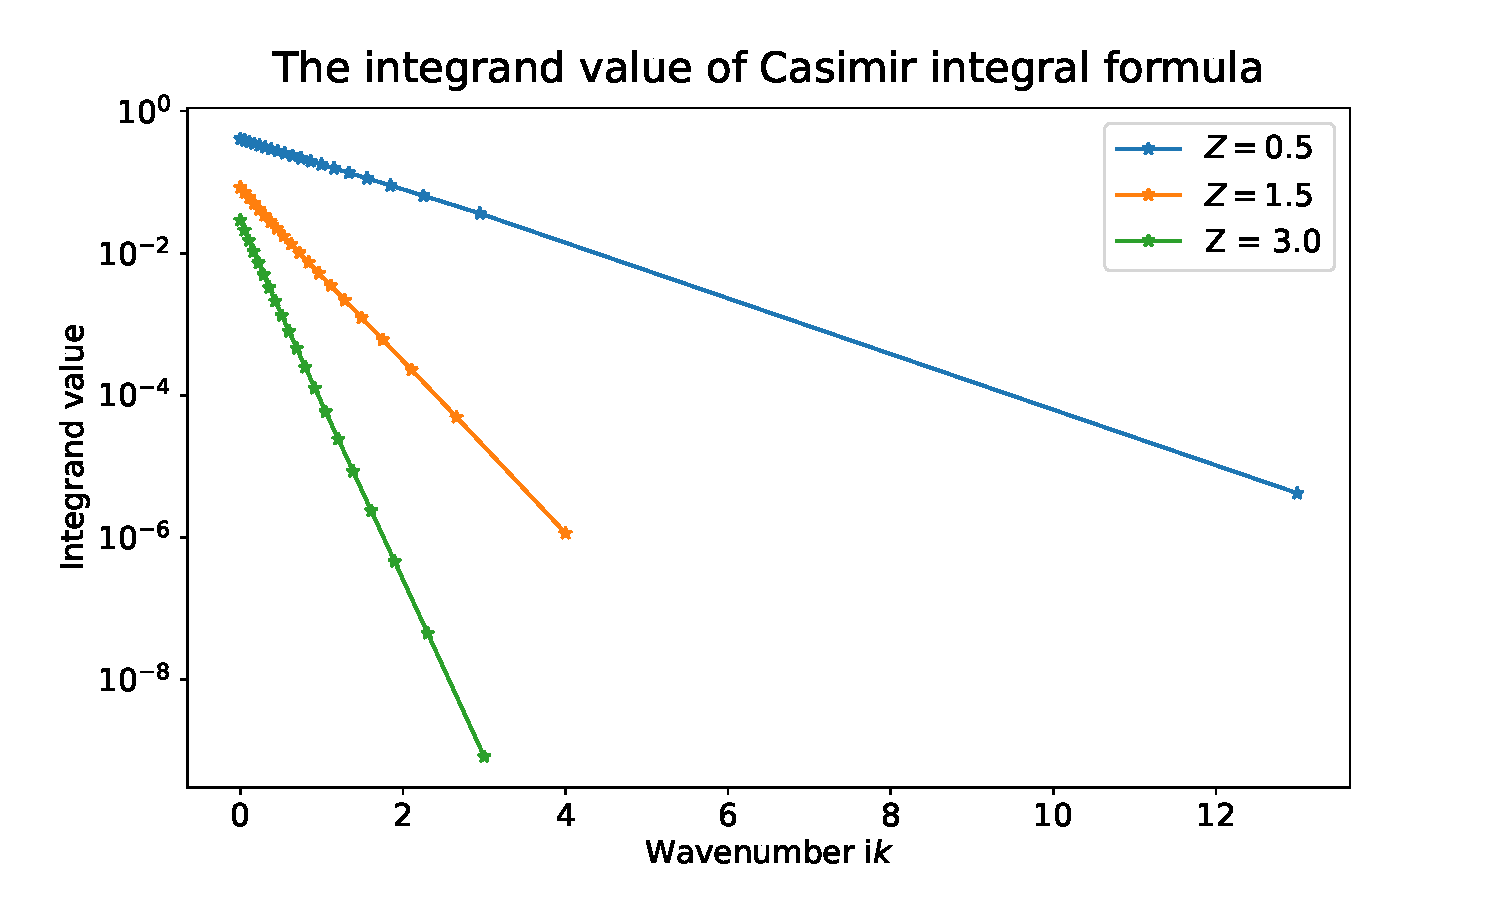
\includegraphics[scale = 1]{figures/level1_integrand_Value.png}
    \caption{The integrand of the Casimir energy between two menger sponges in Level 1 with distance $Z = 0.5$, 1.5 and 3.0.}
    \end{figure}

\begin{figure}[H]
        \centering
        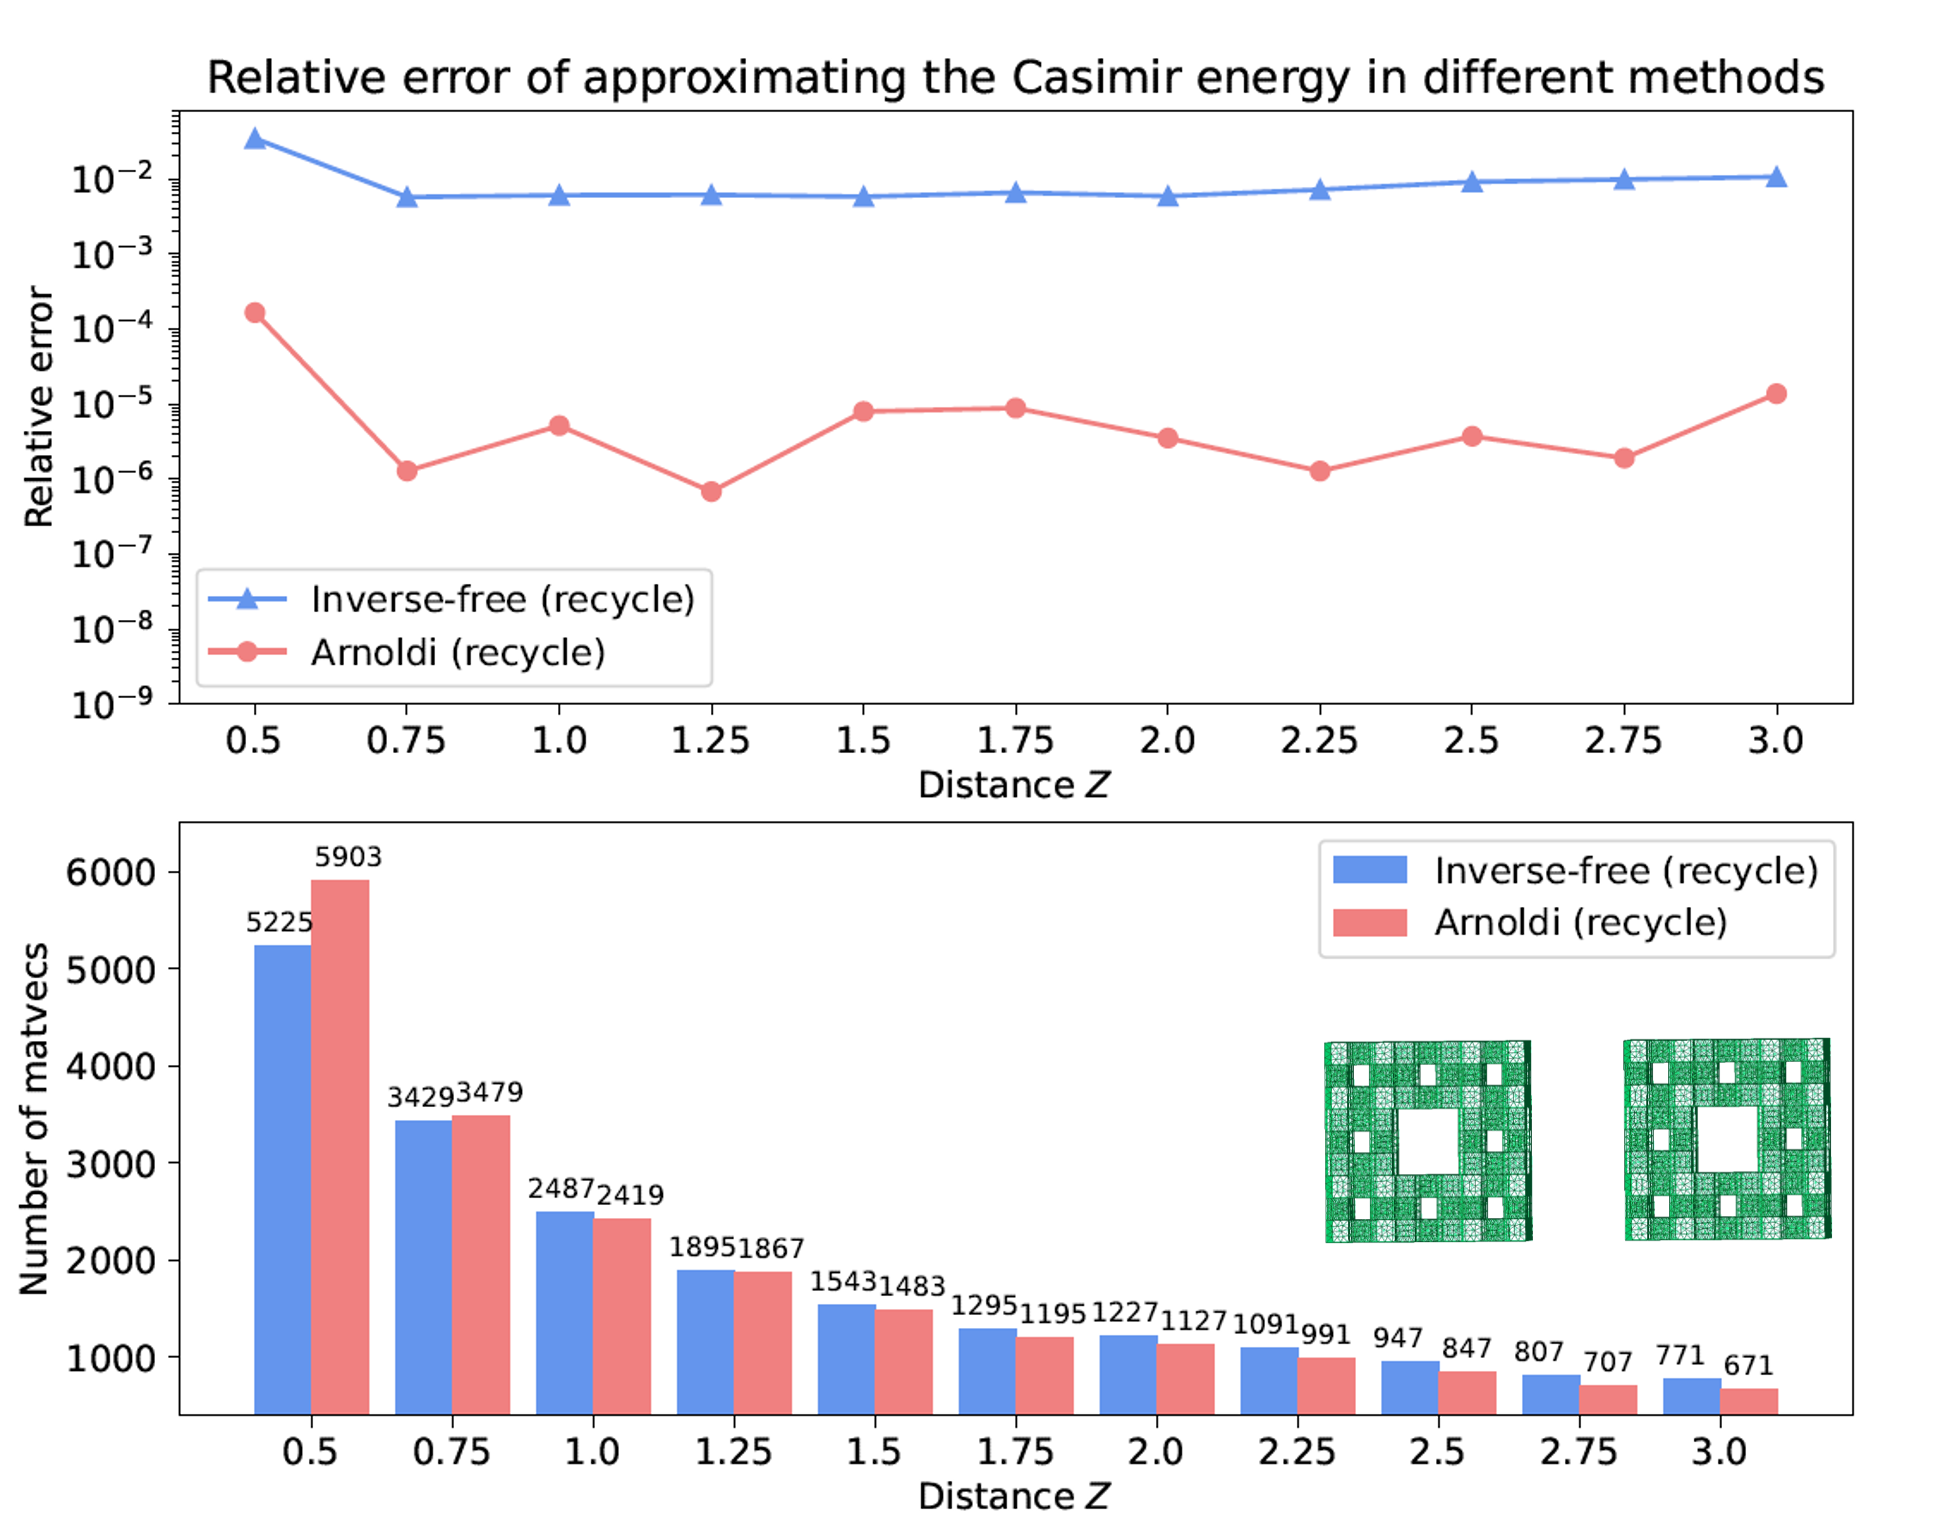
\includegraphics[scale = 1]{figures/level2_rel_err.png}
        \caption{Menger sponges in Level 2's case: relative distance between the reference value (computed by Richardson extrapolation) with the estimates evaluated from the standard Arnoldi 
        method with subspace recycled (solid red circles) and inverse-free Krylov subspace method 
        with subspace recycled (solid blue triangles). The dimension of the Krylov subspace is $m = 100$.}
\end{figure}


%==========================================================================================
In the next example, the scatterers are ice crystals with different number of branches ranging from 2 to 6 (see Figure \ref{Ice crystals with different number of branches}).

%By Figure \ref{Normalized Casimir energy in ice crystals' case}, when the number of branches increases from 2 to 4, the Casimir energy increases as expected. But 
%when the branches number added up to 5 and 6, the Casimir energy is much smaller since the main cross-sectional part cannot be as close as the 
%2, 3, 4-branches cases. 

\begin{figure}[H]
    \begin{subfigure}{0.3\linewidth}
        \centering
        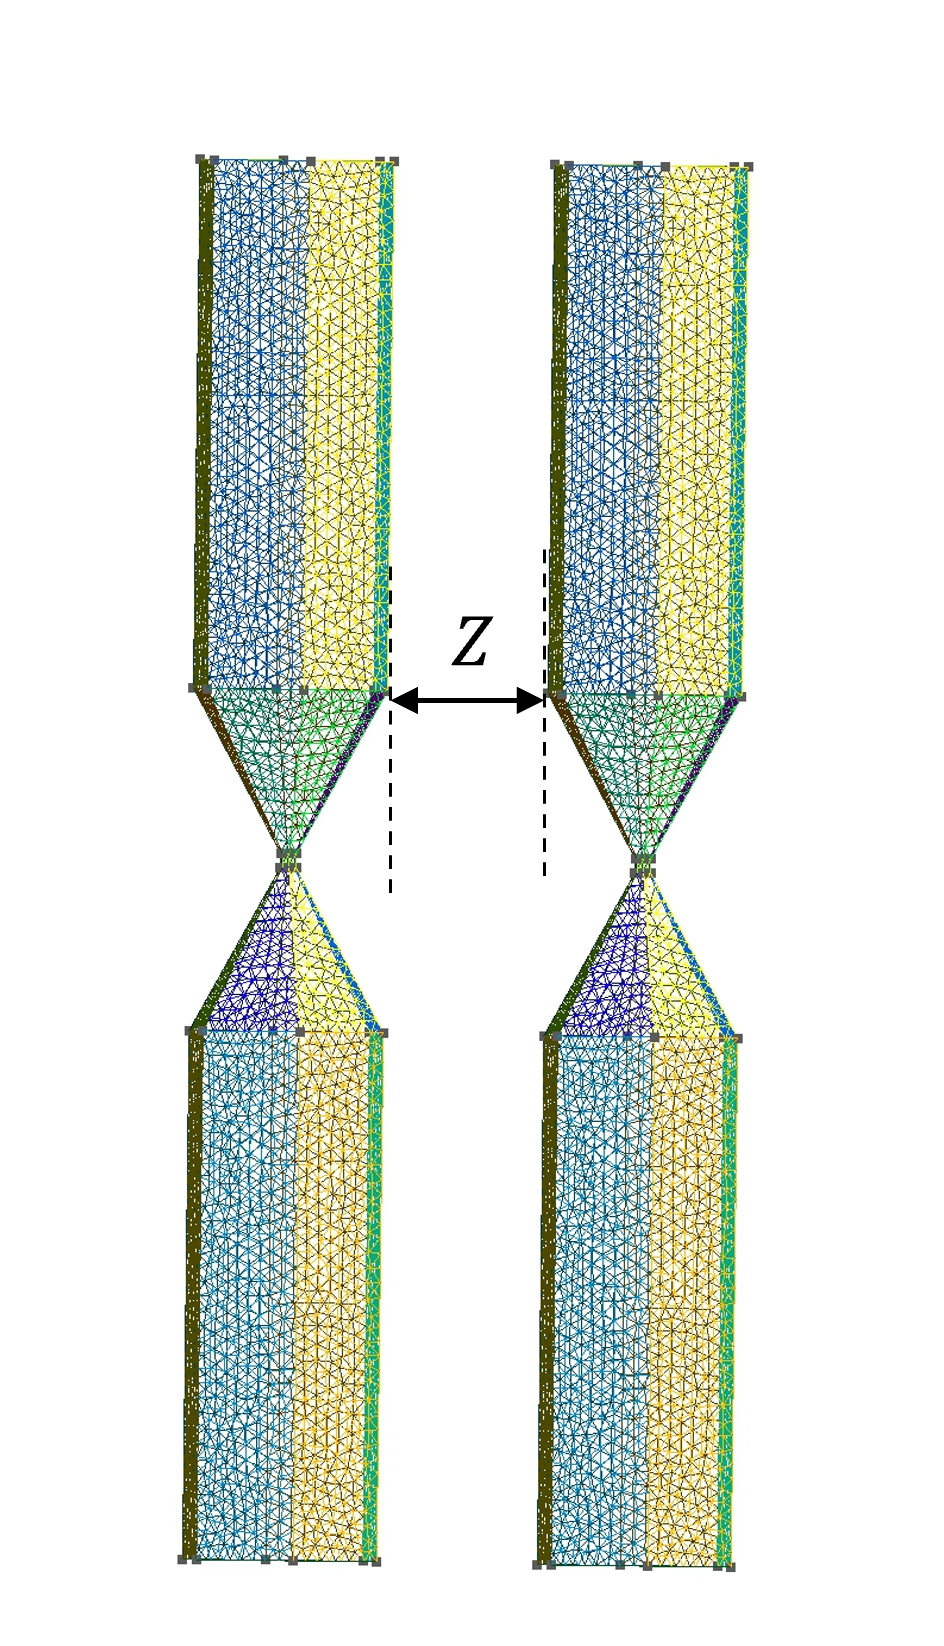
\includegraphics[scale = 0.4]{figures/2branches}
        \caption{Two branches: $\text{dim}(\mathsf{V}_{\mathrm{i}k}) = 8792$ \newline N\textsuperscript{\underline{o}} of elements on both grids $ = 17576$}
        \end{subfigure}
        \begin{subfigure}{0.3\linewidth}
            \centering
            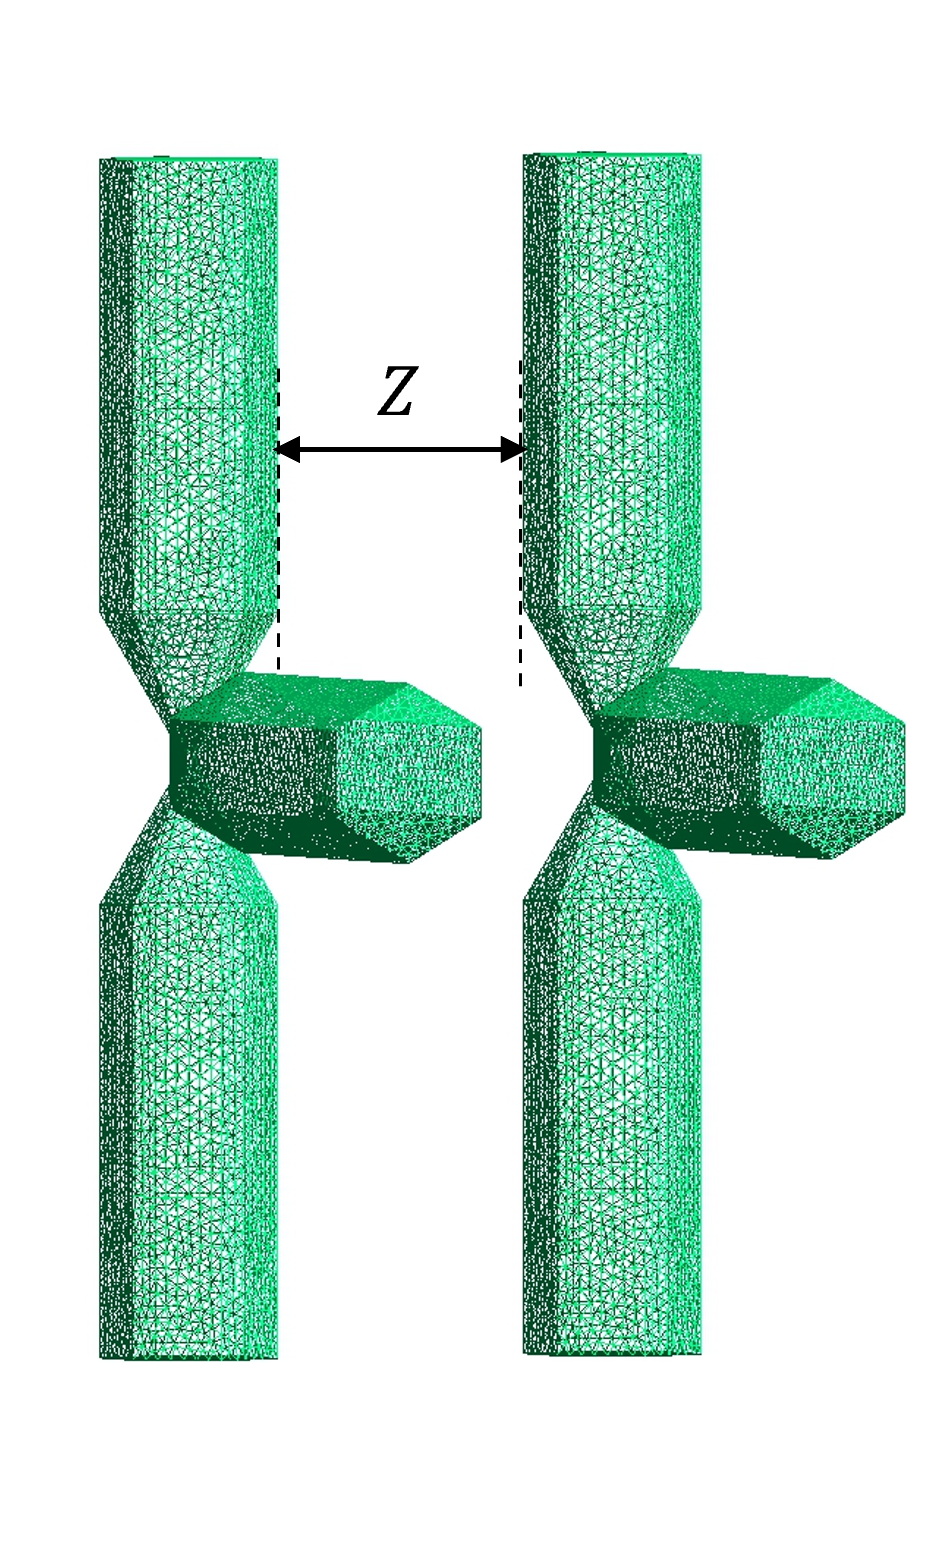
\includegraphics[scale = 0.4]{figures/3branches}
            \caption{Three branches: $\text{dim}(\mathsf{V}_{\mathrm{i}k}) = 13104$ \newline N\textsuperscript{\underline{o}} of elements on both grids $ = 26200$}
            \end{subfigure}
            \begin{subfigure}{0.3\linewidth}
                \centering
                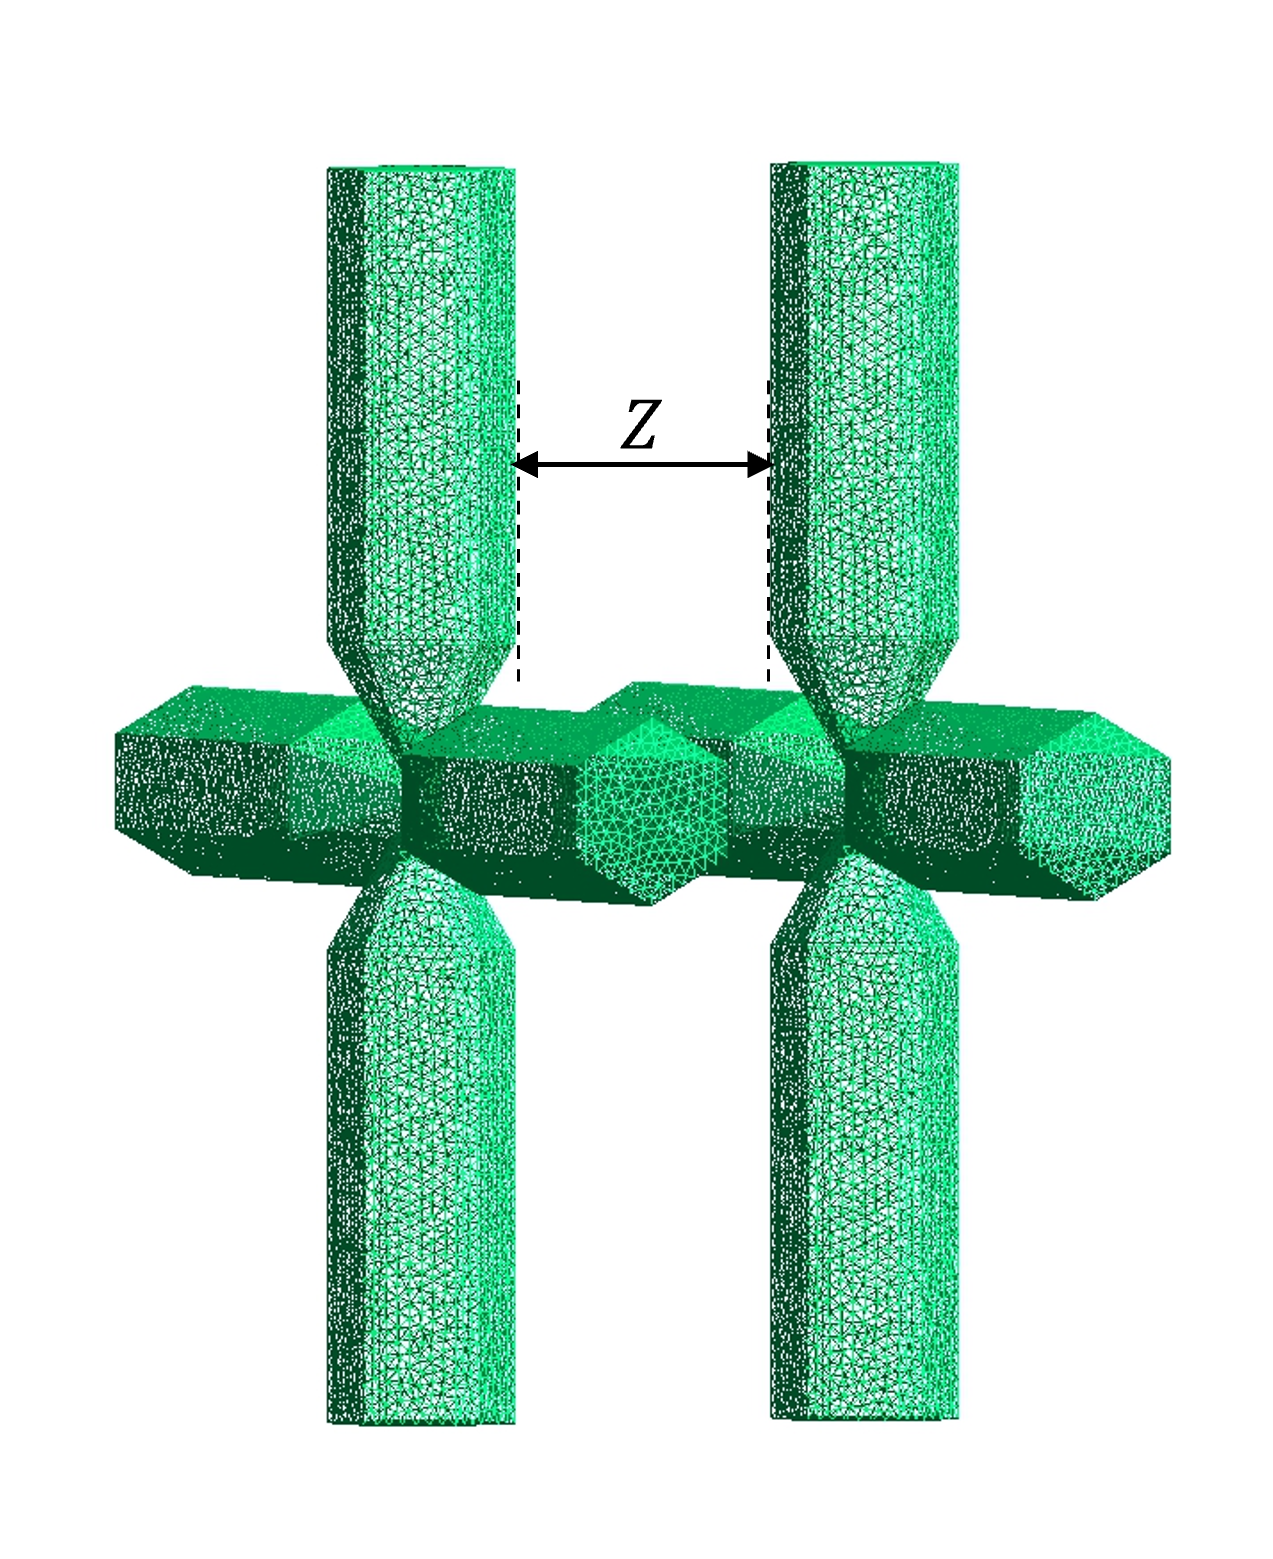
\includegraphics[scale = 0.4]{figures/4branches}
                \caption{Four branches: $\text{dim}(\mathsf{V}_{\mathrm{i}k}) = 17554$ \newline N\textsuperscript{\underline{o}} of elements on both grids $ = 35100$}
                \end{subfigure}\\[1ex]
    %\begin{subfigure}{.5\linewidth}
    \centering
    \captionsetup[subfigure]{oneside,margin={0.4cm,0cm}}
    \subfloat[Five branches: $\text{dim}(\mathsf{V}_{\mathrm{i}k}) = 21950$ \newline N\textsuperscript{\underline{o}} of elements on both grids $ = 43900$]{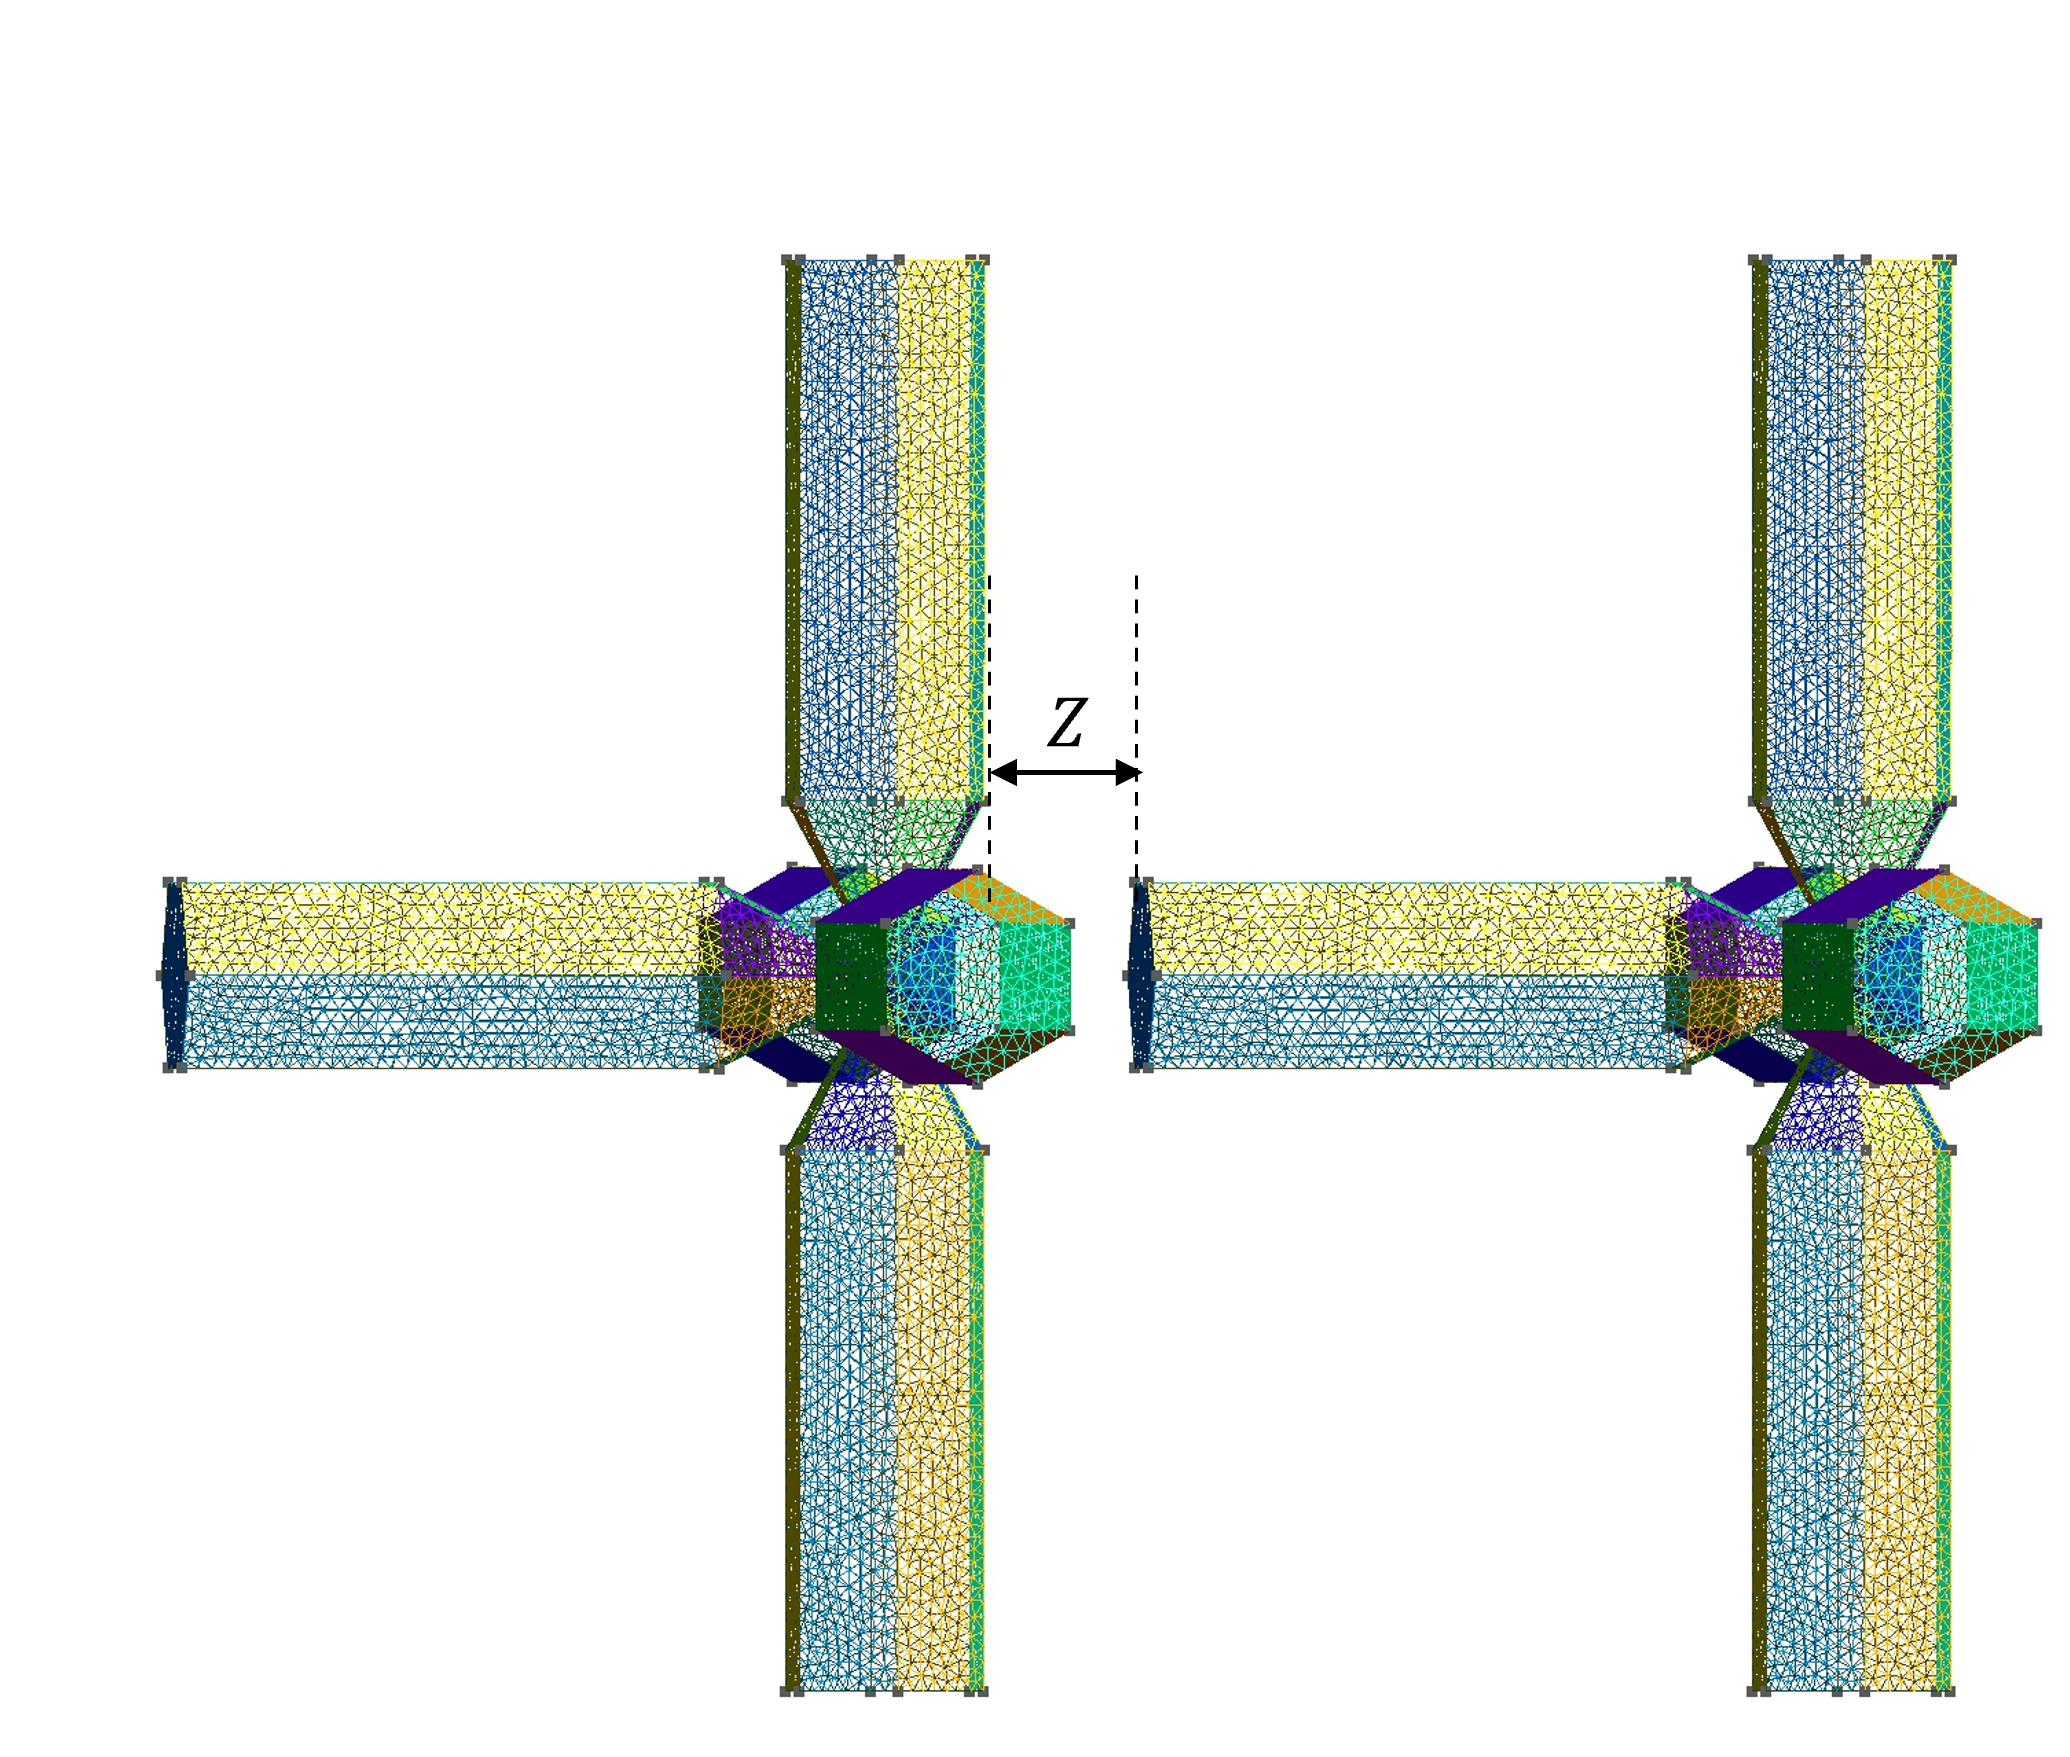
\includegraphics[scale=0.4]{figures/5branches}}
    %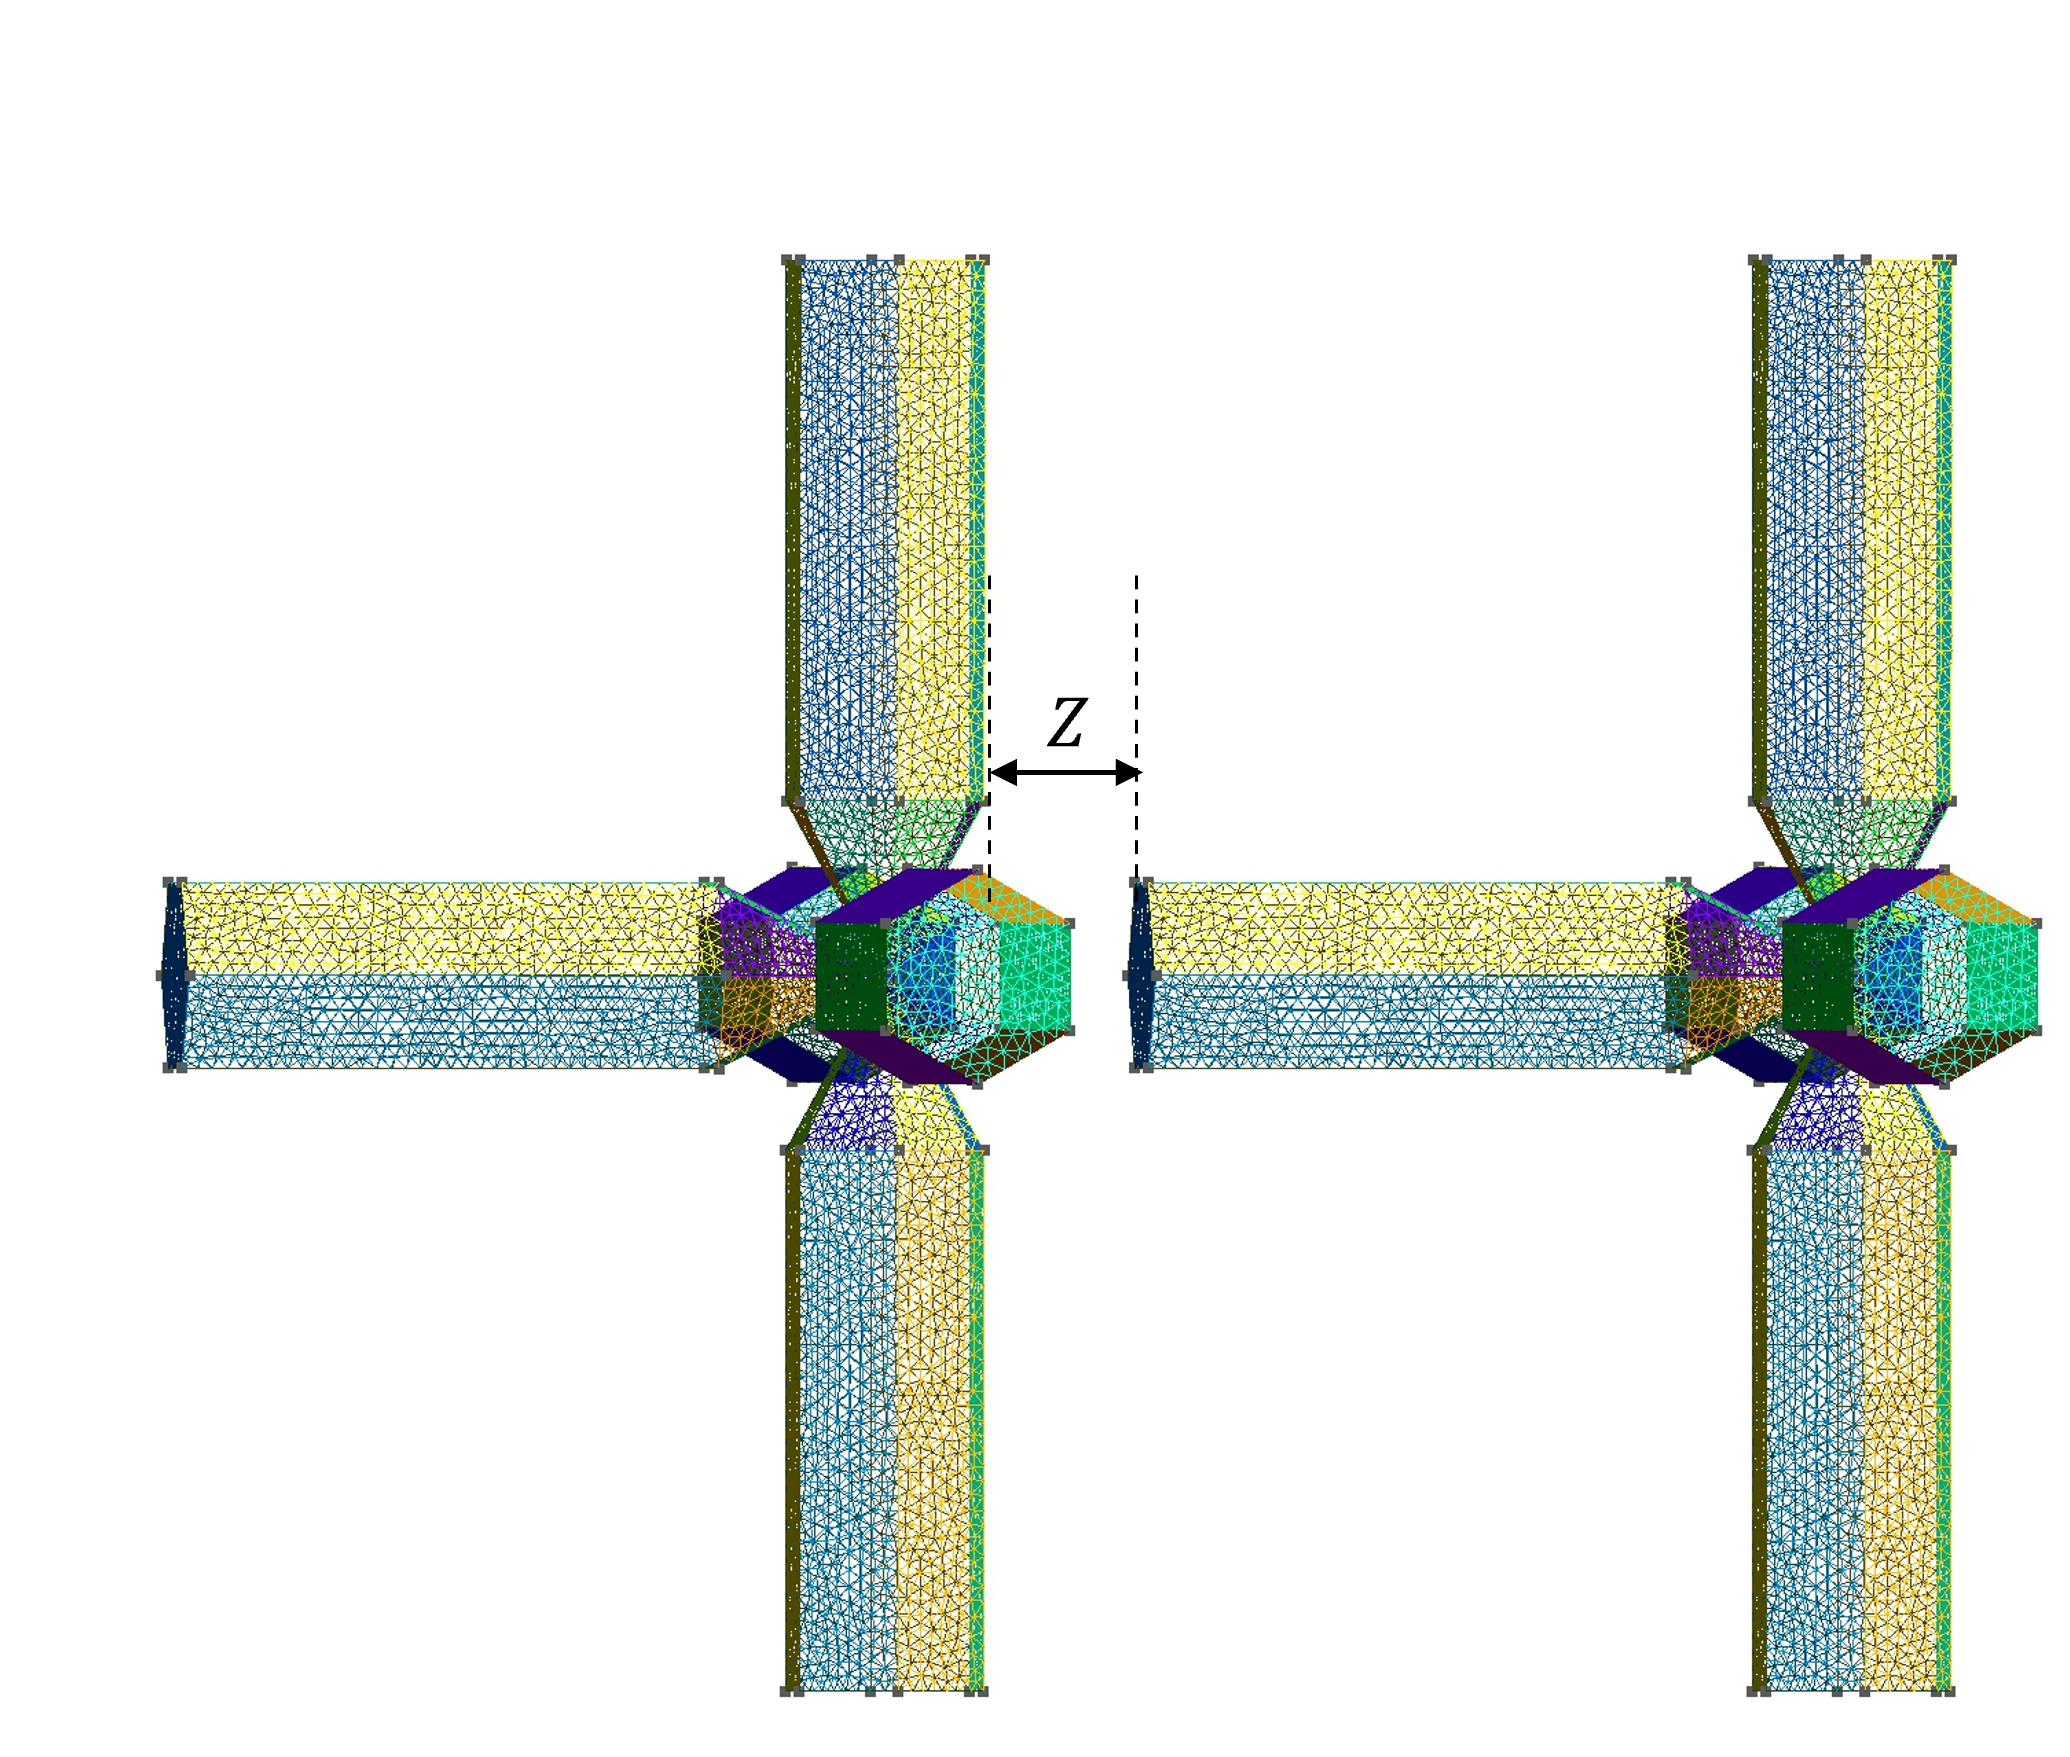
\includegraphics[scale = 0.4]{figures/5branches}
    %\caption{Five branches: $\text{dim}(\mathsf{V}_{\mathrm{i}k}) = 21950$ \newline N\textsuperscript{\underline{o}} of elements on both grids $ = 43900$}
    %\end{subfigure}%
    %\begin{subfigure}{.5\linewidth}
    \centering
    %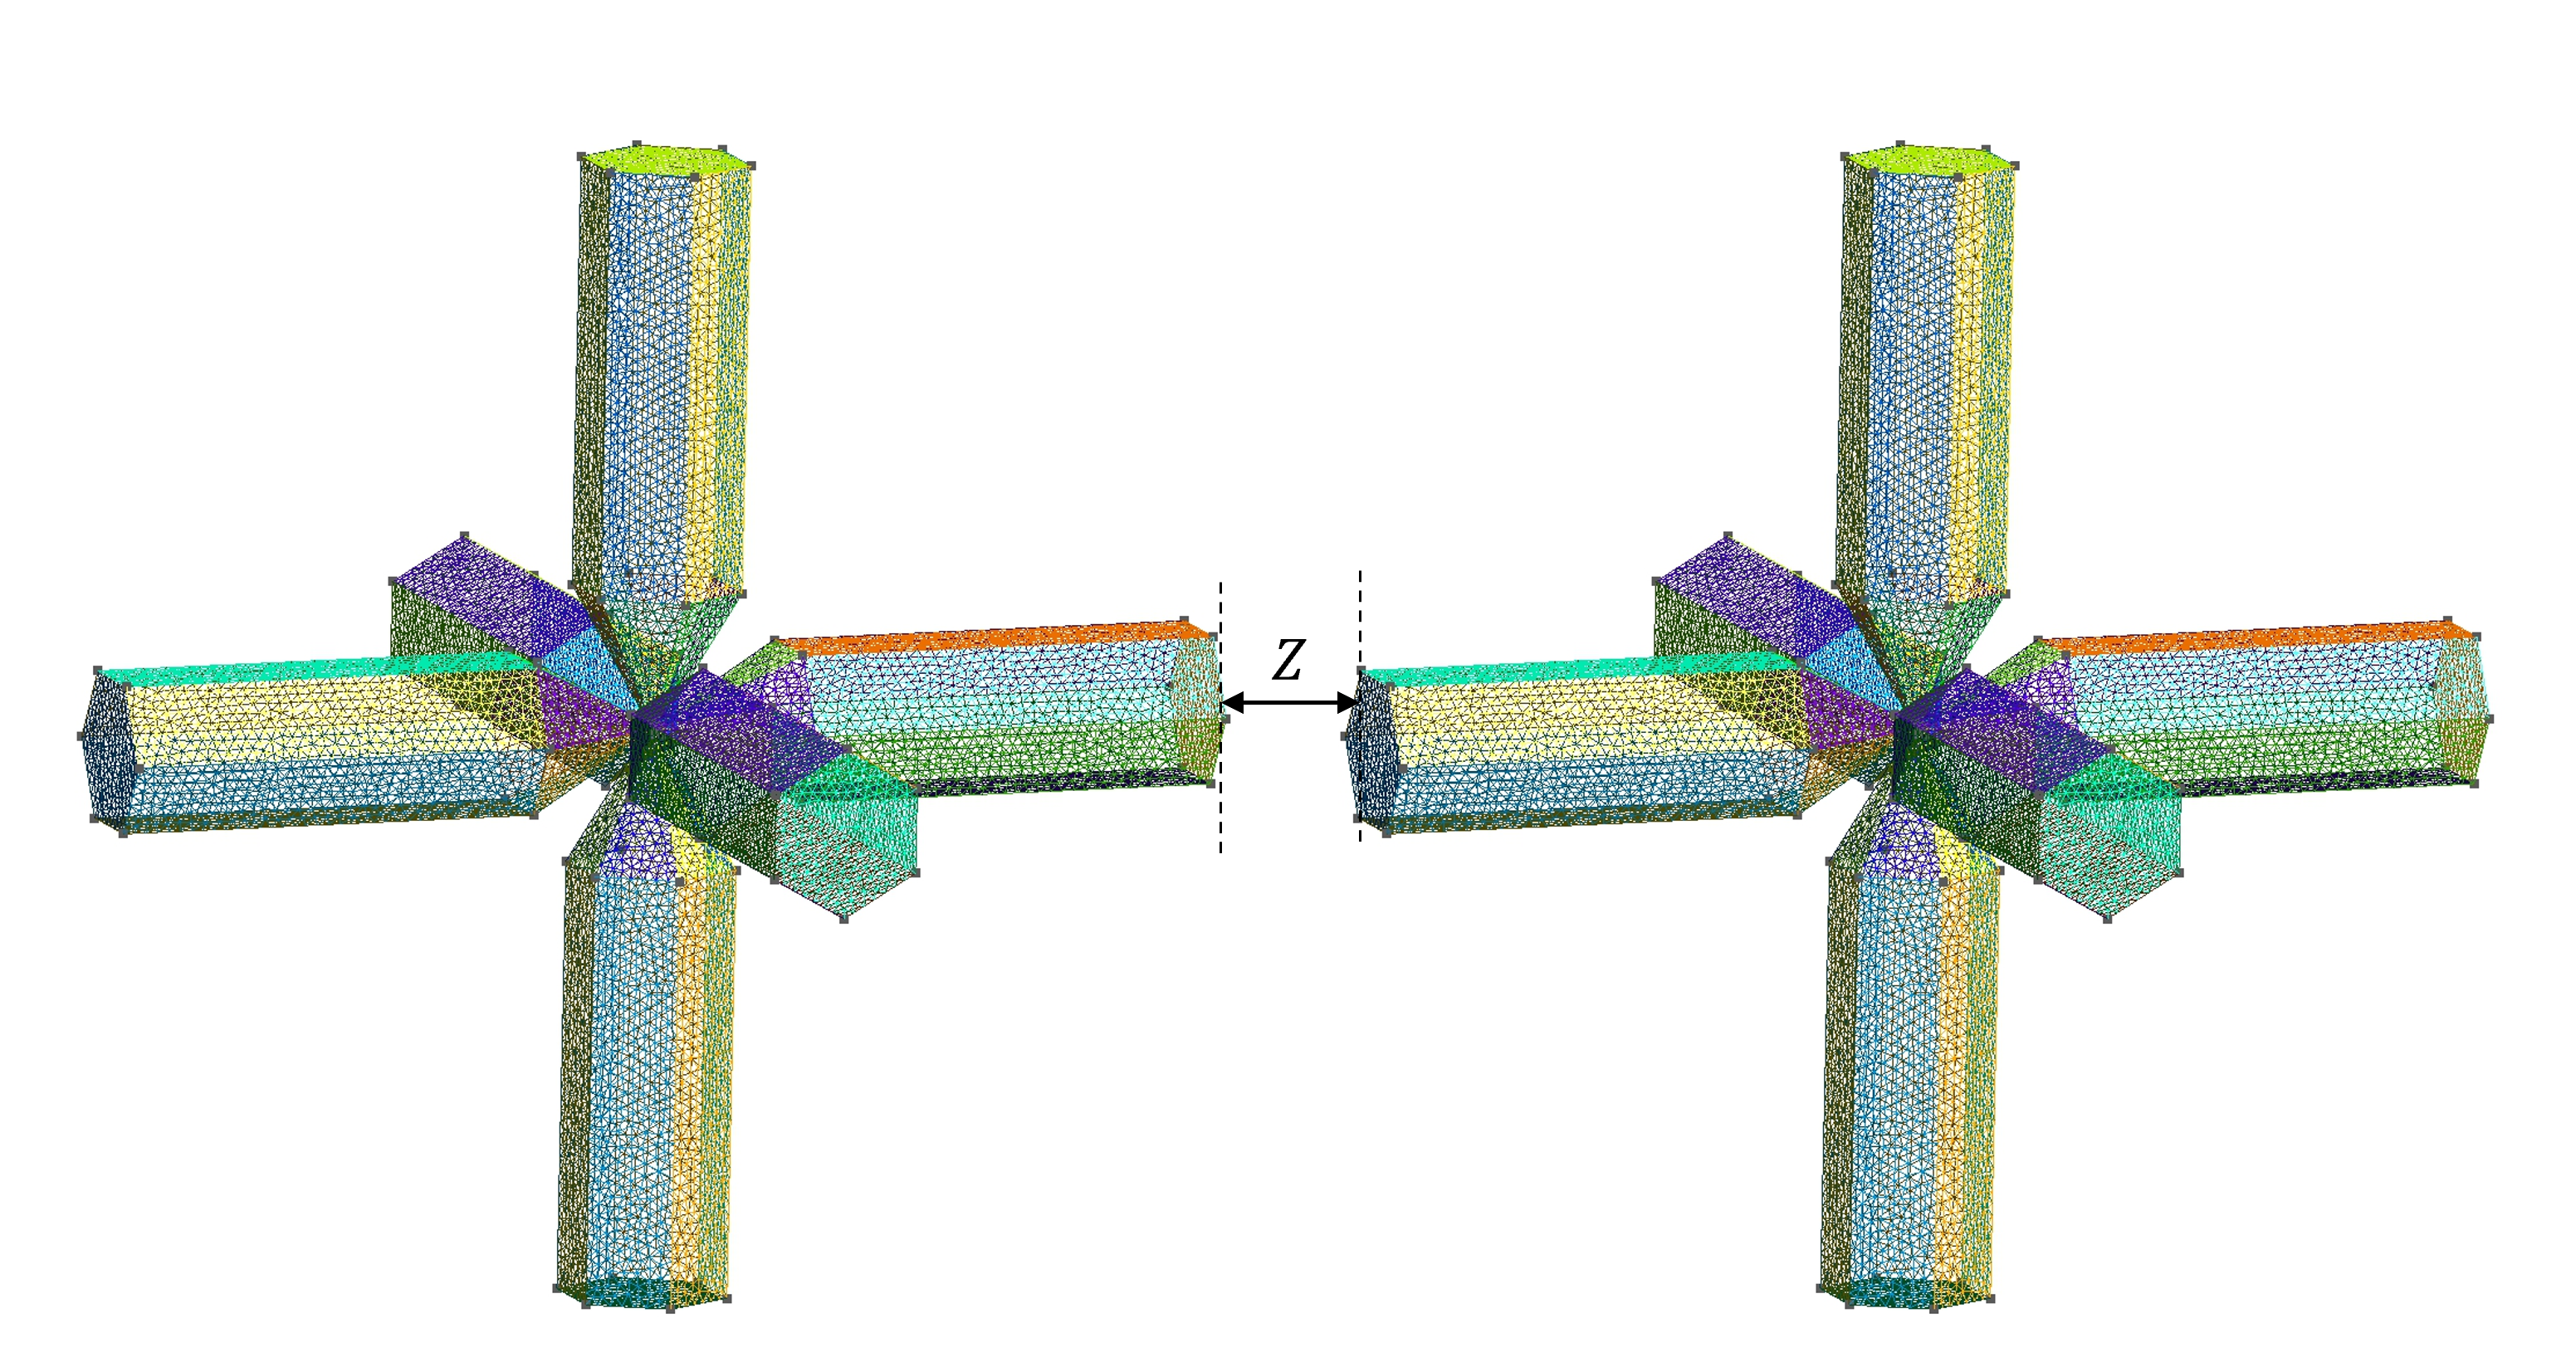
\includegraphics[scale = 0.4]{figures/6branches}
    %\caption{Six branches: $\text{dim}(\mathsf{V}_{\mathrm{i}k}) = 26262$ \newline N\textsuperscript{\underline{o}} of elements on both grids $ = 52556$}
    %\end{subfigure}
    \hspace*{1.5cm}
    \captionsetup[subfigure]{oneside,margin={1.2cm,0cm}}
    \subfloat[Six branches: $\text{dim}(\mathsf{V}_{\mathrm{i}k}) = 26262$ \newline N\textsuperscript{\underline{o}} of elements on both grids $ = 52556$]{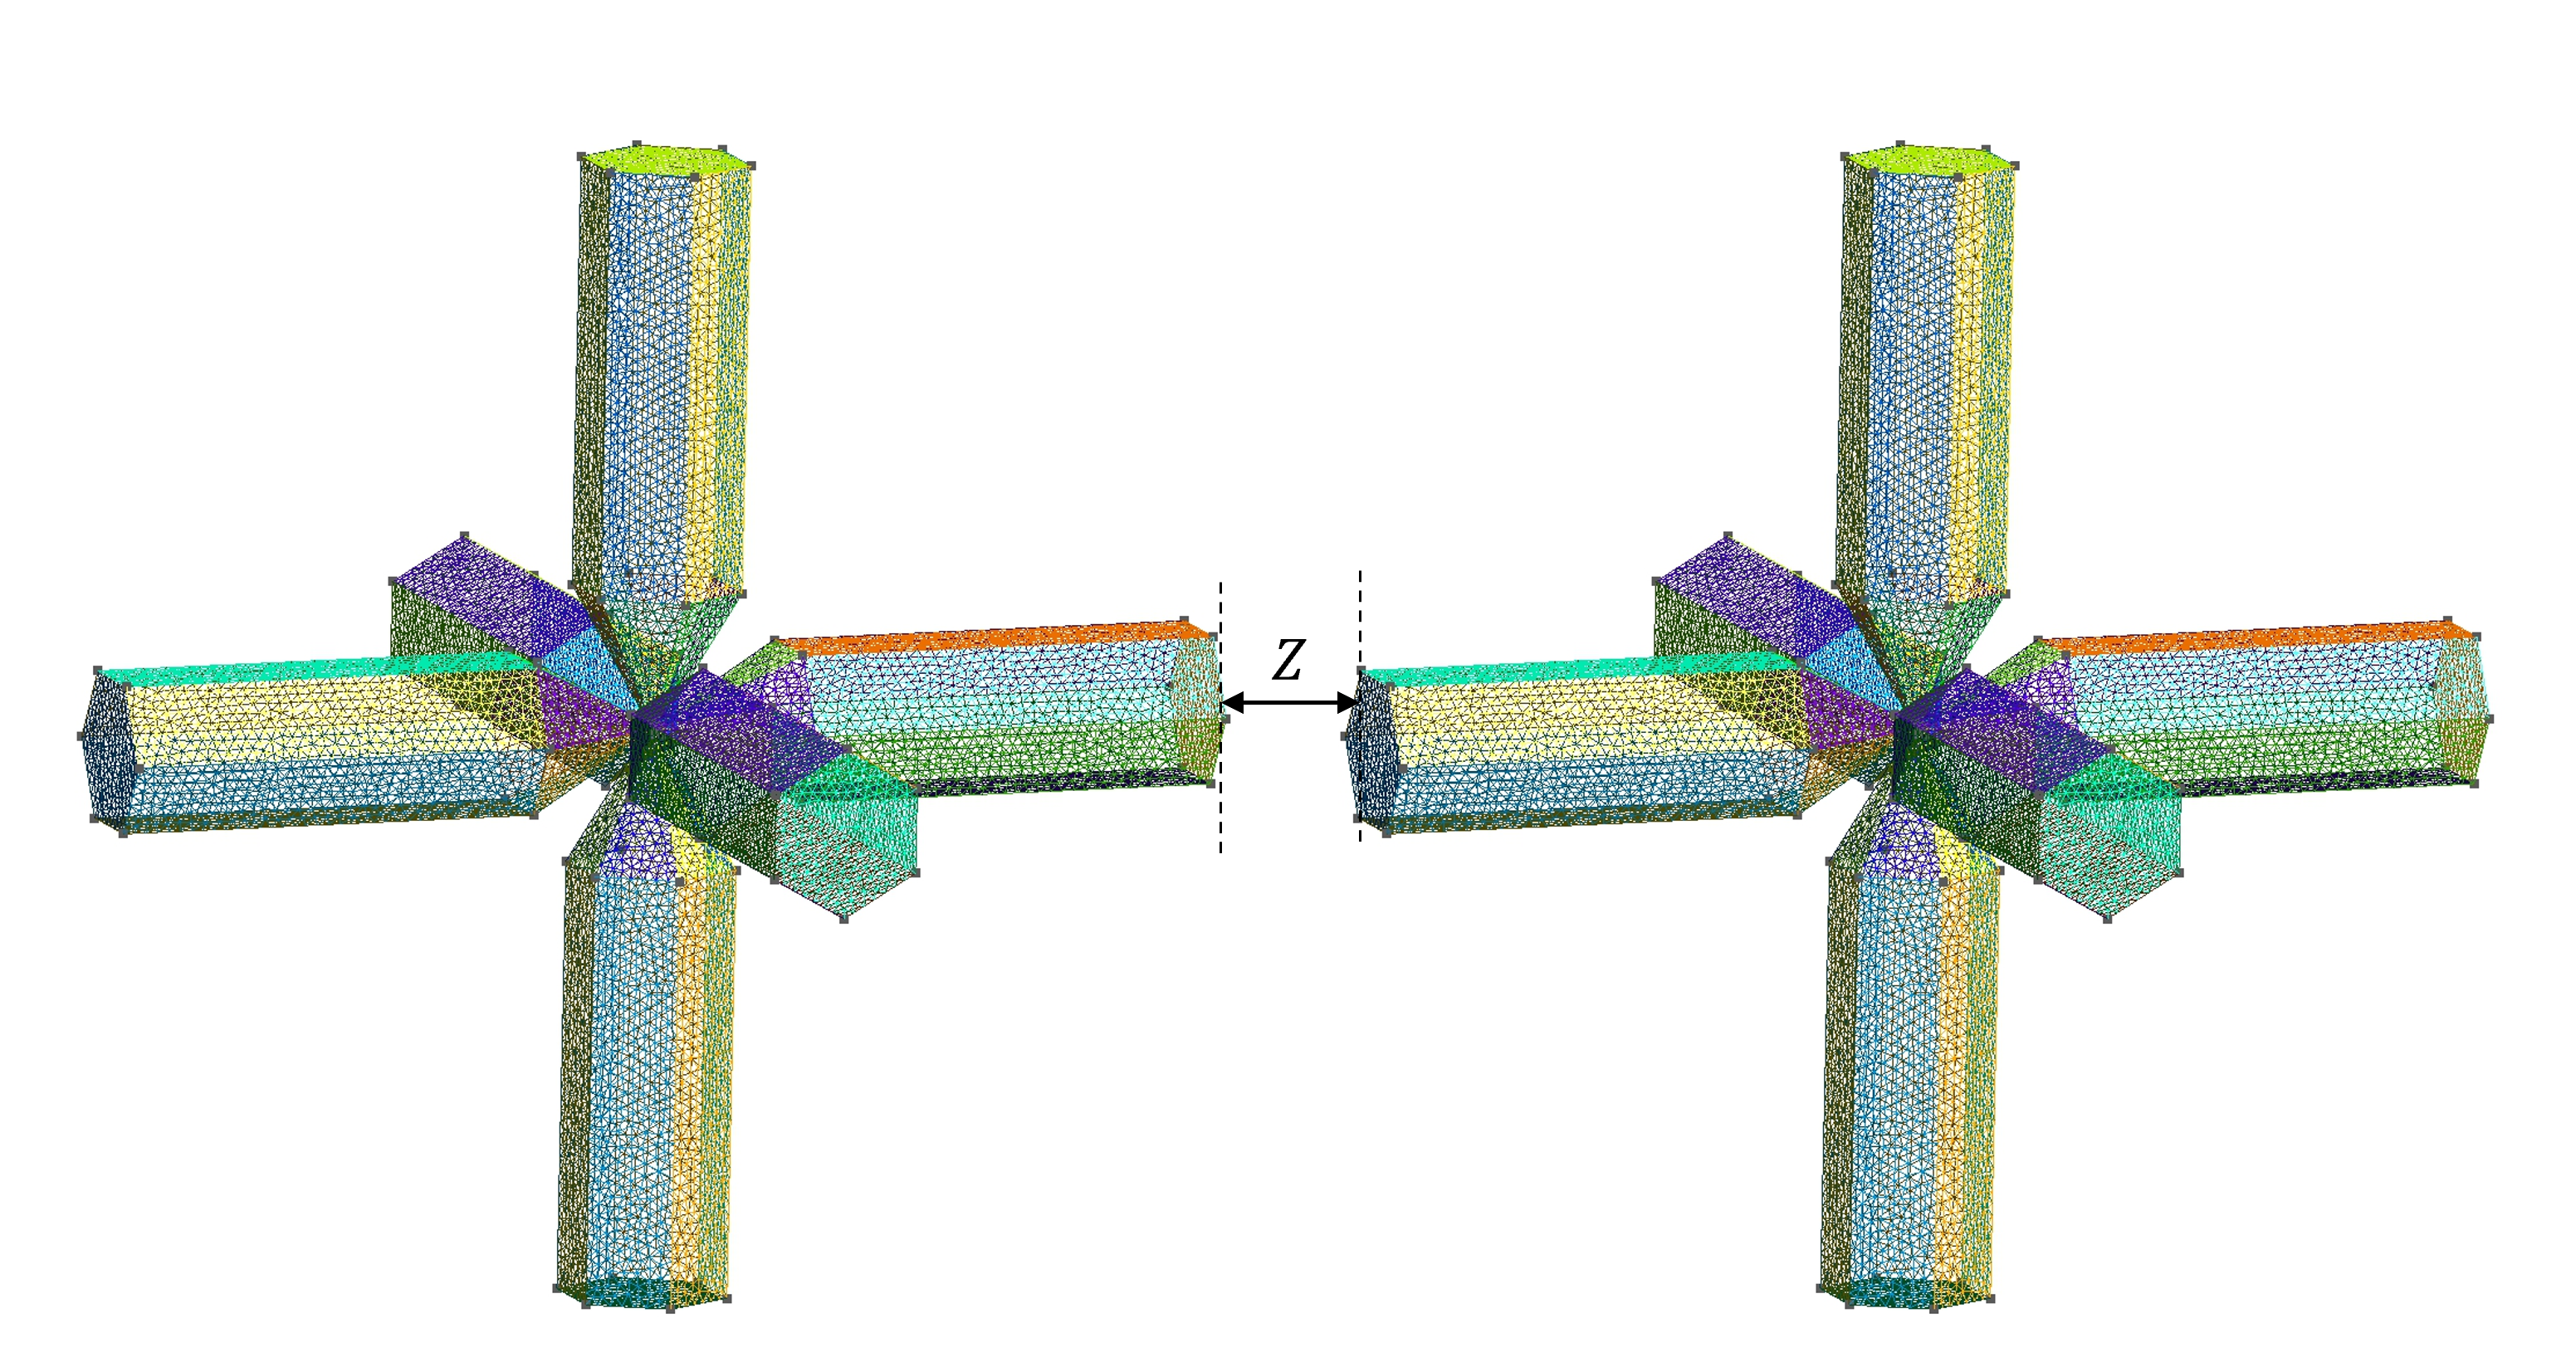
\includegraphics[scale=0.4]{figures/6branches}}
    \caption{Ice crystals with different number of branches}
    \label{Ice crystals with different number of branches}
    \end{figure}

    \begin{table}[H]
        \centering
        \begin{tabular}{ |P{2cm}||p{2cm}|p{2cm}|p{2cm}|p{2cm}|p{2cm}|  }
            \hline
            \multicolumn{6}{|c|}{Normalized Casimir energy in ice crystals' case} \\
            \hline
            Distance & 2-branches & 3-branches & 4-branches & 5-branches & 6-branches\\
            \hline
            0.5   & 0.04112    & 0.05989    & 0.07848   & 0.07873    & 0.01128\\
            0.75  & 0.01499    & 0.02184    & 0.02855   & 0.02873    & 0.005017\\
            1.0   & 0.007403   & 0.01080    & 0.01412   & 0.01428    & 0.002965\\
            1.25  & 0.004242   & 0.006198   & 0.008113  & 0.008242   & 0.001985\\
            1.5   & 0.002672   & 0.003905   & 0.005117  & 0.005223   & 0.001427\\
            1.75  & 0.001797   & 0.002624   & 0.003442  & 0.003530   & 0.001074\\
            2.0   & 0.001268   & 0.001849   & 0.002428  & 0.002501   & 0.0008357\\
            2.25  & 0.0009288  & 0.001353   & 0.001776  & 0.001839   & 0.0006664\\
            2.5   & 0.0007007  & 0.001019   & 0.001338  & 0.001391   & 0.0005410\\
            2.75  & 0.0005413  & 0.0007863  & 0.001033  & 0.001078   & 0.0004469\\
            3.0   & 0.0004270  & 0.0006188  & 0.0008134 & 0.0008526  & 0.0003741\\
            \hline
           \end{tabular}
           \caption{\label{Normalized Casimir energy in ice crystals' case table} Normalized Casimir energy in 2- to 6-branched ice crystals' case}
        \end{table}

        \begin{figure}[H]
            \centering
            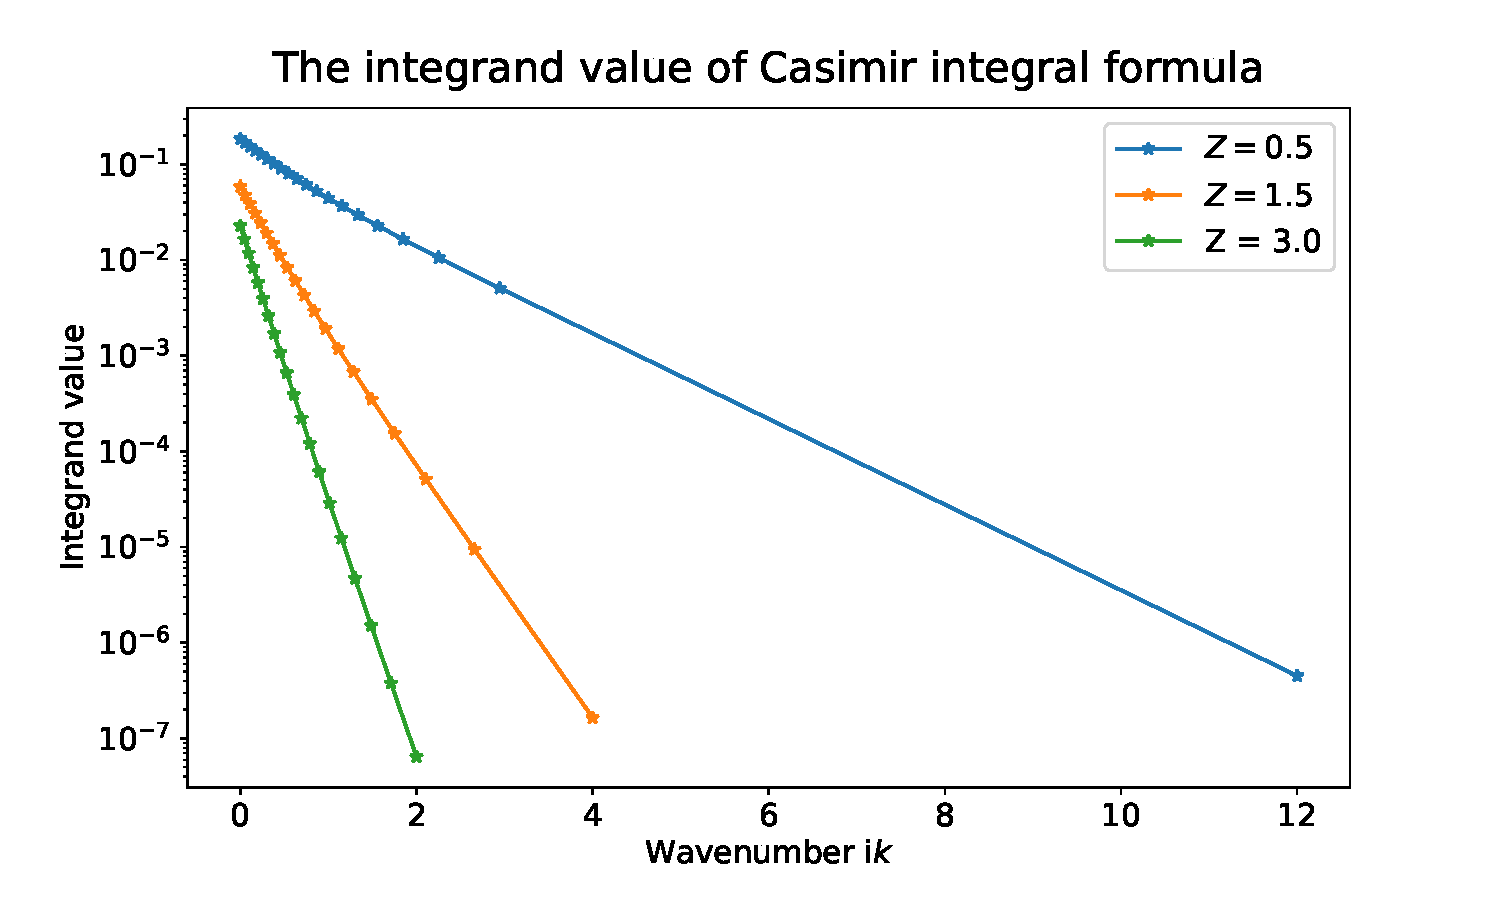
\includegraphics[scale = 1]{figures/5branches_integrand_Value.png}
            \caption{The integrand of the Casimir energy between two five-branches ice crystals with distance $Z = 0.5$, 1.5 and 3.0.}      
              \end{figure}
        
        \begin{figure}[H]
                \centering
                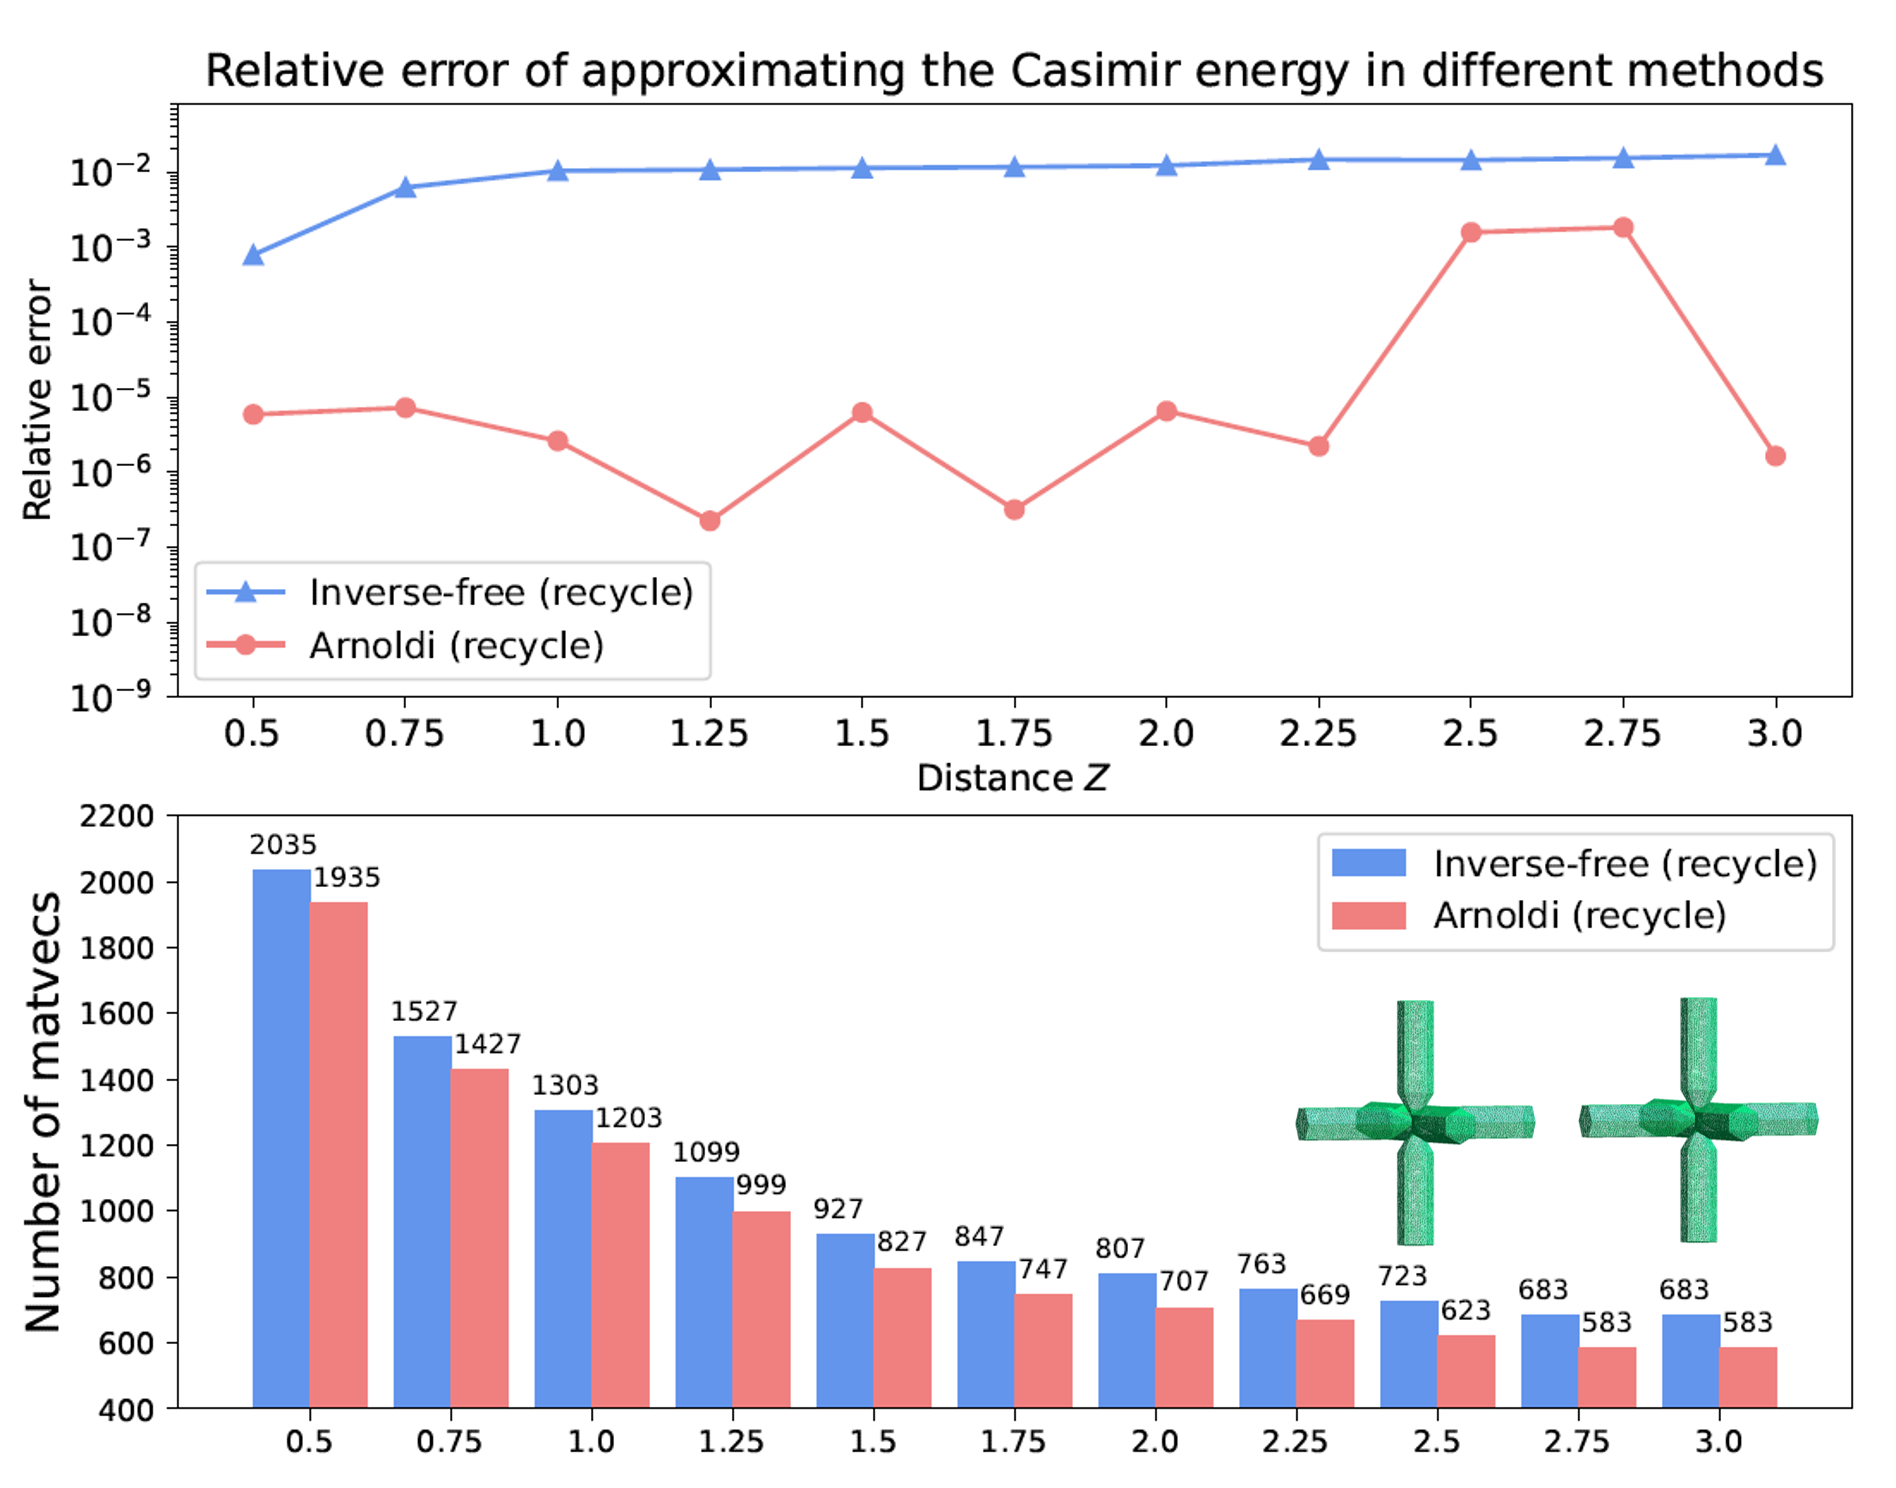
\includegraphics[scale = 1]{figures/6branches_rel_err.png}
                \caption{Six-branches ice crystals' case: relative distance between the reference value (computed by Richardson extrapolation) with the estimates evaluated from the standard Arnoldi 
                method with subspace recycled (solid red circles) and inverse-free Krylov subspace method with subspace recycled (solid blue triangles). The dimension of the Krylov subspace is $m = 100$.}       
             \end{figure}

        
        %==================================================================================================
It is not hard to imagine that the Casimir energy would be different after the scatterers rotate while keeping the distance between them unchanged. Therefore, 
in the last example, we would see how the Casimir energy between two identical ellipsoids changes as one of the ellipsoids rotates.

In Figure \ref{Without rotation}, the above ellipsoid is centering at $(0,0,0)$ and the below one is centering at $(0, 0, -(0.5+0.5+Z))$, where $Z$ is the 
distance between these two ellipsoids. Without rotation, the Casimir energy between them with different distance $Z$ is plotted in Figure 
\ref{Casimir energy between two ellipsoids with different distances}.

To explore how the rotation affects the change of the Casimir energy, one can always keep one ellipsoid fixed and rotate the other one. The Figure 
\ref{Rotation around z-axis} and \ref{Rotation around x-axis} describe the case when one of the ellipsoids rotates around $z-$ and $x-$axis, respectively.
From the Figure \ref{Casimir energy when one of the ellipsoids rotates}, the Casimir energy changes periodically since we rotate one ellipsoid around 
$z-$ or $x-$axis by 360 degrees. 


\begin{figure}[H]
    \begin{subfigure}{\linewidth}
        \centering
        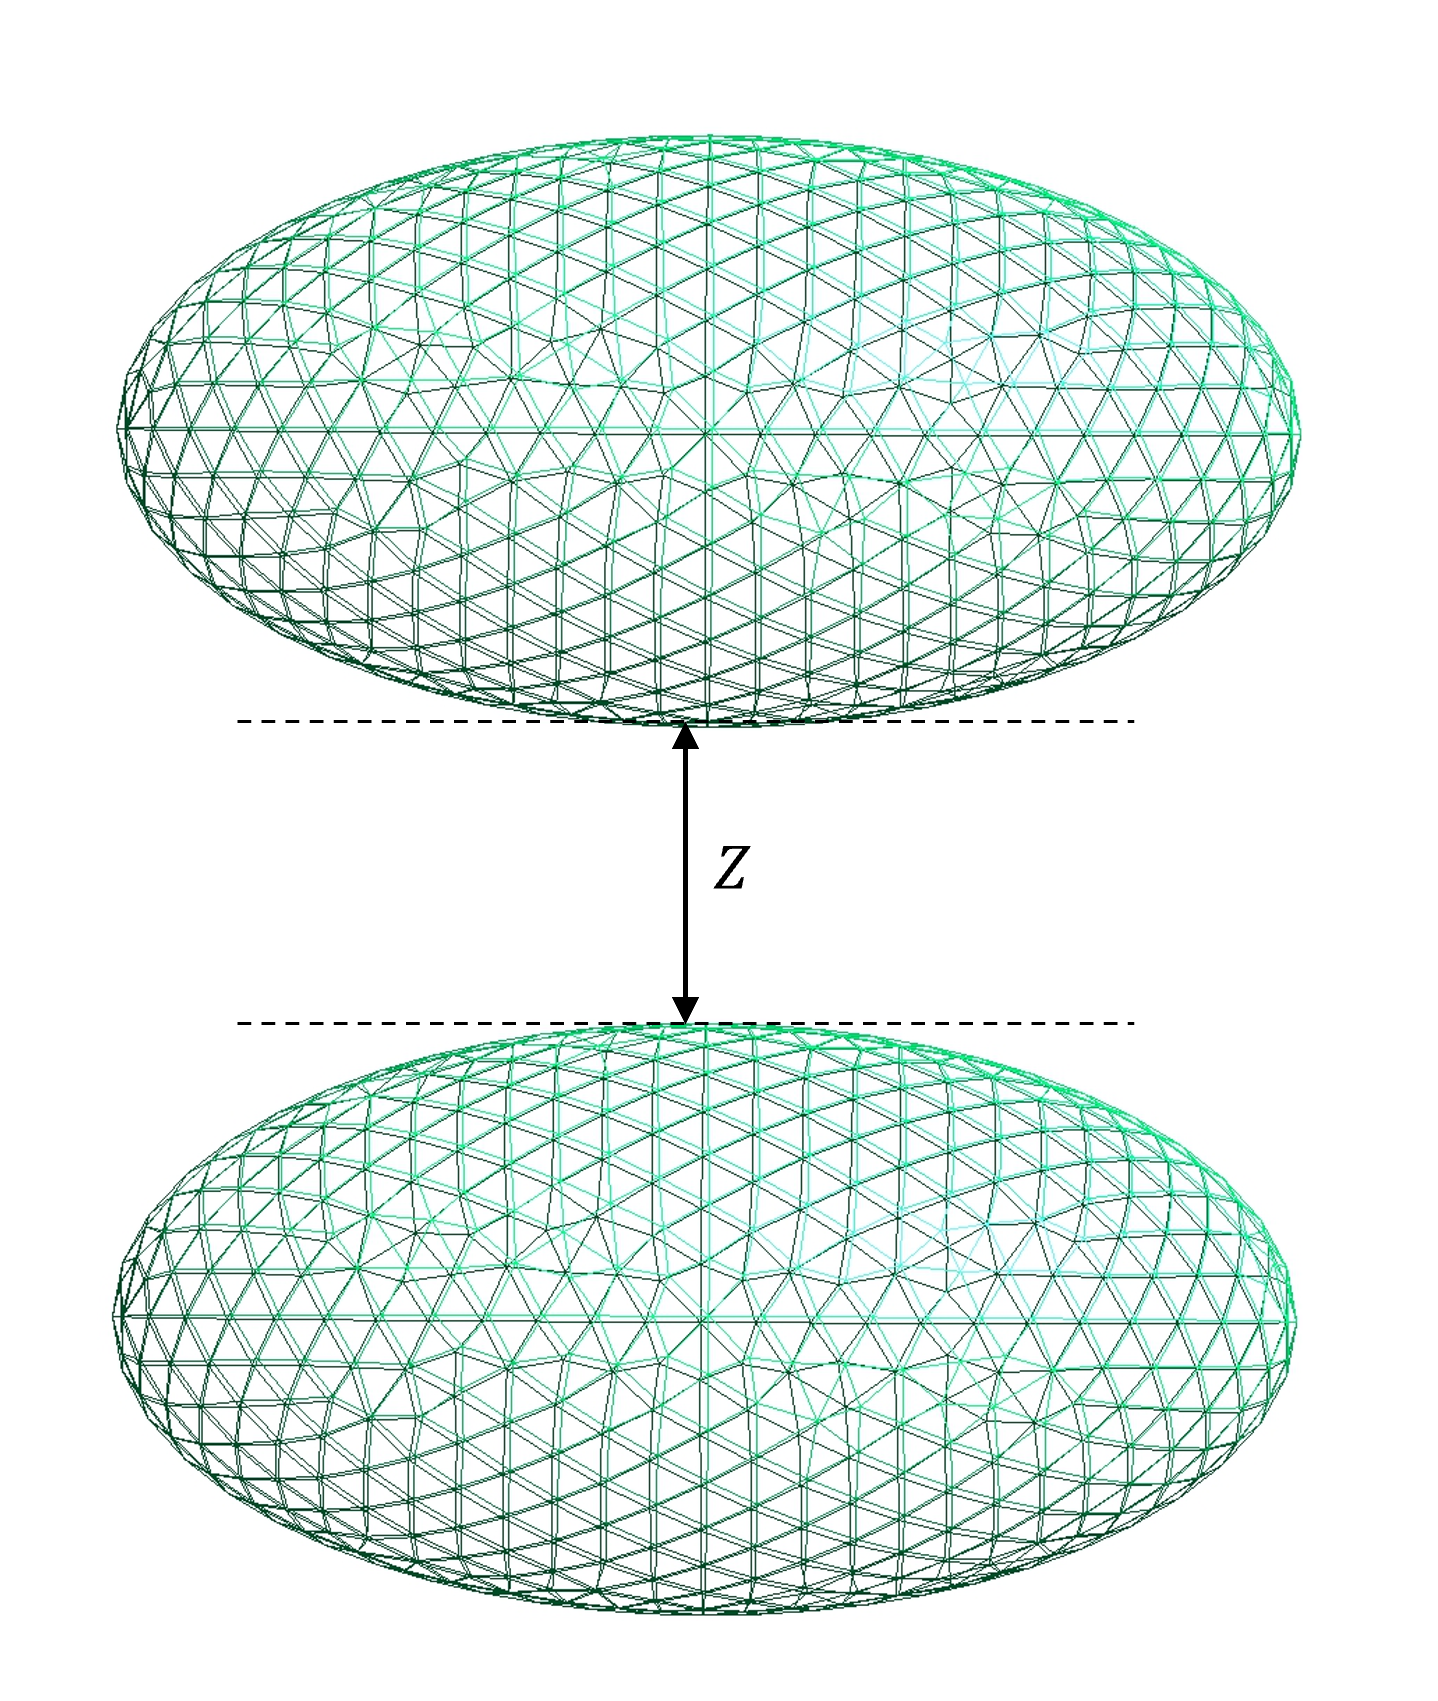
\includegraphics[scale = 0.3]{figures/two_ellipsoids}
        \caption{Without rotation}
        \label{Without rotation}
        \end{subfigure}\\[1ex]
    \begin{subfigure}[t]{.5\linewidth}
    \centering
    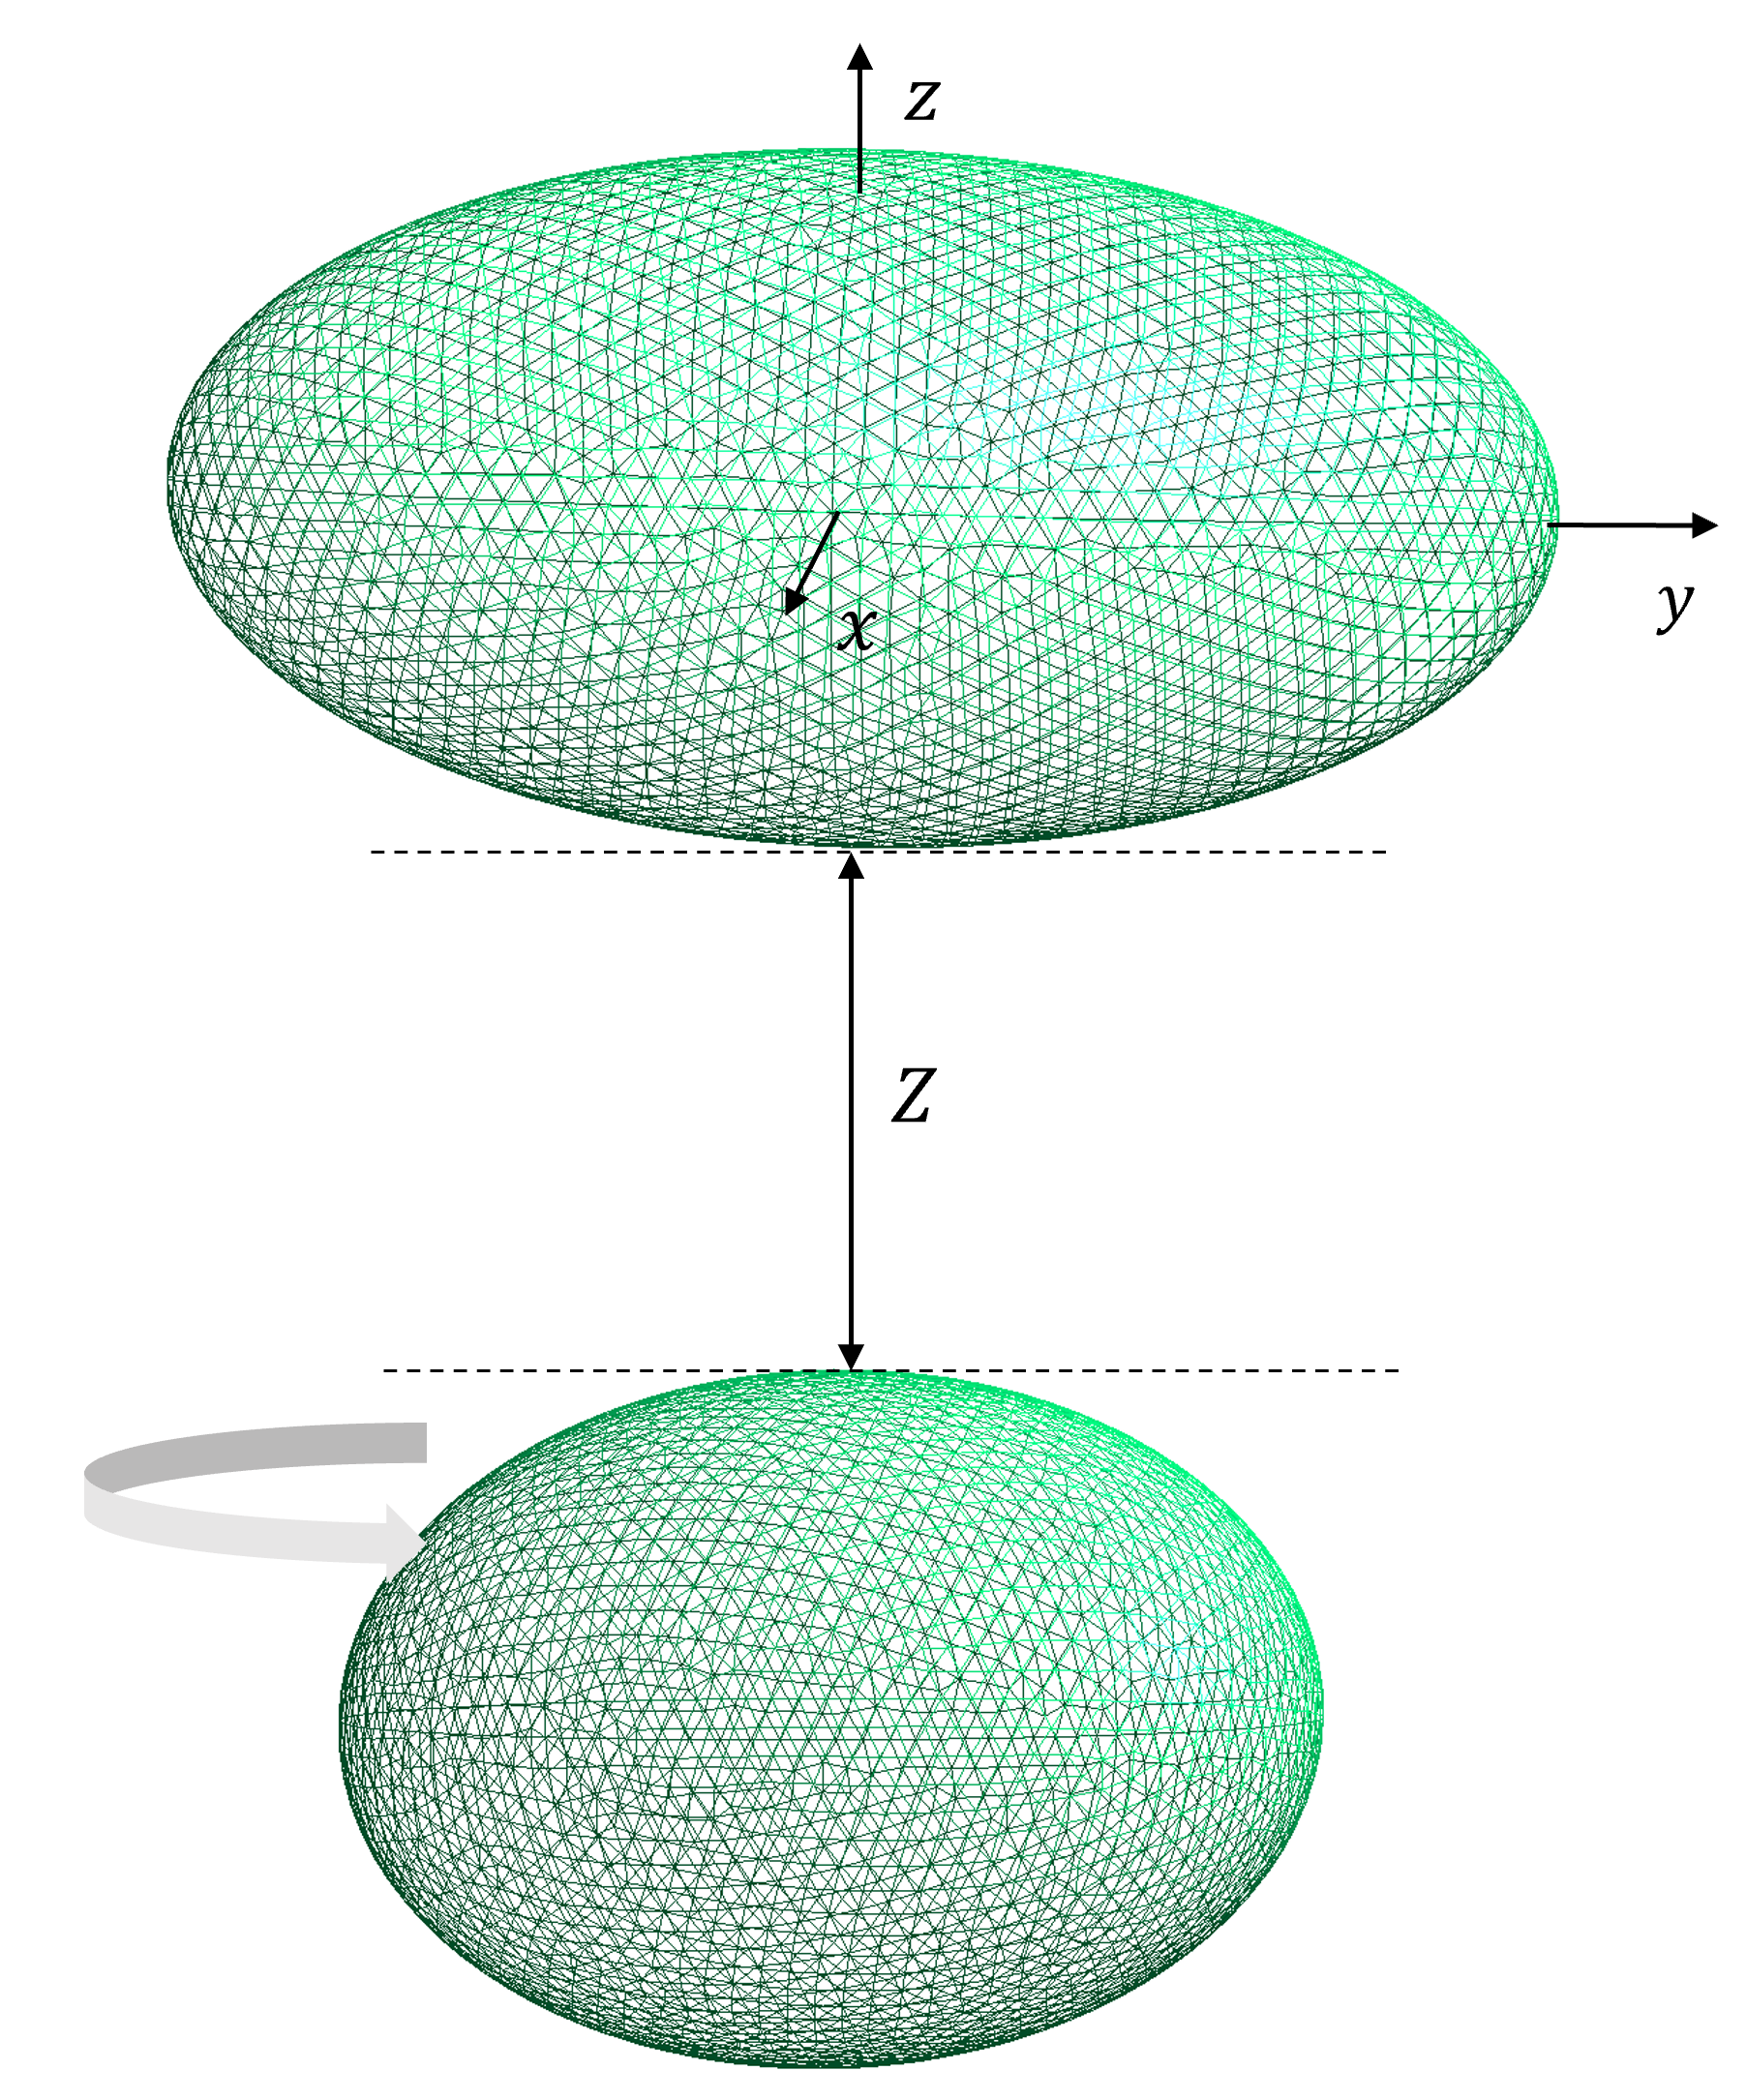
\includegraphics[scale = 0.3]{figures/Ellipsoid_z_axis}
    \caption{Rotation around z-axis}
    \label{Rotation around z-axis}
    \end{subfigure}%
    \begin{subfigure}[t]{.5\linewidth}
    \centering
    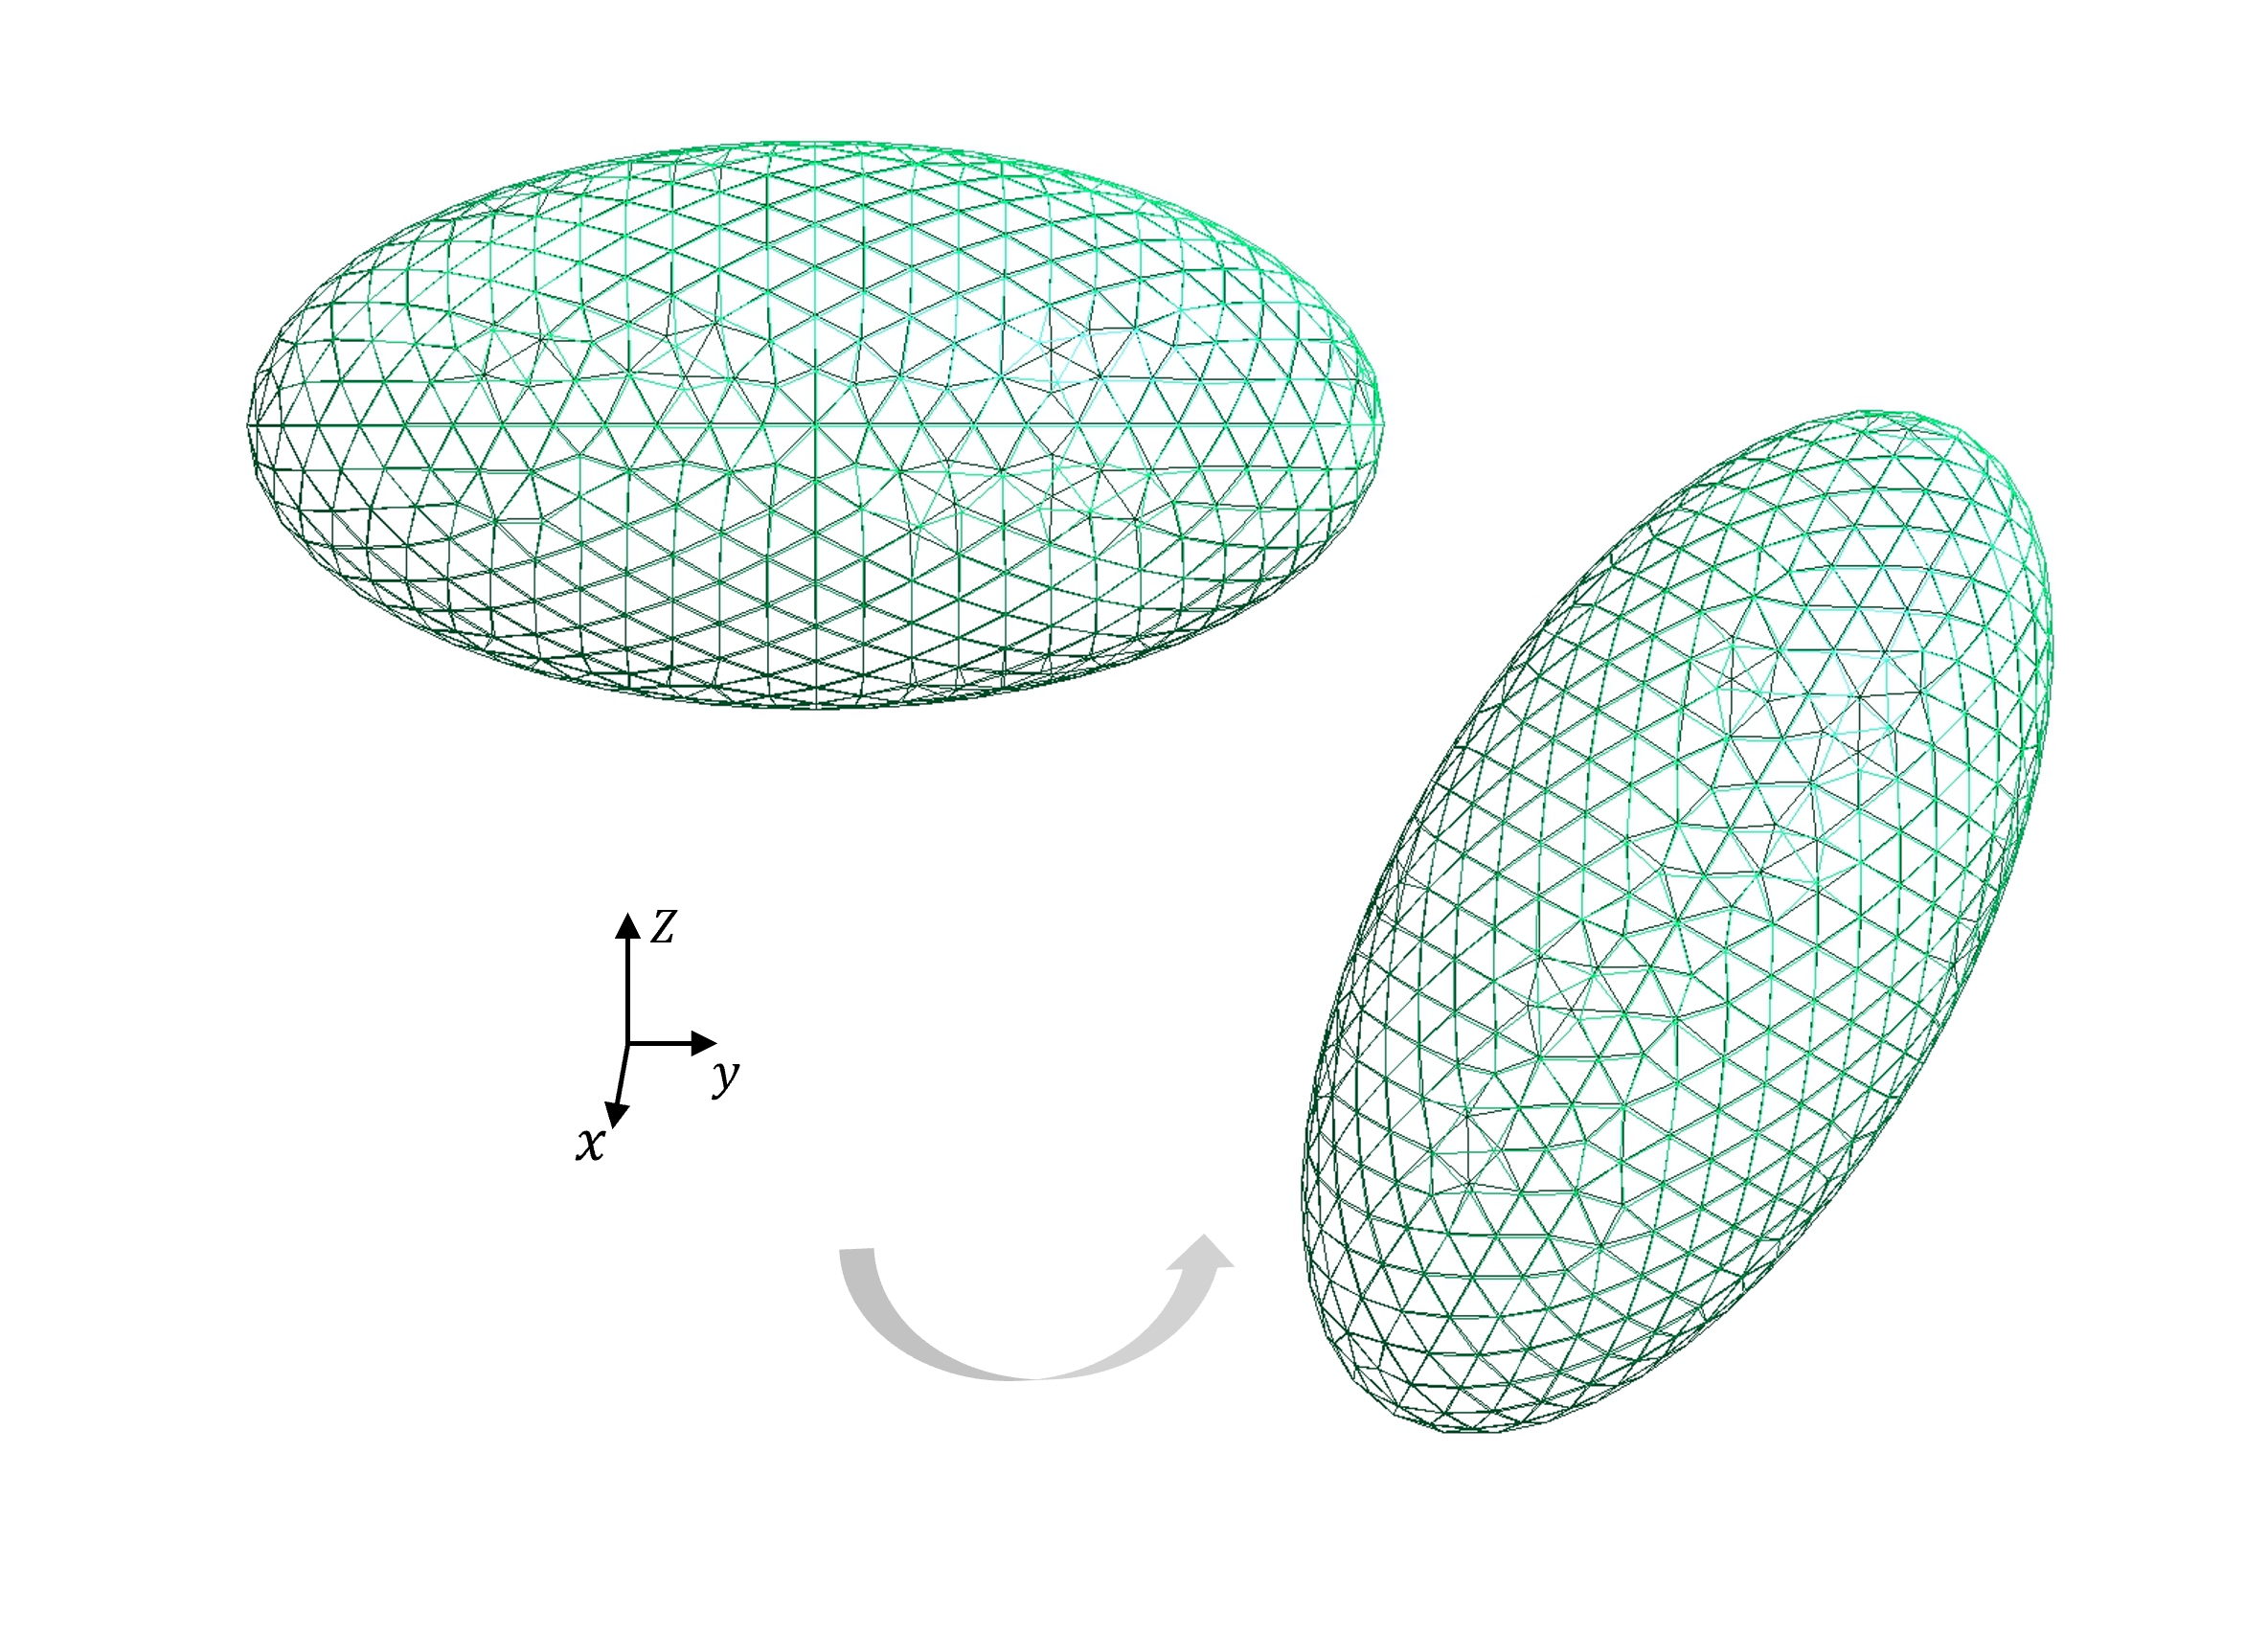
\includegraphics[scale = 0.07]{figures/Ellipsoid_x_axis}
    \caption{Rotation around x-axis}
    \label{Rotation around x-axis}
    \end{subfigure}
    \caption{Two ellipsoids with or without rotation: when $h_\text{fine}$ = 0.05, $\text{dim}(\mathsf{V}_{\mathrm{i}k}) = 5517$; 
    $h_\text{coarse}$ = 0.1, $\text{dim}(\mathsf{V}_{\mathrm{i}k}) = 1498$. The principal semi-axes of two ellipsoids are $r_{1} = 0.5$ and $r_{2} = 1.0$.}
    \label{Two ellipsoids}
    \end{figure}

    \begin{figure}[H]
        \begin{subfigure}{\linewidth}
            \centering
            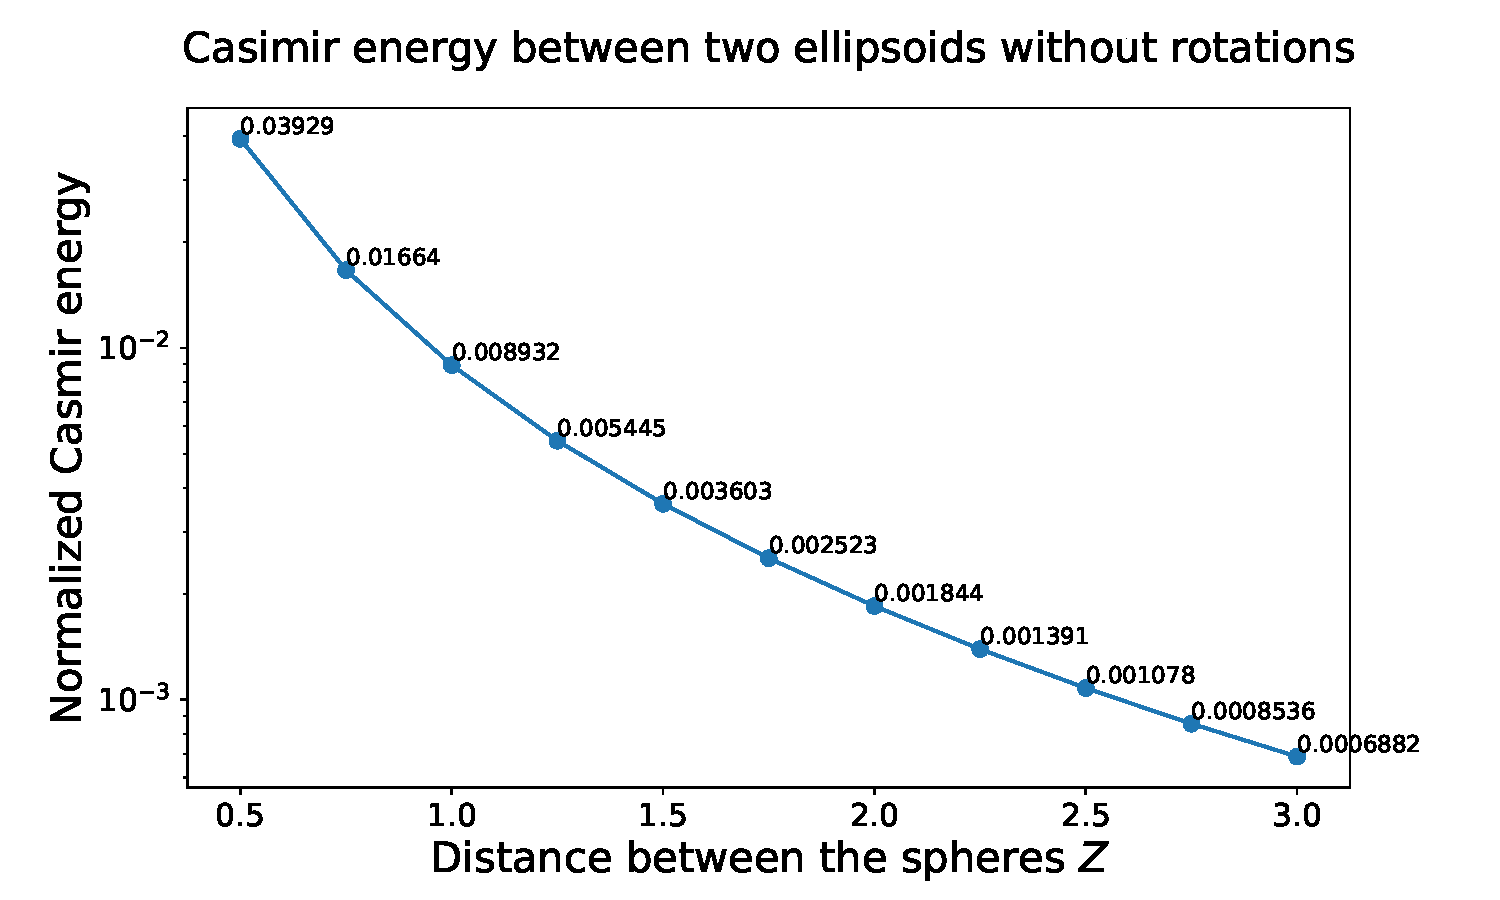
\includegraphics[scale = 0.5]{figures/CasE_ellipsoids.pdf}
            \caption{Casimir energy between two ellipsoids with different distances}
            \label{Casimir energy between two ellipsoids with different distances}
            \end{subfigure}\\[1ex]
    
        \begin{subfigure}{\linewidth}
        \centering
        \hspace*{-1cm}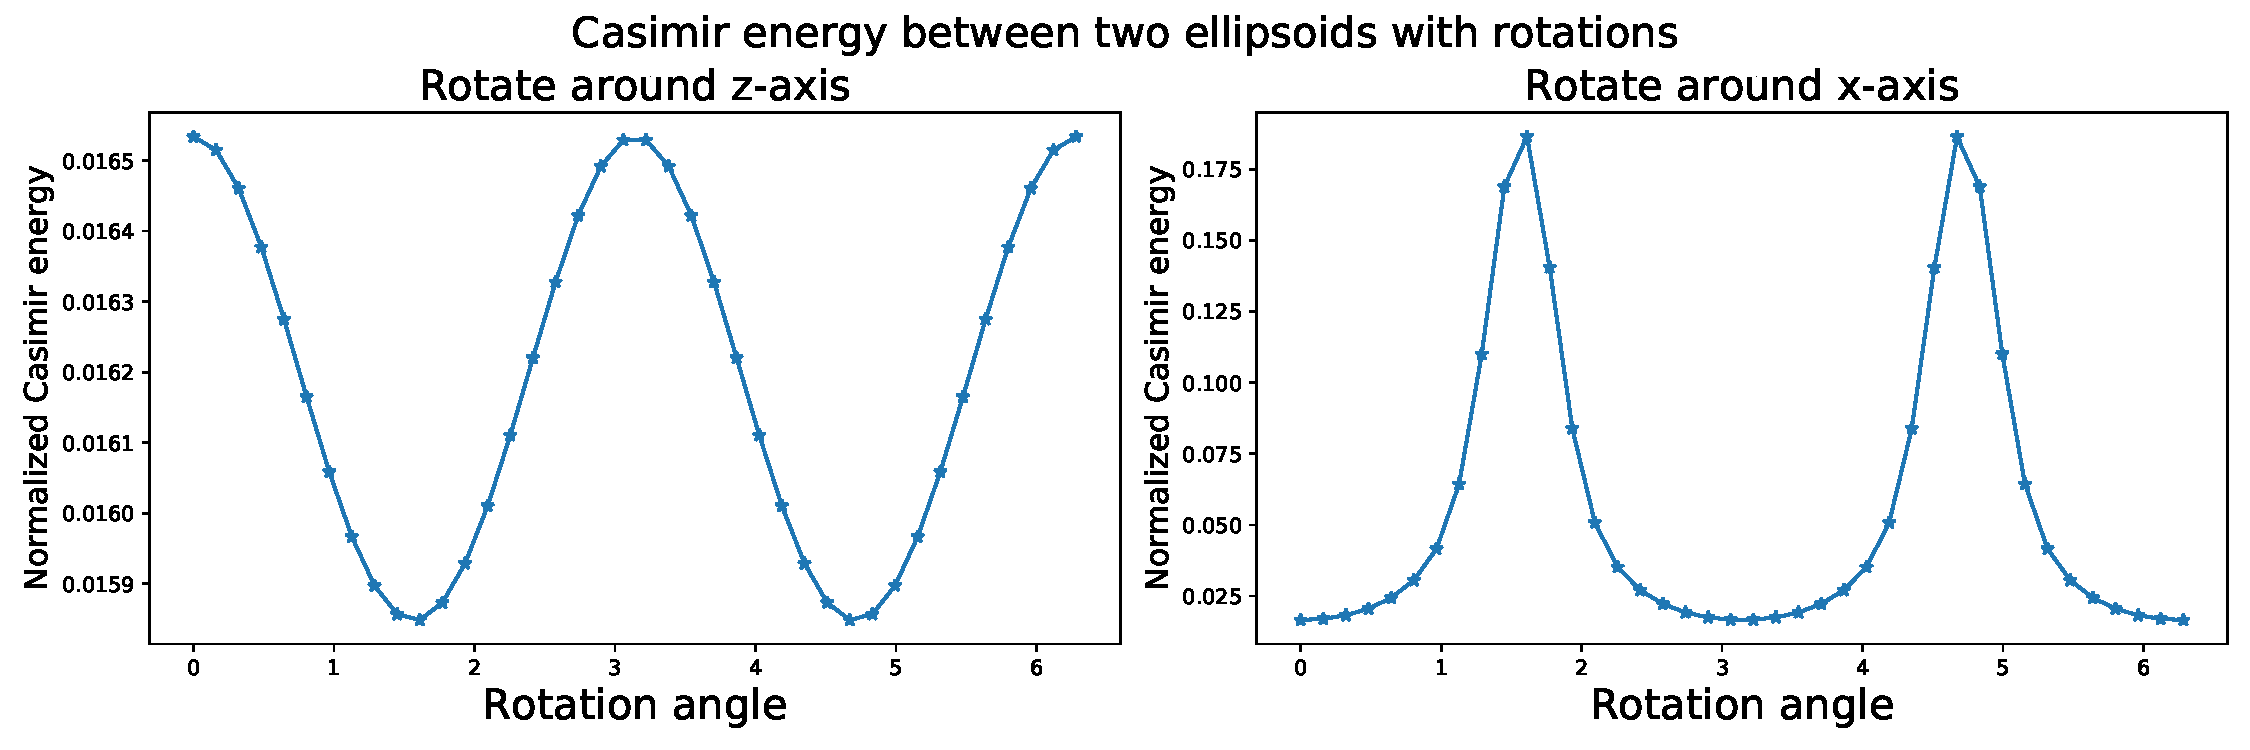
\includegraphics[scale = 0.45]{figures/CasE_ellipsoids_with_rotation.pdf}
        \caption{Casimir energy when one of the ellipsoids rotates}
        \label{Casimir energy when one of the ellipsoids rotates}
        \end{subfigure}
        \caption{The dependence of the Casimir energy and rotation angle of one of the ellipsoids.} 
        \end{figure}

Now, consider 4 ellipsoids located on the vertices of a regular tetrahedron with edge length $l = 2$ (Figure \ref{Four ellipsoids with or without rotations}) and 
the principal semi-axes of all these ellipsoids are $r_{1} = 0.6$ and $r_{2} = 0.3$. Figure \ref{Rotation inwards 4} and Figure \ref{Rotation outwards 4}
show the rotation of the ellipsoids inwards and outwards 360 degrees towards the centroid of this tetrahedron, separately. Afterwards, in order to use the Richardson extrapolation
method to estimate the Casimir energy, we evaluate the integral \eqref{KSSF and CasE} with the grid size set as $h_{\text{fine}} = 0.05$ and 
$h_{\text{coarse}} = 0.03$. Note that the number of the scatterers has increased to four, the matrices $\mathsf{V}_{\mathrm{i}k}$ and 
$\tilde{\mathsf{V}}_{\mathrm{i}k}$ have become to 4 by 4 block and diagonal block matrix, 
respectively. From the Figure \ref{Four ellipsoids}, it shows that the Casimir energy between these four ellipsoids changes periodically with the rotation.

\begin{figure}[H]
    \begin{subfigure}{\linewidth}
        \centering
        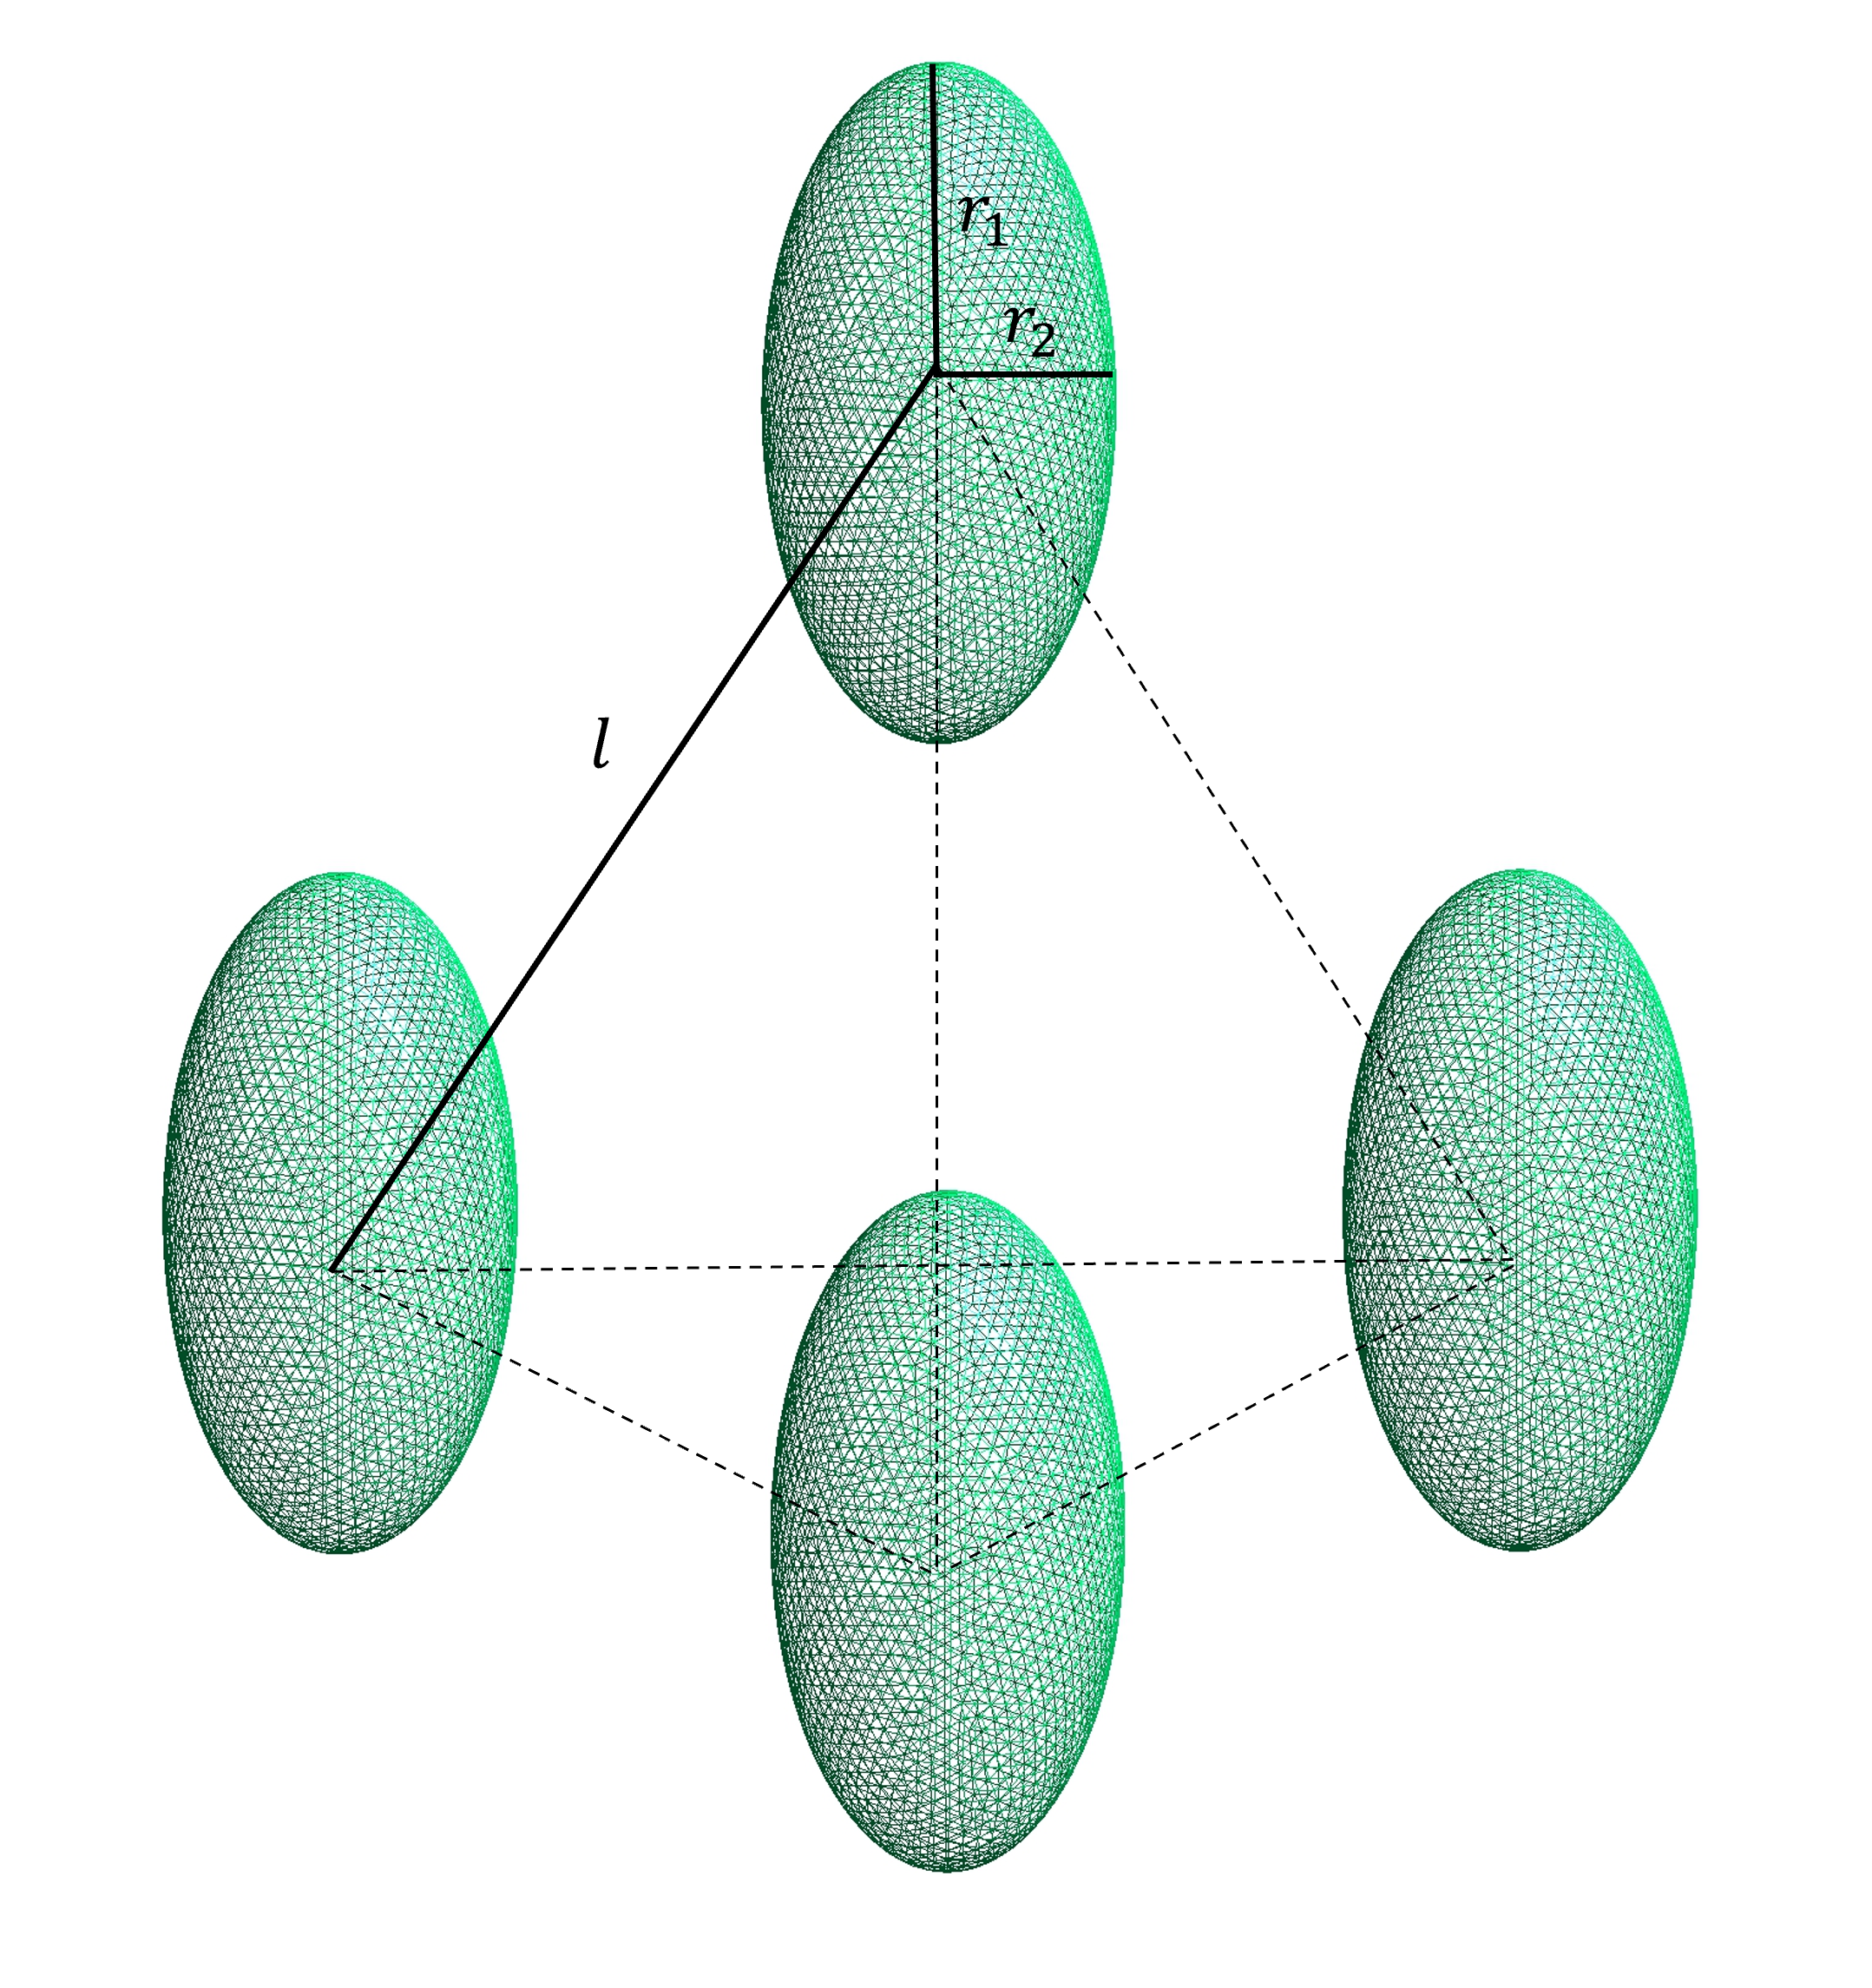
\includegraphics[scale = 0.4]{figures/4_ellip}
        \caption{No rotation}
        \label{No rotation 4}
        \end{subfigure}\\[1ex]
    \begin{subfigure}{.5\linewidth}
    \centering
    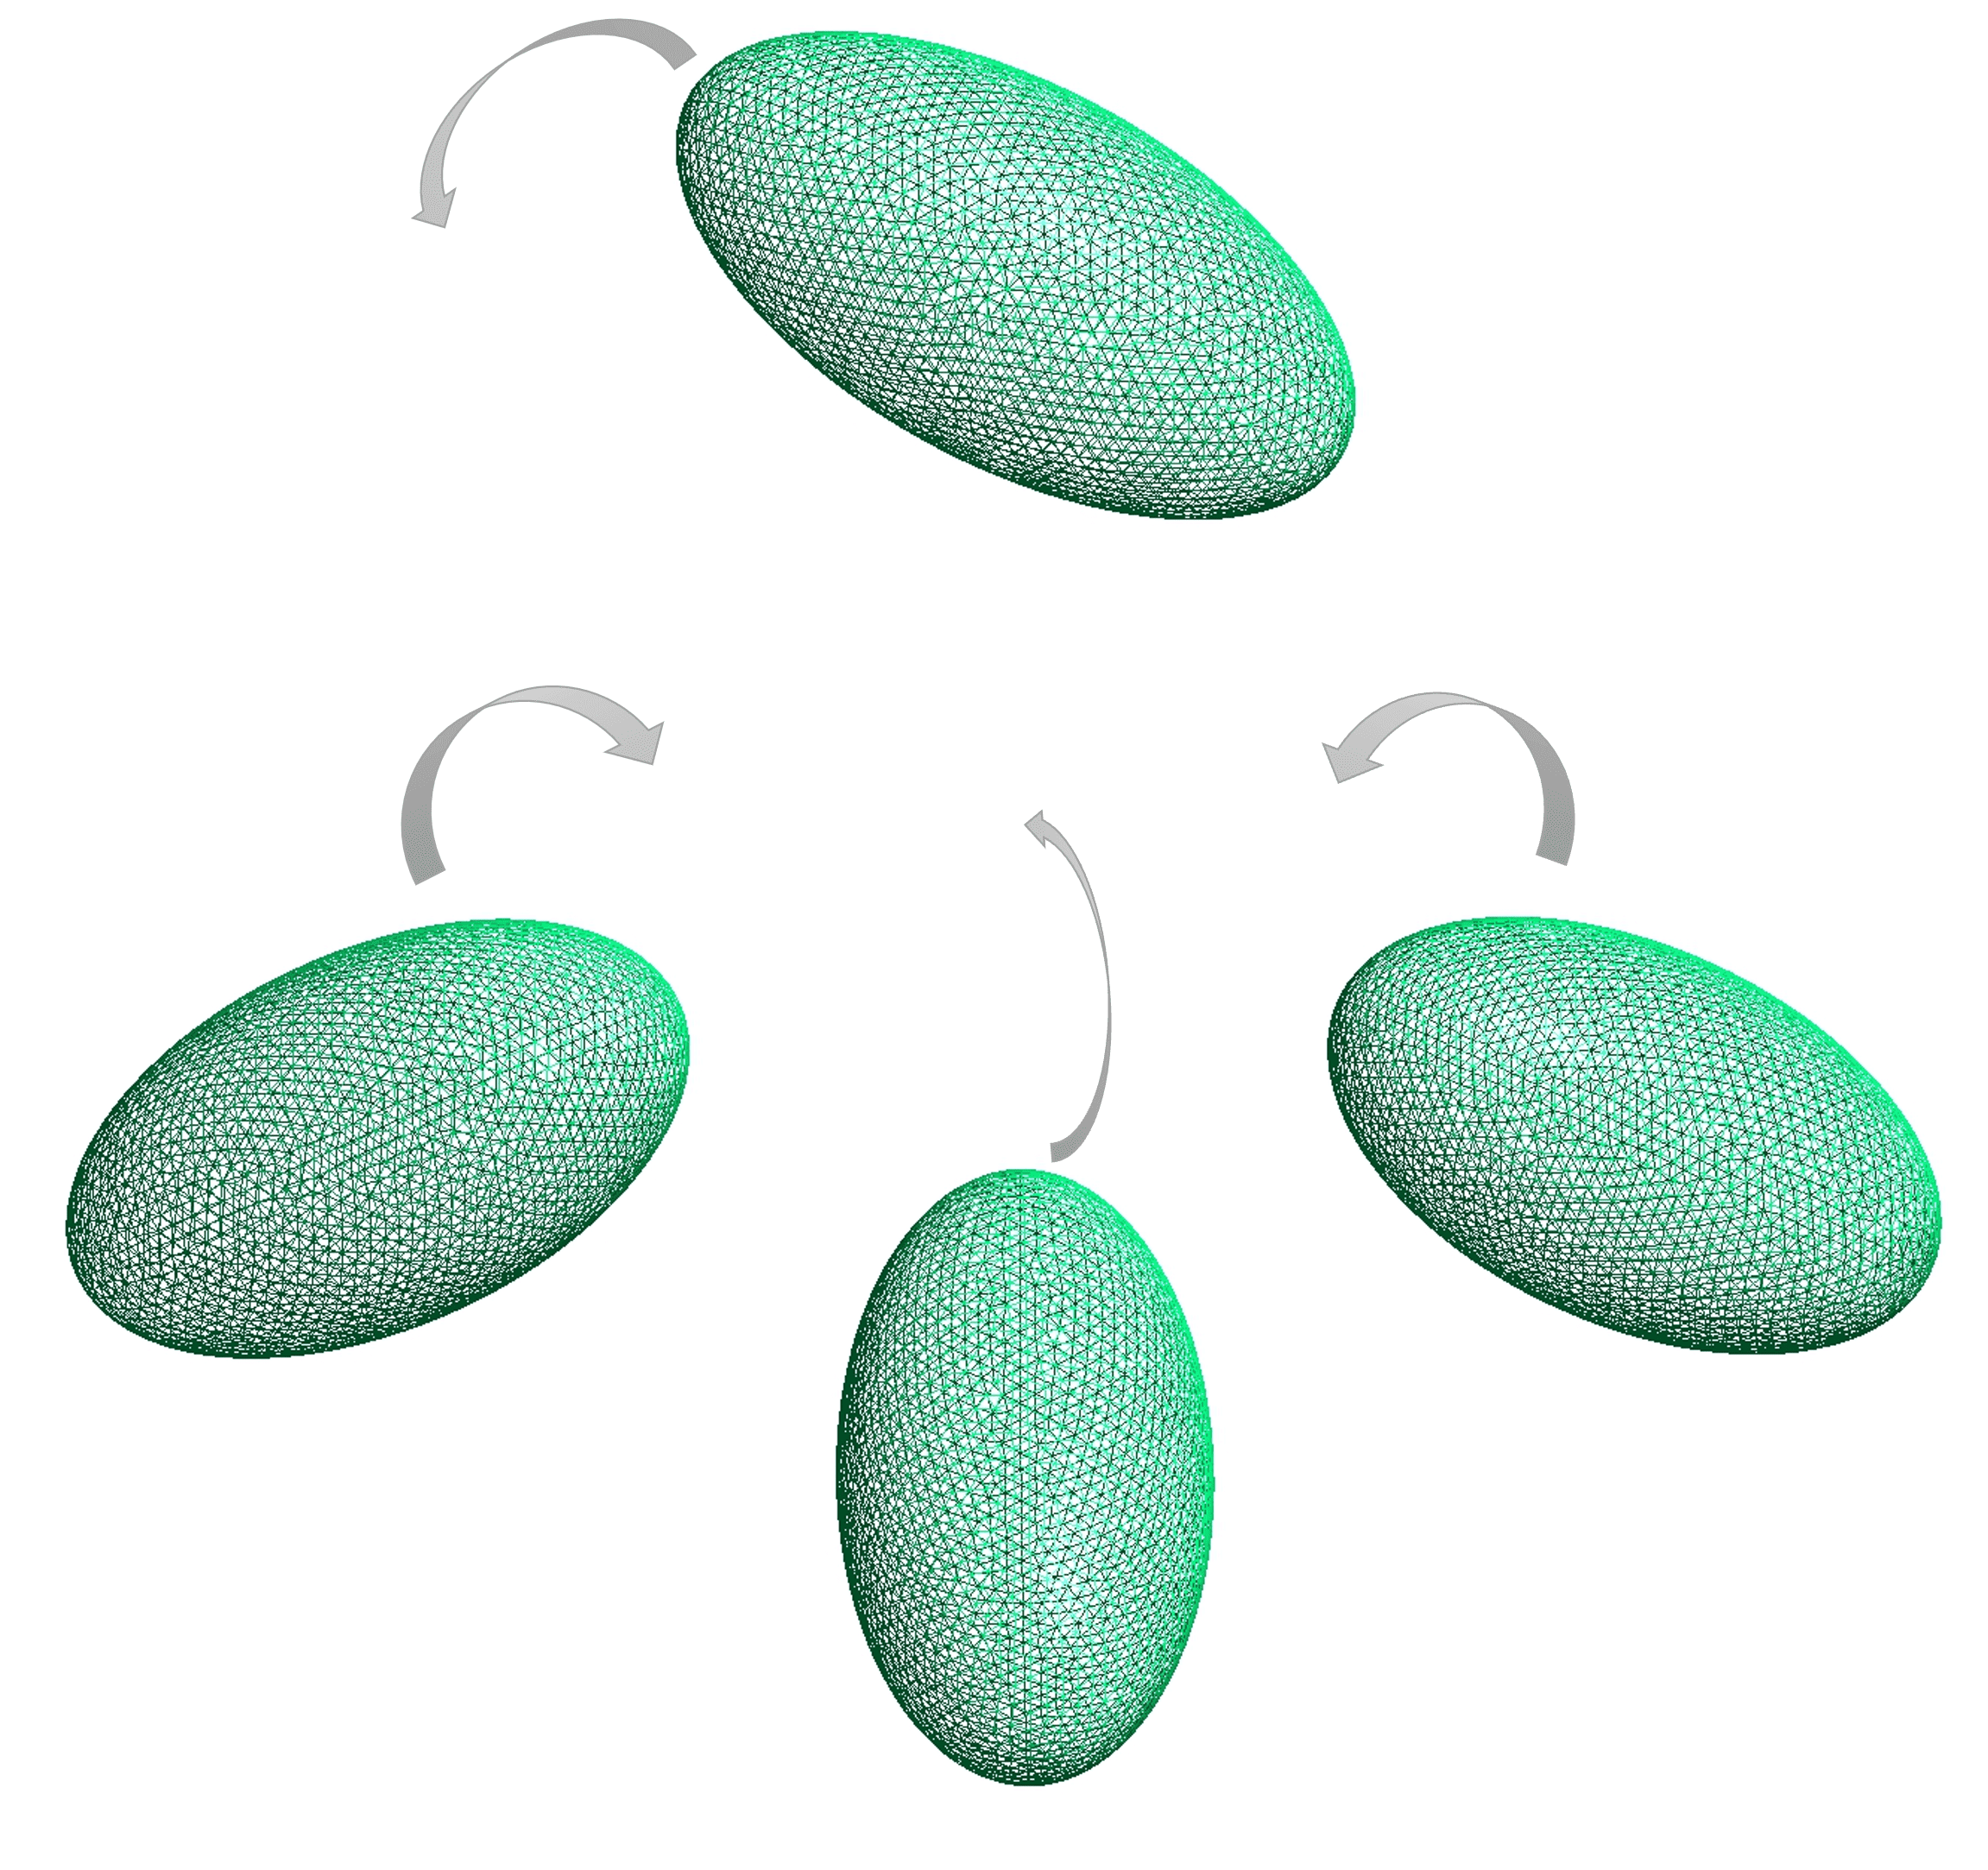
\includegraphics[scale = 0.09]{figures/4_ellip_in}
    \caption{Rotation inwards}
    \label{Rotation inwards 4}
    \end{subfigure}%
    \begin{subfigure}{.5\linewidth}
    \centering
    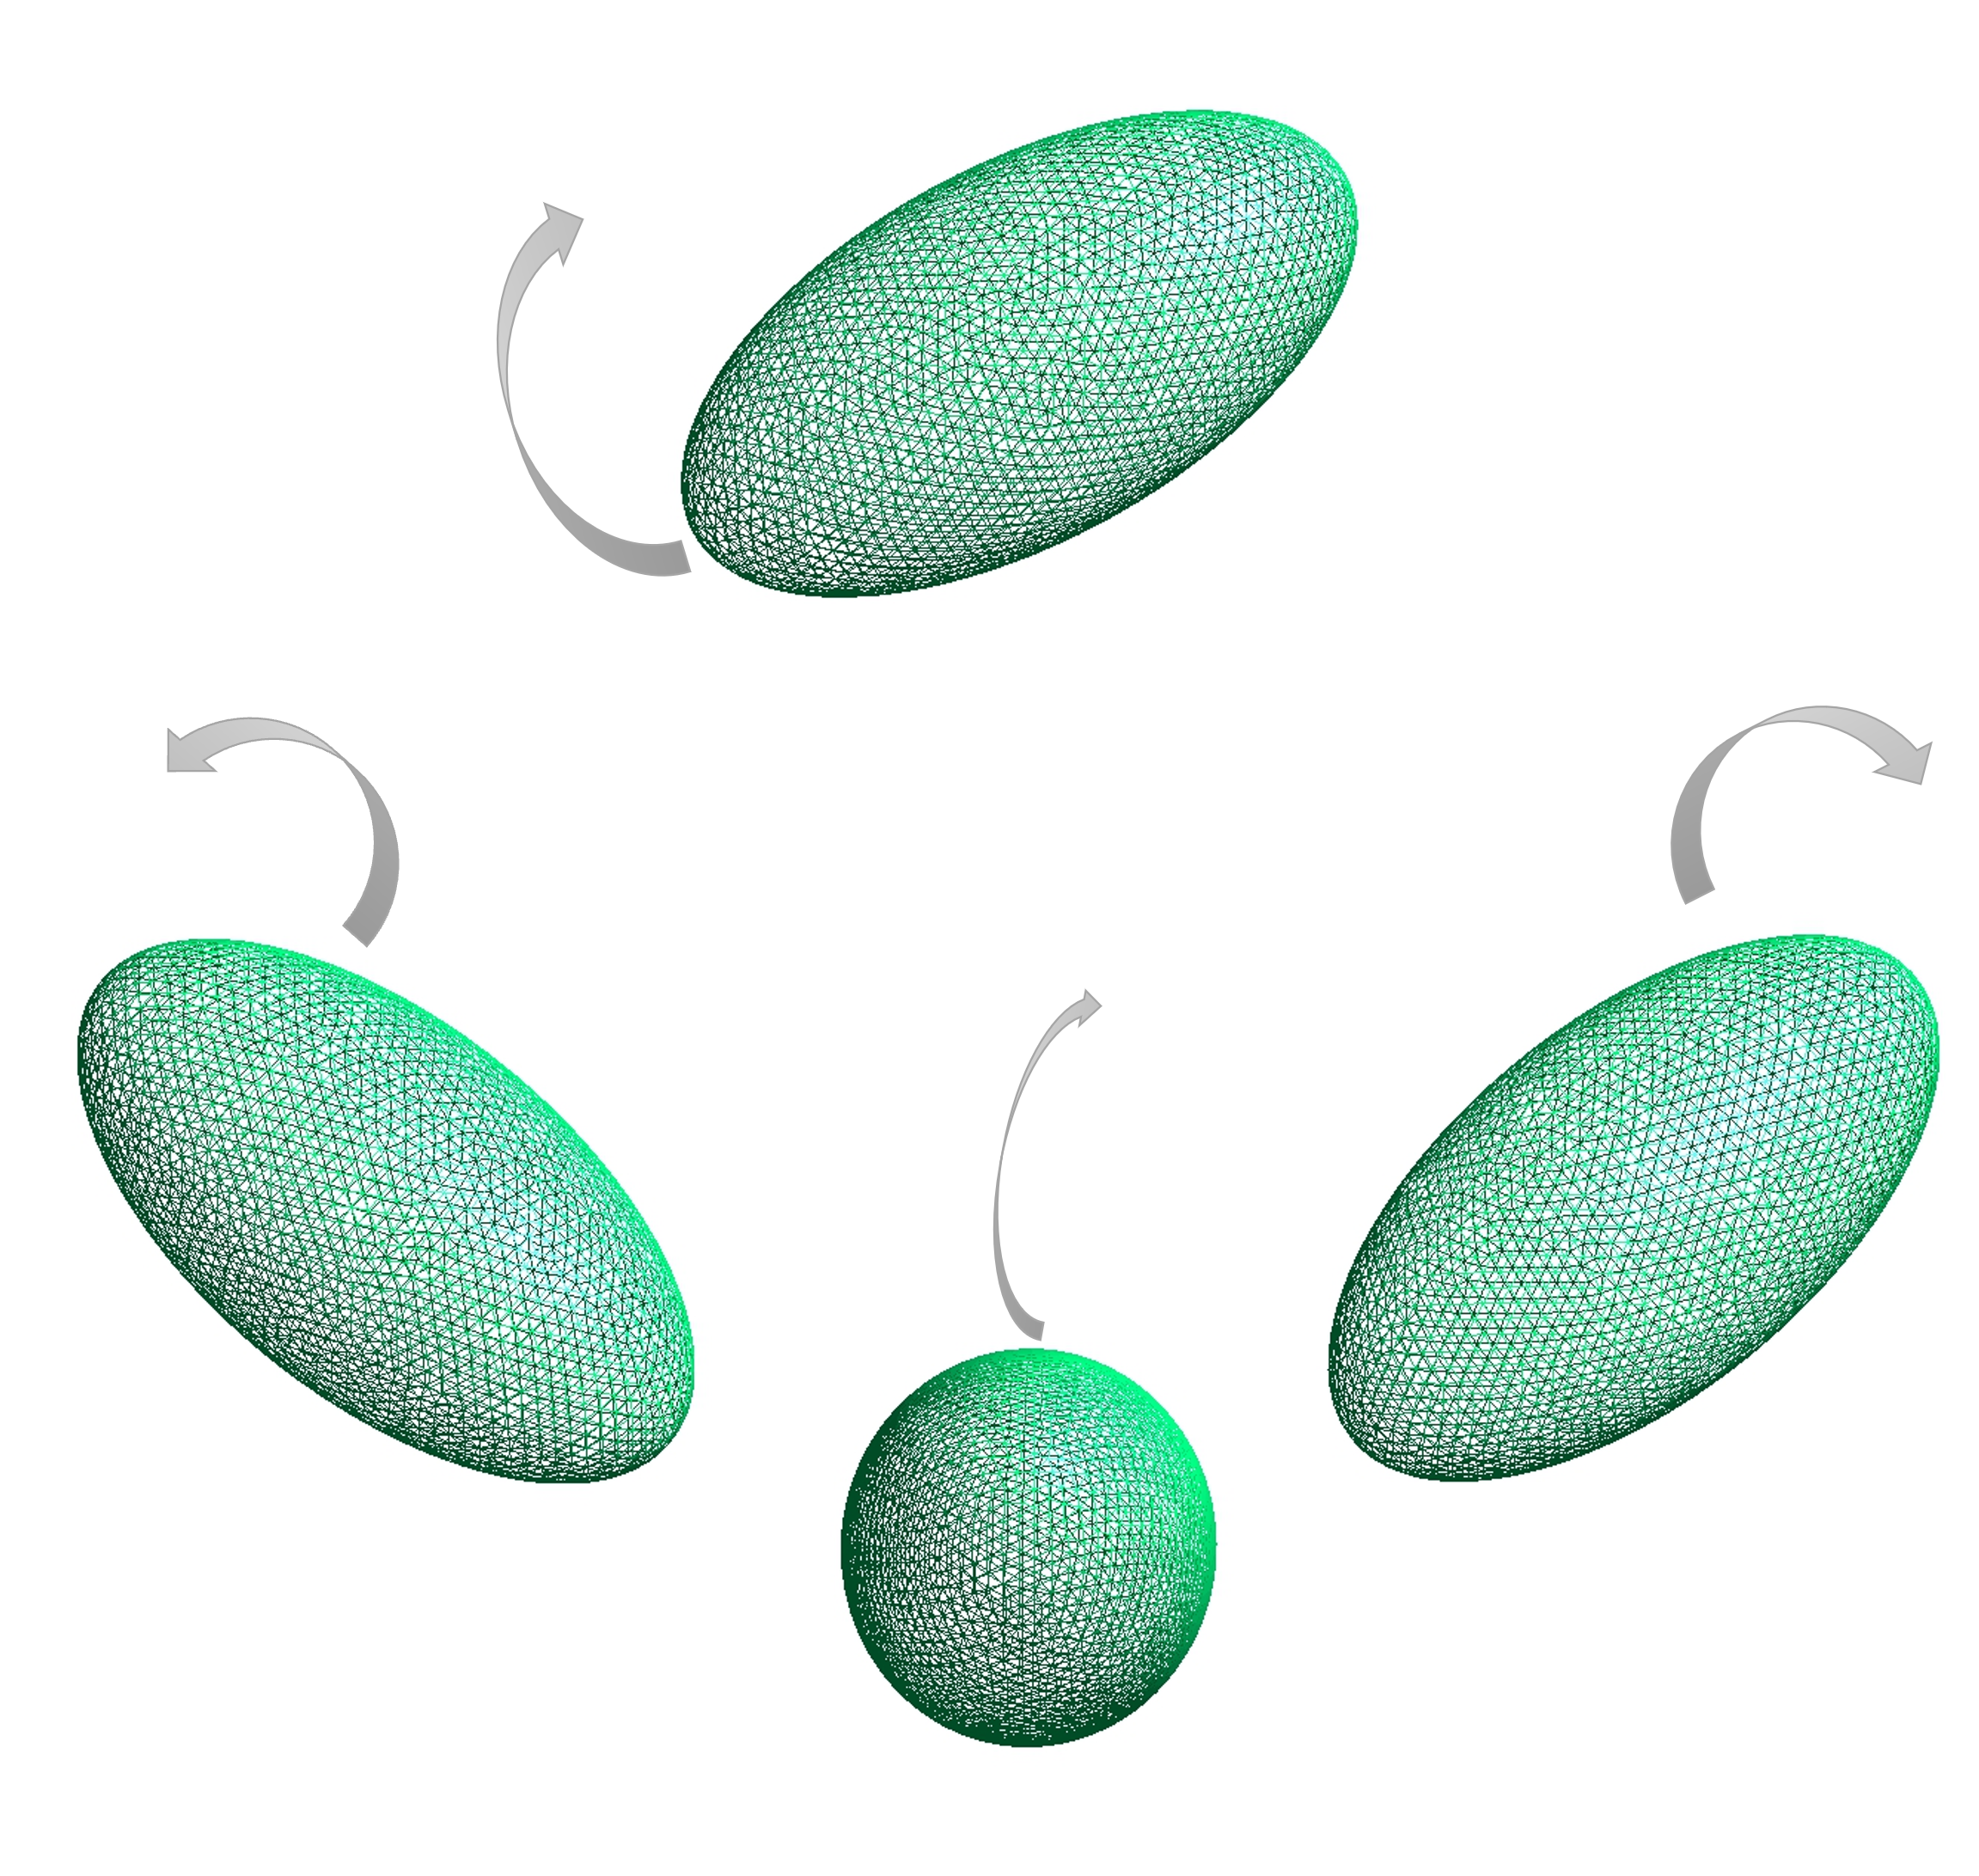
\includegraphics[scale = 0.4]{figures/4_ellip_out}
    \caption{Rotation outwards}
    \label{Rotation outwards 4}
    \end{subfigure}
    \caption{Four ellipsoids with or without rotations:  when $h_\text{fine}$ = 0.03, $\text{dim}(\mathsf{V}_{\mathrm{i}k}) = 11024$; 
    $h_\text{coarse}$ = 0.05, $\text{dim}(\mathsf{V}_{\mathrm{i}k}) = 4160$. The principal semi-axes of these ellipsoids are $r_{1} = 0.6$ and $r_{2} = 0.3$
    and they locate on the vertices of a regular octahedron with edge length $l = 2$.}
    \label{Four ellipsoids with or without rotations}
    \end{figure}

    \begin{figure}[H]
        \centering
        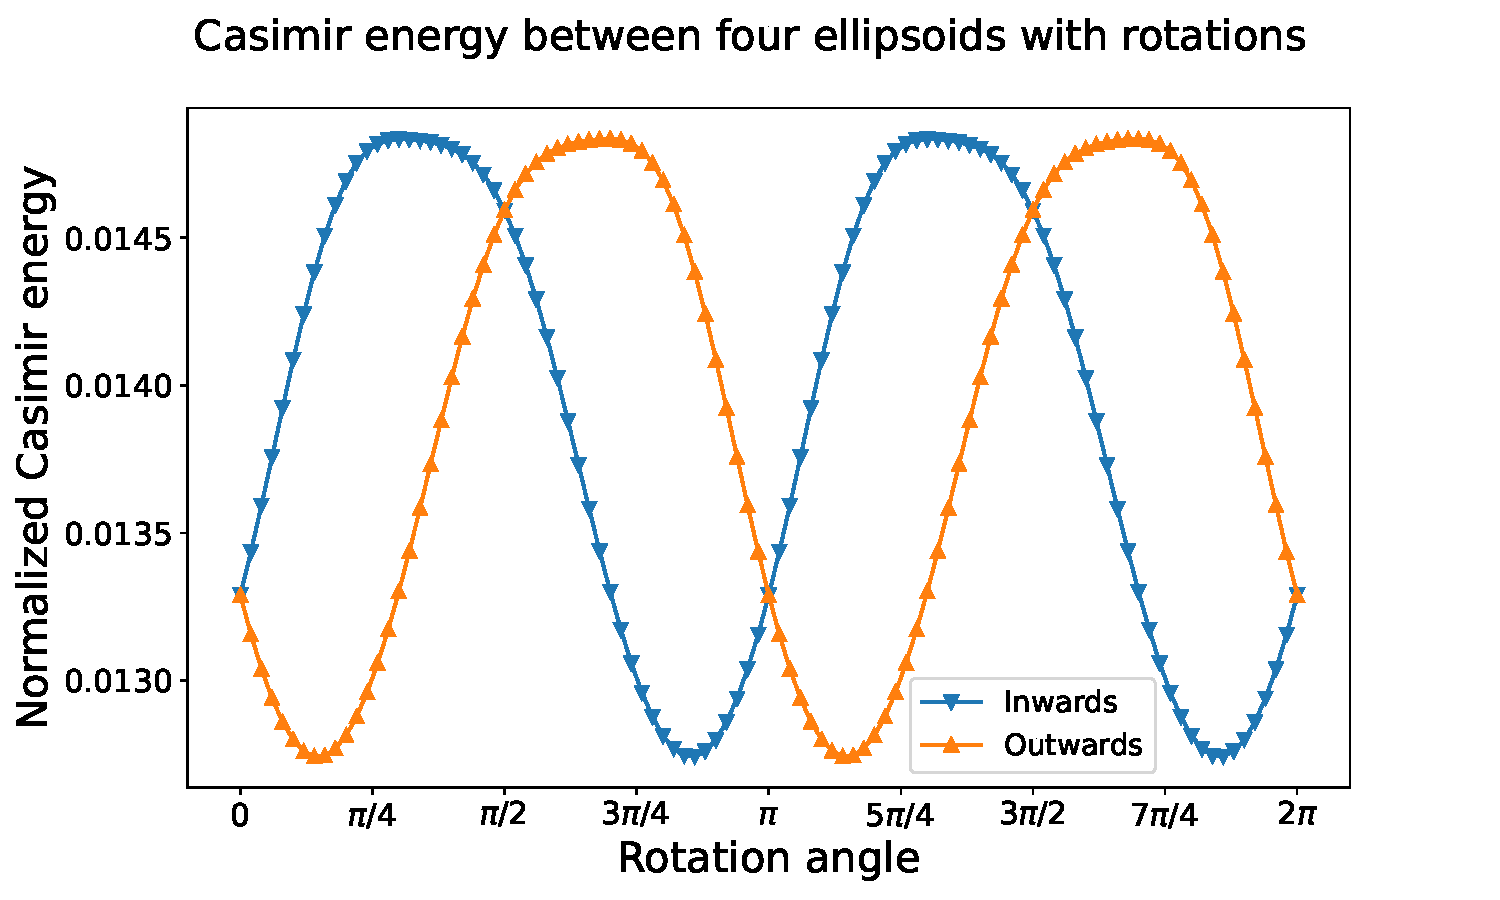
\includegraphics[scale = 0.5]{figures/CasE_4_ellip.pdf}
        \caption{The dependence of the Casimir energy and rotation angle of one of the ellipsoids. Inwards towards the centroid case (solid blue square).
        Outwards towards the centroid case (solid orange triangle).}
        \label{Four ellipsoids}
    \end{figure}

  The scatterers of the last example are described inside the Figure \ref{Six ellipsoids with or without rotations}. These six ellipsoids locate on the 
  vertices of a regular octahedron with edge length $l = 2$ and again the principal semi-axes of all these ellipsoids are $r_{1} = 0.6$ and $r_{2} = 0.3$ (shown 
  in the Figure \ref{Six ellipsoids with or without rotations}). This time, the ellipsoids rotate inwards and outwards 360 degrees towards the centroid of 
  this octahedron (Figure \ref{Rotation inwards 6} and Figure \ref{Rotation outwards 6}). By closely looking at these two rotation figures, we can notice that 
  Figure \ref{Rotation inwards 6} can be obtained by rotating Figure \ref{Rotation outwards 6} 180 degrees. Therefore, the Casimir energies for the inwards and 
  outwards cases are the same. Figure \eqref{Six ellipsoids} shows how the Casimir energy changes among these six ellipsoids as they rotate. 

\begin{figure}[H]
    \begin{subfigure}{\linewidth}
        \centering
        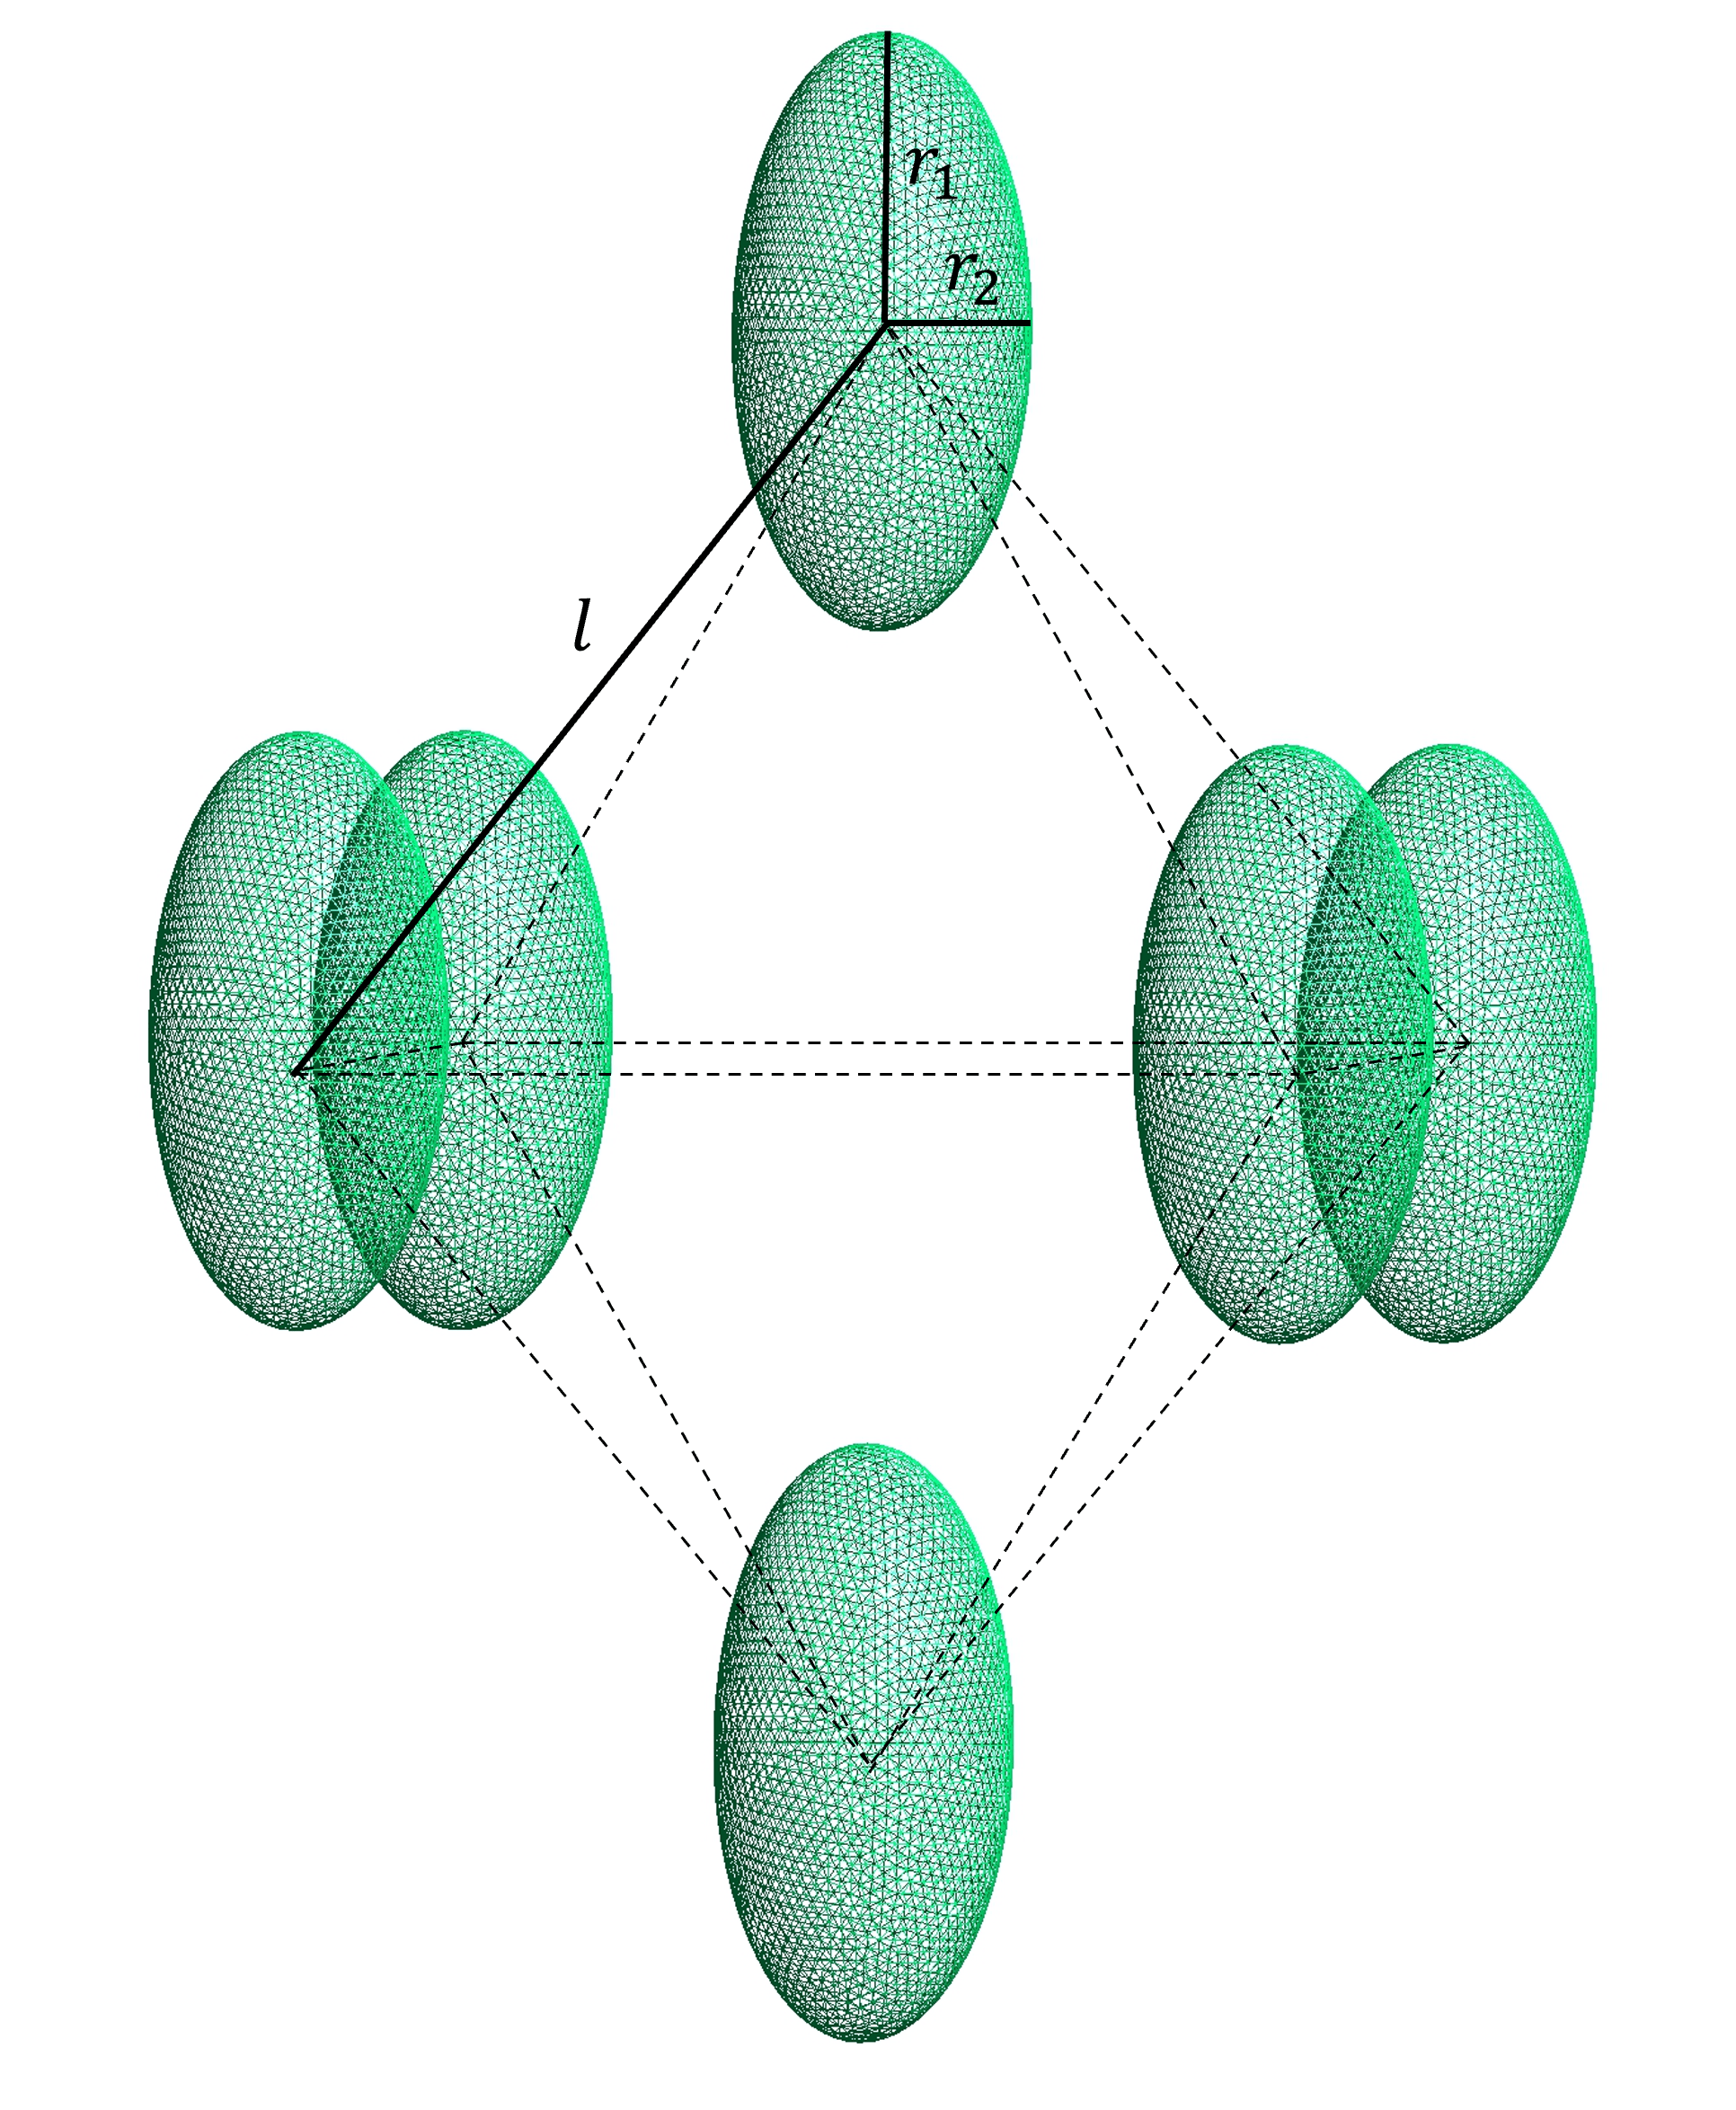
\includegraphics[scale = 0.4]{figures/6_ellip}
        \caption{No rotation}
        \label{No rotation 6}
        \end{subfigure}\\[1ex]
    \begin{subfigure}{.5\linewidth}
    \centering
    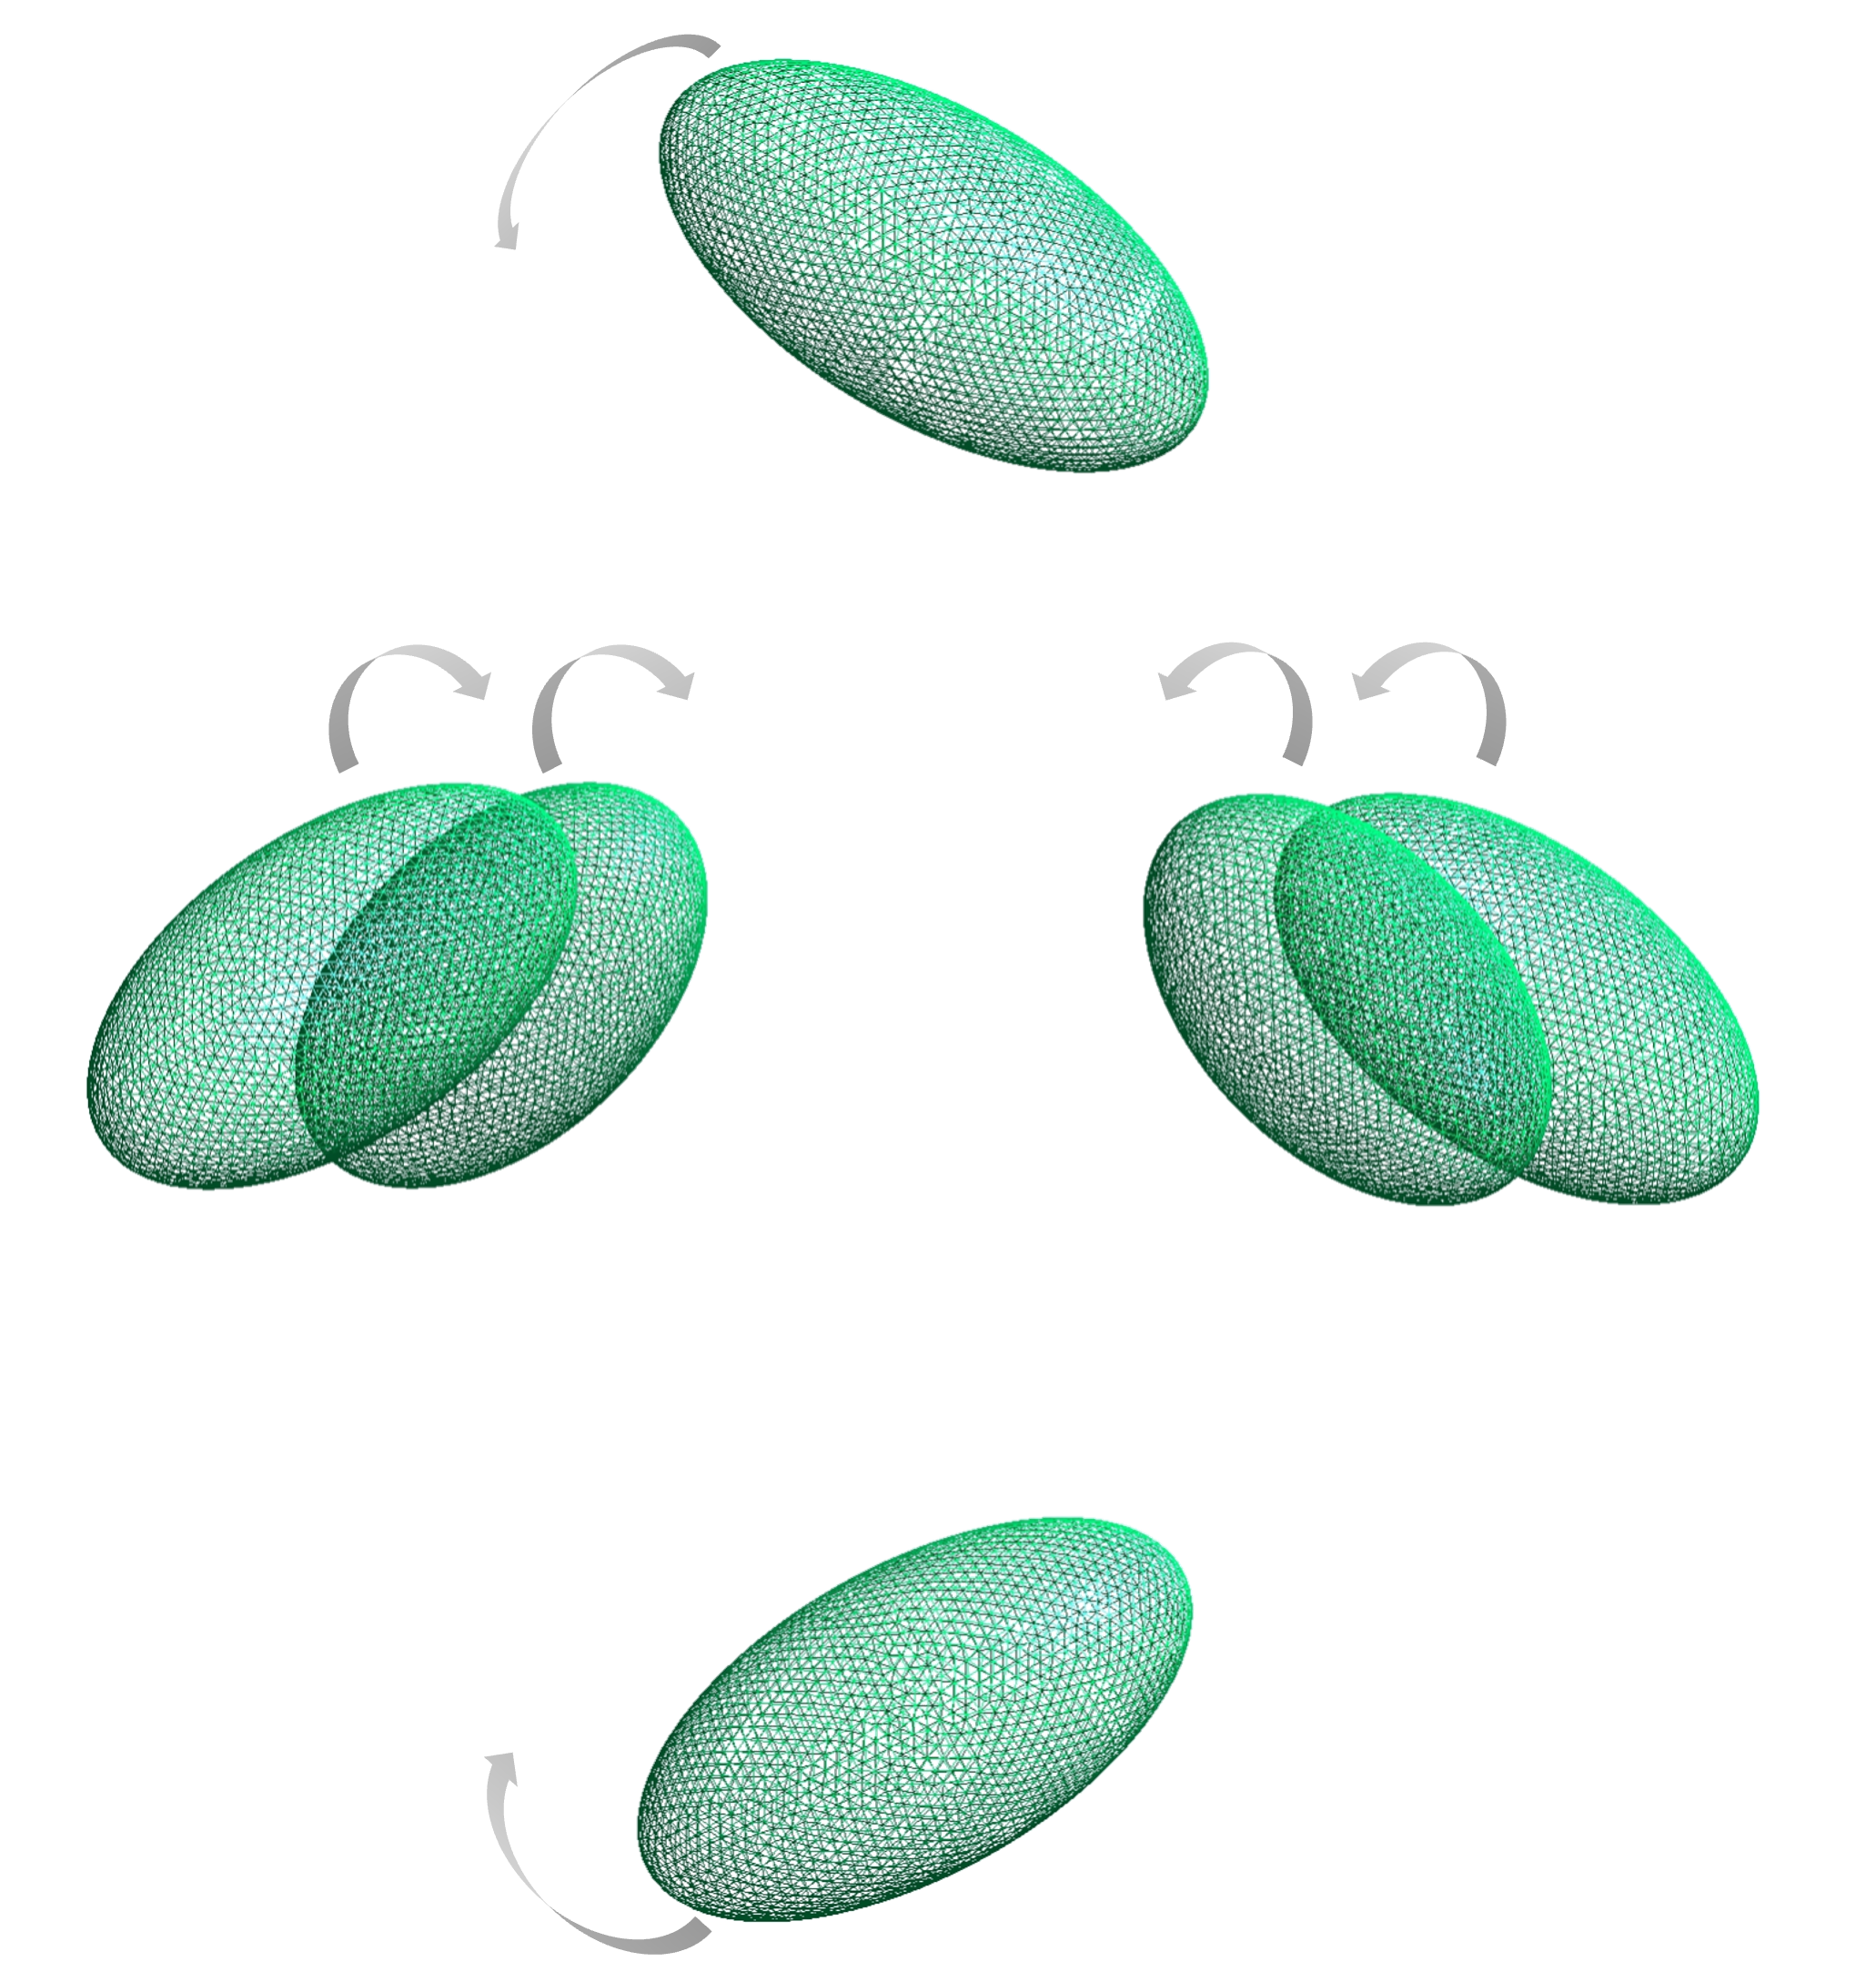
\includegraphics[scale = 0.4]{figures/6_ellip_in}
    \caption{Rotation inwards}
    \label{Rotation inwards 6}
    \end{subfigure}%
    \begin{subfigure}{.5\linewidth}
    \centering
    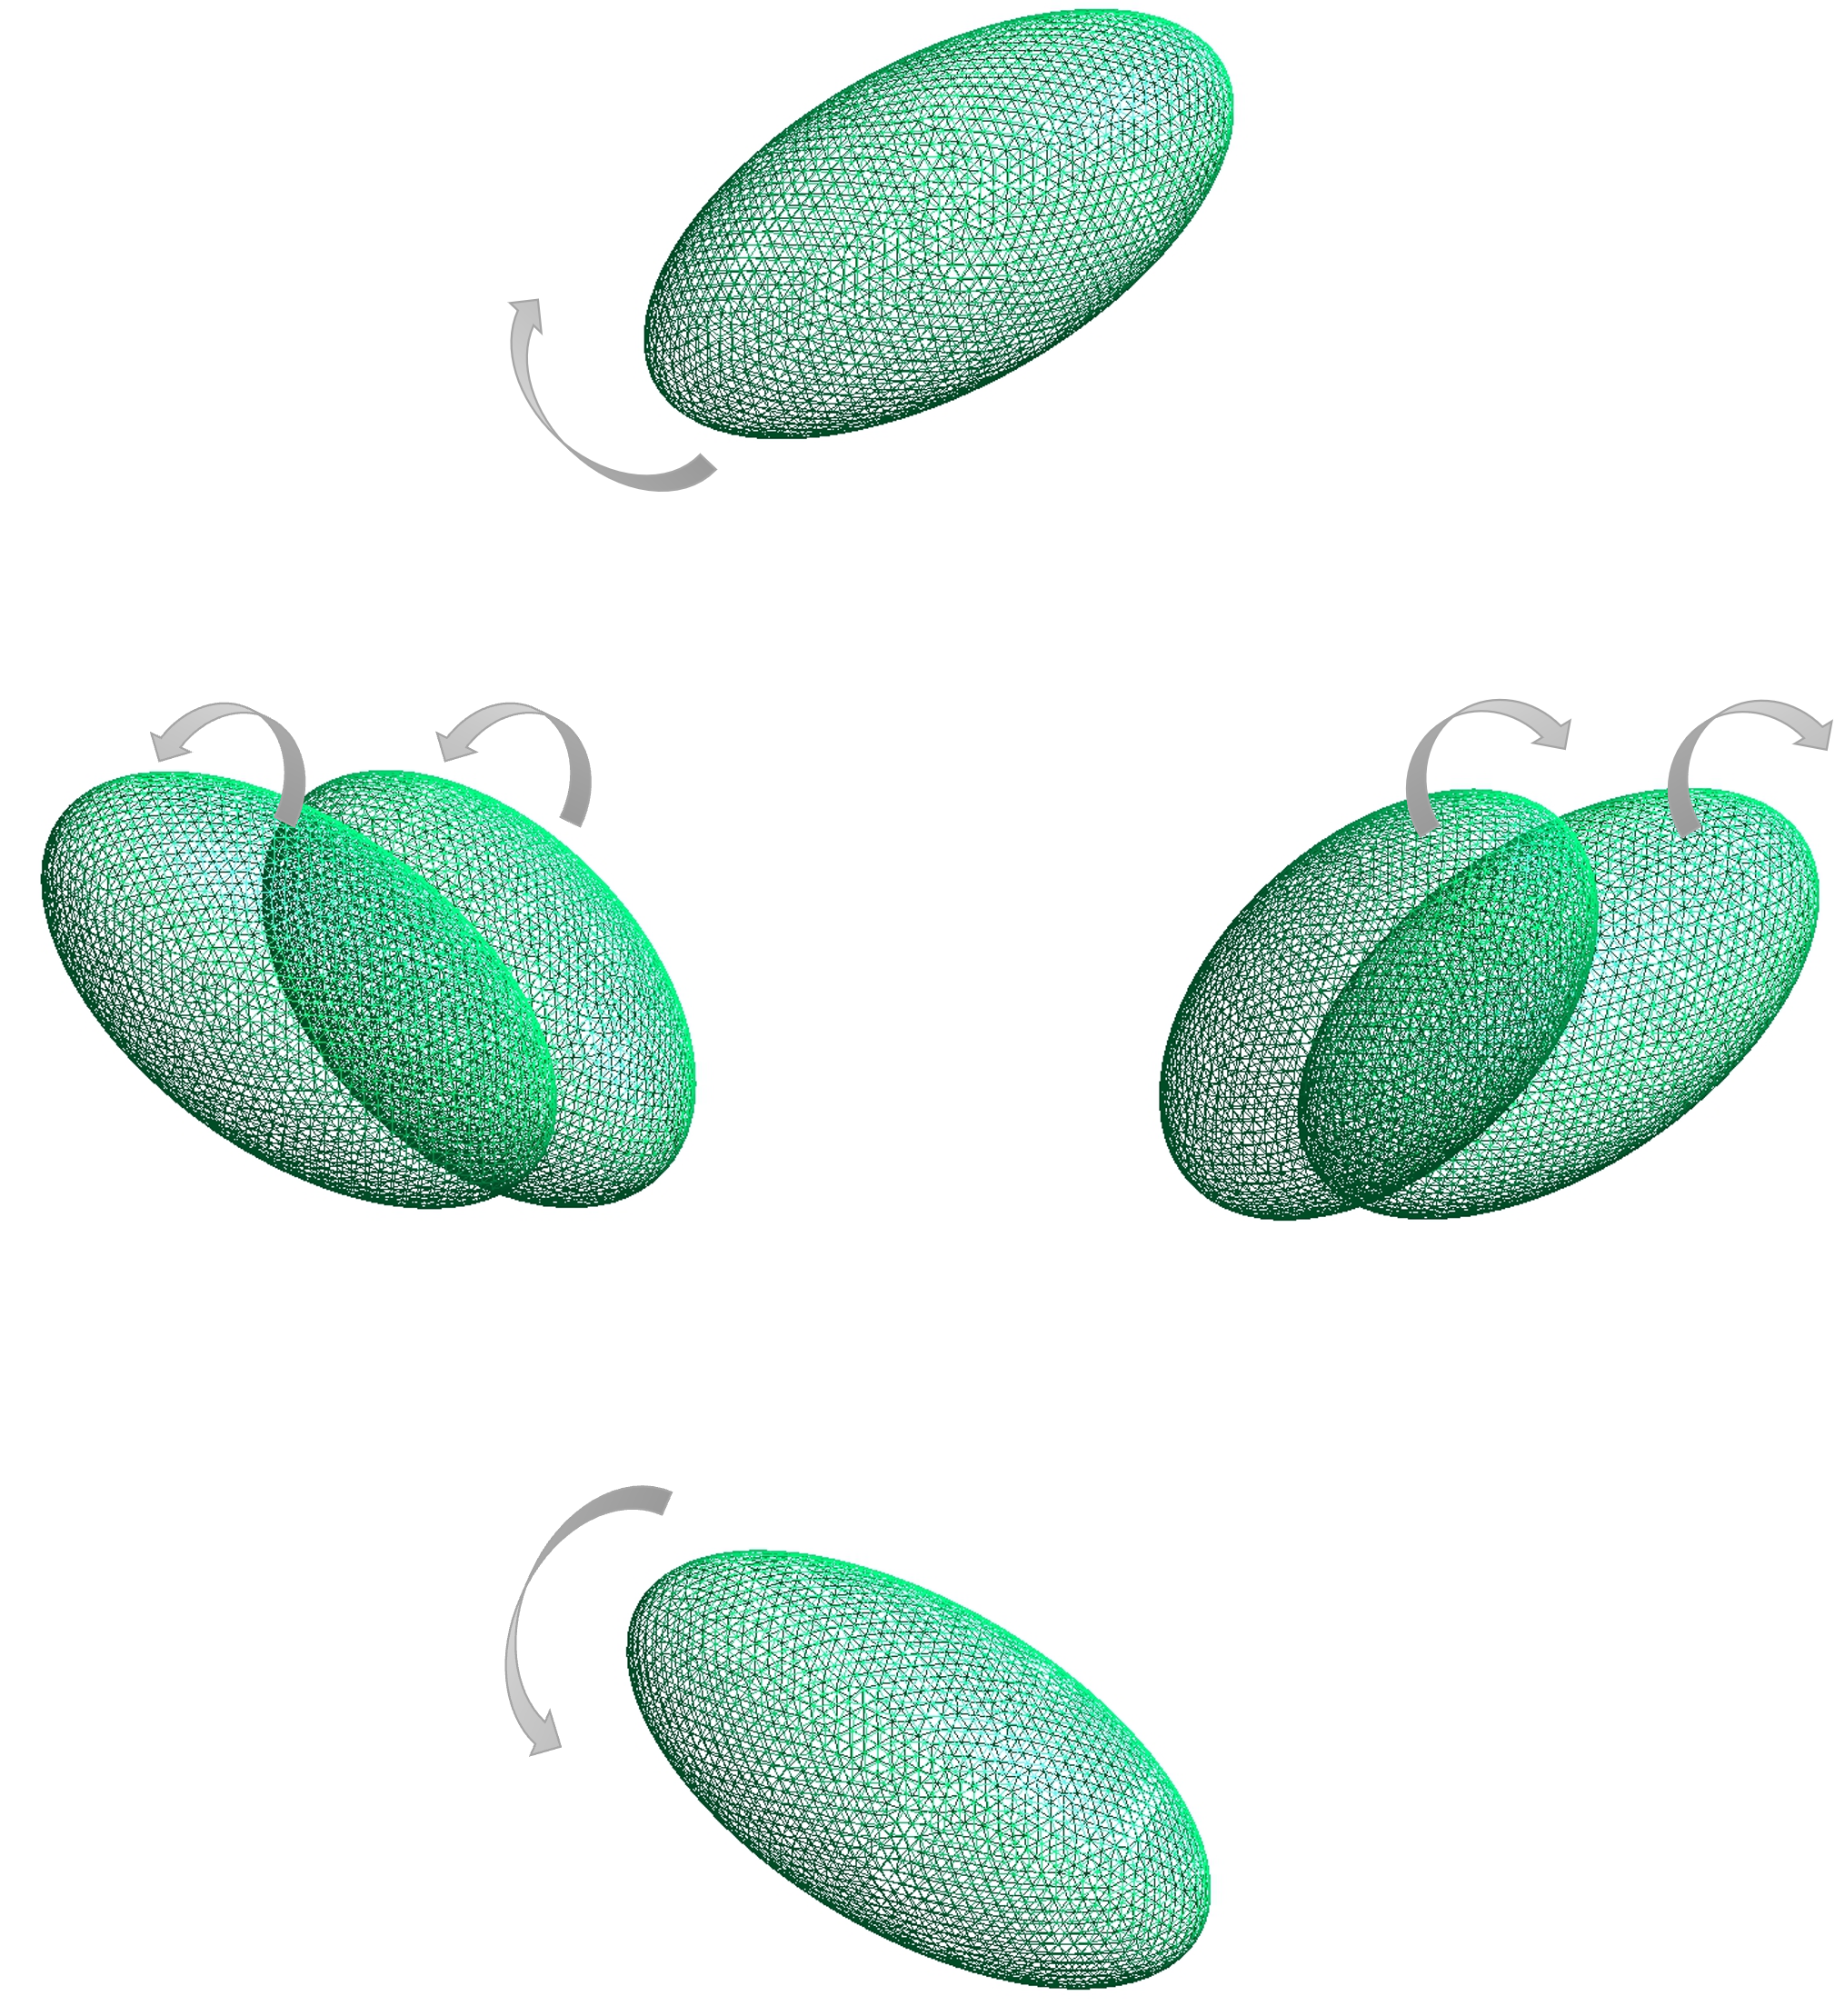
\includegraphics[scale = 0.4]{figures/6_ellip_out}
    \caption{Rotation outwards}
    \label{Rotation outwards 6}
    \end{subfigure}
    \caption{Six ellipsoids with or without rotations: when $h_\text{fine}$ = 0.03, $\text{dim}(\mathsf{V}_{\mathrm{i}k}) = 16536$;  $h_\text{coarse}$ = 0.05, $\text{dim}(\mathsf{V}_{\mathrm{i}k}) = 6240$.
    The principal semi-axes of these ellipsoids are $r_{1} = 0.6$ and $r_{2} = 0.3$
    and they locate on the vertices of a regular octahedron with edge length $l = 2$.}
    \label{Six ellipsoids with or without rotations}
    \end{figure}

    \begin{figure}[H]
        \centering
        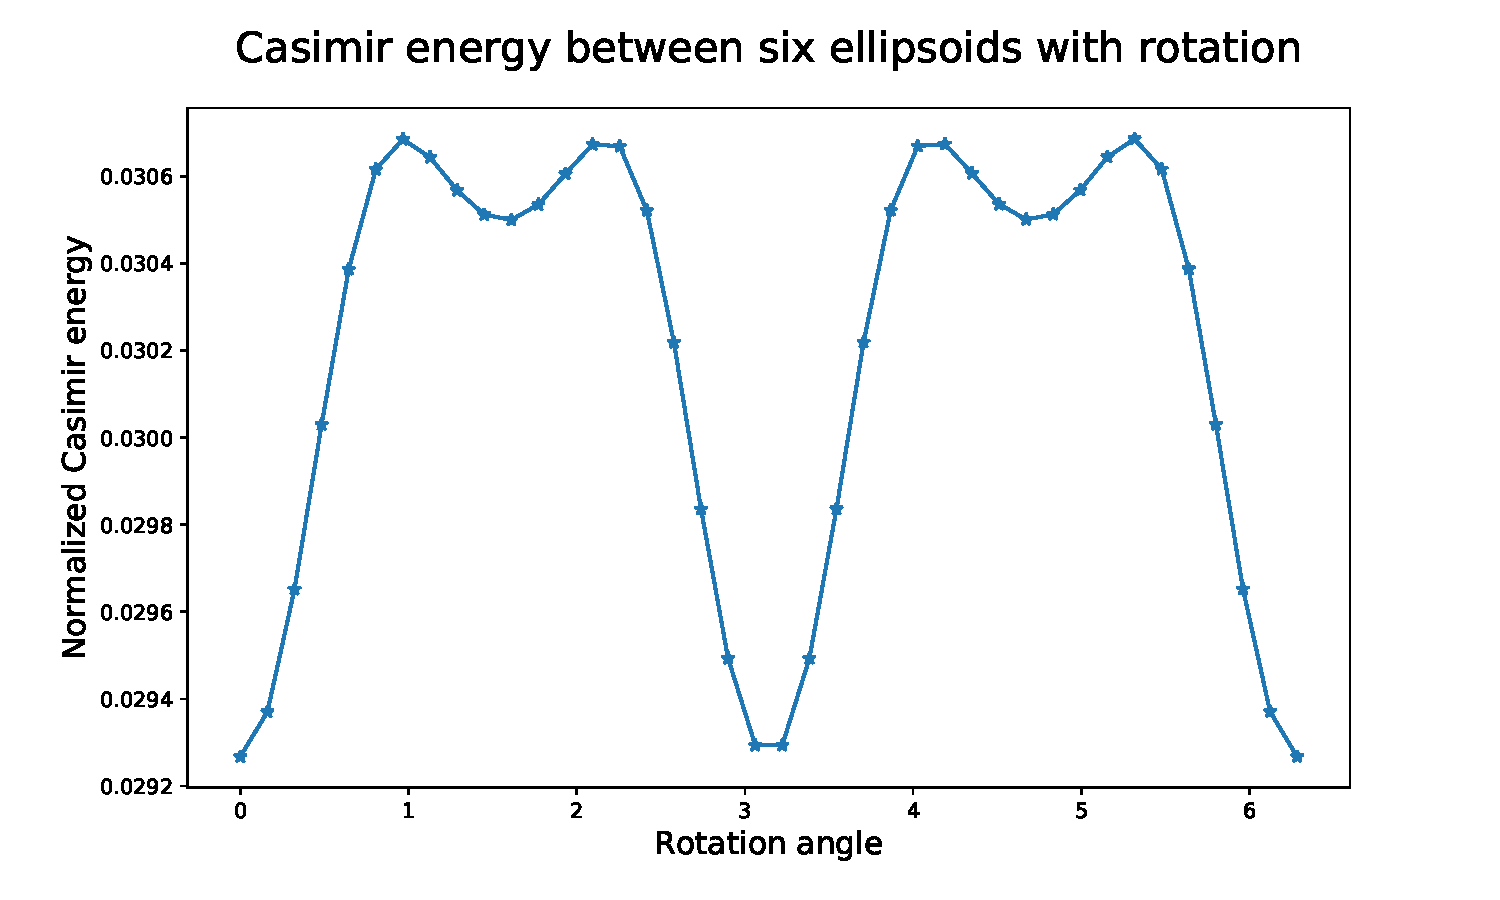
\includegraphics[scale = 0.5]{figures/CasE_6_ellip.pdf}
        \caption{The dependence of the Casimir energy and rotation angle of one of the ellipsoids.}
        \label{Six ellipsoids}
    \end{figure}